%-----------------------------------------------------------------------------%
% Set metadata for use with pdfx
%\begingroup\newif\ifmy
%\IfFileExists{\jobname.xmpdata}{}{\mytrue}
%\ifmy
%\begin{filecontents*}{\jobname.xmpdata}
%\Title{Data Science Notes}
%\Author{Matthew Epland, Ph.D.}
%\Keywords{Data Science\sep Machine Learning\sep Statistics}
%\Copyright{CC-BY-4.0}
%\end{filecontents*}
%\fi\endgroup

% \Subject{TODO}

%-----------------------------------------------------------------------------%
% Set documentclass
\documentclass[nogradschool,singlespace,nobind]{dukedissertation_modified}

%-----------------------------------------------------------------------------%
% usepackages
\usepackage{amsmath,amssymb,bbm,bm} % https://ctan.org/pkg/bm
\usepackage{mathtools}
\usepackage{cancel}
\usepackage{graphicx}
\usepackage{xcolor}
\usepackage{textcomp} % needed to fix \mico \textmu from siunitx to work with microtype: https://tex.stackexchange.com/questions/74670/microtype-siunitx-and-micro-mysterious-warnings
\usepackage[protrusion=true,expansion=true]{microtype} % make text flow nicely... might screw up duke dissertation template
\usepackage{verbatim} % verbatim text and comment environment
\usepackage{lmodern} % allowing font sizes at arbitrary sizes
\usepackage{notoccite} % fixes citation numbering in captions with respect to lof & lot, see https://ctan.org/pkg/notoccite
\usepackage[nocompress]{cite} % orders references numerically within one \cite{}, see https://tex.stackexchange.com/questions/69230/numbered-ordering-of-multiple-citations Also changes spacing after comma
\usepackage{fnpct} % make multiple footnotes at one point look nice, https://tex.stackexchange.com/questions/28465/multiple-footnotes-at-one-point
\usepackage[separate-uncertainty,multi-part-units=single,free-standing-units,product-units=repeat,use-xspace,binary-units]{siunitx} % units package, see https://www.ctan.org/pkg/siunitx
\sisetup{range-phrase={\text{--}},range-units=single}
\usepackage{physics}
\usepackage{booktabs,array,multirow,diagbox}
\renewcommand{\arraystretch}{1.5} % gives extra height to tabular rows for super/subscripts
%\usepackage{longtable}
\usepackage{enumitem}
\usepackage{lscape} % landscape https://ctan.org/pkg/lscape
\usepackage{moresize}
\usepackage{listings}
\usepackage[T1]{fontenc}
\usepackage{fontawesome}

\usepackage[top=1in, bottom=1.25in, left=1.25in, right=1.25in]{geometry}
\usepackage{fancyhdr}
\pagestyle{plain}

% use subcaption to get split figures, but the caption dependency doesn't know about the dukedissertation document class - turn off the warning with silence
% load caption explicitly first to set it's options, subcaption says it passes them through but it doesn't seem to work
% https://tex.stackexchange.com/questions/34579/is-there-really-something-wrong-with-using-the-caption-package-for-continuedflo
% https://en.wikibooks.org/wiki/LaTeX/Floats,_Figures_and_Captions#Subfloats
% https://ctan.org/pkg/caption
% https://ctan.org/pkg/subcaption
\usepackage{silence}
\WarningFilter{caption}{Unsupported document class}
\WarningFilter{hyperref}{The PDF version number could not be set}
\usepackage{setspace} % needed to specify, https://ctan.org/pkg/setspace
\usepackage[style=base,skip=2pt,width=\textwidth]{caption} % ,font={stretch=1.3}
\usepackage[skip=1pt]{subcaption}
\newsavebox{\largestimage} % see https://tex.stackexchange.com/questions/239128/subcaption-vertical-alignment-of-two-images-of-different-vertical-size

% Don't let floats get before the subsection where they're included
% https://tex.stackexchange.com/questions/32598/force-latex-image-to-appear-in-the-section-in-which-its-declared
% https://tex.stackexchange.com/questions/279/how-do-i-ensure-that-figures-appear-in-the-section-theyre-associated-with/235312#235312
% Also doesn't let a float go into a following subsection, results in a ton of blank space - probably better left off
% \usepackage{placeins}
%\let\Oldsubsection\subsection
%\renewcommand{\subsection}{\FloatBarrier\Oldsubsection}

\usepackage{float} % to allow for H option. Works better than \FloatBarrier from placeins, though it is more manual
\floatstyle{plaintop}
\restylefloat{table}

% keep footnotes from splitting, can still happen sometimes (10000 forces)
% https://tex.stackexchange.com/questions/32208/footnote-runs-onto-second-page
\interfootnotelinepenalty=9999

% keep inline equations from splitting, can still happen sometimes (10000 forces)
% https://tex.stackexchange.com/a/14243
\relpenalty=9999
\binoppenalty=9999

% center subfigure captions with multiple lines
\captionsetup[subfigure]{justification=centering}

%-----------------------------------------------------------------------------%
% Other possibly useful packages
% \usepackage{fancyvrb}
% \usepackage{ulem}
% \usepackage{overpic}
% \usepackage{amsfonts, amsthm}
% \usepackage{mathabx}

%-----------------------------------------------------------------------------%
% tweak listings
\definecolor{codegreen}{rgb}{0,0.6,0}
\definecolor{codegray}{rgb}{0.5,0.5,0.5}
\definecolor{codemauve}{rgb}{0.58,0,0.82}

\lstset{
  backgroundcolor=\color{white},     % choose the background color; you must add \usepackage{color} or \usepackage{xcolor}; should come as last argument
  % basicstyle=\ssmall,                % the size of the fonts that are used for the code
  basicstyle=\ttfamily,              % make font tt
  upquote=true,                      % make all single quotes straight up and down
  breakatwhitespace=false,           % sets if automatic breaks should only happen at whitespace
  breaklines=true,                   % sets automatic line breaking
  captionpos=b,                      % sets the caption-position to bottom
  commentstyle=\color{codegreen},    % comment style
  % deletekeywords={...},            % if you want to delete keywords from the given language
  % escapeinside={\%*}{*)},          % if you want to add LaTeX within your code
  extendedchars=true,                % lets you use non-ASCII characters; for 8-bits encodings only, does not work with UTF-8
  firstnumber=1,                     % start line enumeration with line 1000
  frame=none,                        % adds a frame around the code
  keepspaces=true,                   % keeps spaces in text, useful for keeping indentation of code (possibly needs columns=flexible)
  keywordstyle=\color{blue},         % keyword style
  % language=Octave,                 % the language of the code
  % morekeywords={*,...},            % if you want to add more keywords to the set
  numbers=left,                      % where to put the line-numbers; possible values are (none, left, right)
  numbersep=5pt,                     % how far the line-numbers are from the code
  numberstyle=\ttfamily\tiny\color{codegray}, % the style that is used for the line-numbers
  rulecolor=\color{black},           % if not set, the frame-color may be changed on line-breaks within not-black text (e.g. comments (green here))
  showspaces=false,                  % show spaces everywhere adding particular underscores; it overrides 'showstringspaces'
  showstringspaces=false,            % underline spaces within strings only
  showtabs=false,                    % show tabs within strings adding particular underscores
  stepnumber=1,                      % the step between two line-numbers. If it's 1, each line will be numbered
  stringstyle=\color{codemauve},     % string literal style
  tabsize=2,                         % sets default tabsize to 2 spaces
}

%-----------------------------------------------------------------------------%
% Include abbreviations
\usepackage{xspace}
 % note that \xspace properly handles the abbreviation period spacing - producing a single regular space, not the end of a sentence spacing

% https://tex.stackexchange.com/questions/7032/good-way-to-make-textcircled-numbers
% \usepackage{tikz}
% \DeclareRobustCommand{\circled}[1]{\tikz[baseline=(char.base)]{\node[shape=circle,draw,inner sep=1pt] (char) {#1};}}

% general, https://tex.stackexchange.com/questions/2229/is-a-period-after-an-abbreviation-the-same-as-an-end-of-sentence-period/2230#2230
\newcommand*{\ie}{\textit{i.e.}\@\xspace}
\newcommand*{\eg}{\textit{e.g.}\@\xspace}
%\newcommand*{\etc}{\textit{etc.}\@\xspace}
\makeatletter
\newcommand\etc{\textit{etc}\@ifnextchar.{}{.\@\xspace}}
\makeatother

% \newcommand{\orderof}{\ensuremath{\mathcal{O}}} % use \order from physics package instead
\newcommand{\lagr}{\ensuremath{\mathcal{L}}\xspace}
\newcommand{\transpose}{\ensuremath{^{\text{T}}}\xspace}
\newcommand{\stcomp}[1]{\overline{#1}}
\newcommand{\identity}{\ensuremath{I}\xspace} % note \mathbb{1} did not work
% \newcommand{\dif}{\mathop{}\!\mathrm{d}} % I think dt looks just fine
% \newcommand{\dif}{d} % I think dt looks just fine
\newcommand*{\dif}{\ensuremath{d}} % from ATLAS def

\DeclareMathOperator*{\sign}{sgn}

\DeclareMathOperator*{\argmin}{arg\,min} % thin space, limits underneath in displays, https://tex.stackexchange.com/questions/5223/command-for-argmin-or-argmax
\DeclareMathOperator*{\argmax}{arg\,max}

\newcommand*{\cov}[2]{\ensuremath{\text{cov}\left(#1,#2\right)}\xspace}
\newcommand*{\variance}[1]{\ensuremath{\text{var}\left(#1\right)}\xspace}
\newcommand*{\bias}[1]{\ensuremath{\text{bias}\left(#1\right)}\xspace}

\newcommand*{\expvalE}[1]{\ensuremath{E\left(#1\right)}\xspace}

\newcommand*{\pvalue}{\ensuremath{p\text{-value}}\xspace}

\newcommand*{\insitu}{\text{\textit{in~situ}}\xspace}
\newcommand*{\Insitu}{\text{\textit{In~situ}}\xspace}
\newcommand*{\InSitu}{\text{\textit{In~Situ}}\xspace}

\newcommand*{\apriori}{\text{\textit{a~priori}}\xspace}
\newcommand*{\aposteriori}{\text{\textit{a~posteriori}}\xspace}

\newcommand*{\CLs}{\ensuremath{CL_{s}}\xspace}

\newcommand*{\yhatBDT}{\ensuremath{\hat{y}_{\text{BDT}}}\xspace}
\newcommand*{\yhat}{\ensuremath{\hat{y}}\xspace}

% Software packages
\newcommand*{\xgboost}{\textsc{XGBoost}\xspace}
\newcommand*{\uprootPackage}{\textsc{uproot}\xspace} % \uproot already exists
\newcommand*{\python}{\textsc{Python}\xspace}
\newcommand*{\R}{\textsc{R}\xspace}
\newcommand*{\sql}{\textsc{SQL}\xspace}
\newcommand*{\pandas}{\textsc{Pandas}\xspace}
\newcommand*{\pyspark}{\textsc{PySpark}\xspace}
\newcommand*{\numpy}{\textsc{NumPy}\xspace}
\newcommand*{\scipy}{\textsc{SciPy}\xspace}
\newcommand*{\sklearn}{\textsc{Scikit-Learn}\xspace}
\newcommand*{\skopt}{\textsc{Scikit-Optimize}\xspace}
\newcommand*{\networkx}{\textsc{NetworkX}\xspace}
\newcommand*{\ROOT}{\textsc{ROOT}\xspace}
\newcommand*{\TMVA}{\textsc{TMVA}\xspace}
\newcommand*{\HF}{\textsc{HistFitter}\xspace}
\newcommand*{\hfactory}{\textsc{HistFactory}\xspace}
\newcommand*{\roostats}{\textsc{RooStats}\xspace}
\newcommand*{\roofit}{\textsc{RooFit}\xspace}


%-----------------------------------------------------------------------------%
% Include tikz figures which can not be made standalone, only if they have internal references / citations. Also must be manually added to Makefile if they use feynmp

%-----------------------------------------------------------------------------%
% Theorem, Lemma, etc. environments
%\newtheorem{theorem}{Theorem}%[section]
%\newtheorem{lemma}[theorem]{Lemma}
%\newtheorem{proposition}[theorem]{Proposition}
%\newtheorem{corollary}[theorem]{Corollary}
%\newtheorem{result}[theorem]{Result}

%-----------------------------------------------------------------------------%
% PREAMBLE
%-----------------------------------------------------------------------------%
\author{Matthew Epland, Ph.D.}
\title{Data Science Notes}
\date{\today}
%-----------------------------------------------------------------------------%

%-----------------------------------------------------------------------------%
% HYPERREF
%-----------------------------------------------------------------------------%
\usepackage[hyperpageref]{backref} % pages

% need to load in this order to get proper pdfx a-2b format!!!
\PassOptionsToPackage{hyperfootnotes,pagebackref}{hyperref}

% comment out \usepackage{hyperref} and \hypersetup if using pdfx
\usepackage{hyperref}
\makeatletter\hypersetup{
    breaklinks, baseurl=http://, pdfborder=0 0 0, pdfpagemode=UseNone, pdfstartpage=1, bookmarksopen=false, bookmarksdepth=2, % to show sections and subsections
    pdfauthor      = {Matthew Epland, Ph.D.}, %
    pdftitle       = {Data Science Notes}, %
    pdfsubject     = {Data Science, Machine Learning, Statistics}, %
    pdfkeywords    = {Data Science, Machine Learning, Statistics}
}\makeatother

% \usepackage[a-2b]{pdfx} % Note pdfx does not work with travis CI due to latest ubuntu image being from 2016, thus containing this bug https://bugs.debian.org/cgi-bin/bugreport.cgi?bug=877167 fixed in oct 2017. Can use locally if desired

\hypersetup{plainpages=false, bookmarksnumbered,
            % draft, % for printing
            colorlinks, linkcolor=blue, citecolor=blue, urlcolor=blue, % for web
            % breaklinks=true,
           }

% adapted from https://tex.stackexchange.com/questions/183702/formatting-back-references-in-bibliography-bibtex
\renewcommand*{\backrefalt}[4]{%
%    \ifcase #1 Not cited.%
    \ifcase #1% Not cited.%
          \or Cited on page~#2.%
          \else Cited on pages #2.%
    \fi%
    }

%-----------------------------------------------------------------------------%
% use cref and not ref, have to load last
\usepackage[capitalise]{cleveref} % https://ctan.org/pkg/cleveref see section 7.1, if redefining need to make them caps
\crefname{figure}{Figure}{Figures}
\Crefname{figure}{Figure}{Figures}
\crefname{tabular}{Table}{Tables}
\Crefname{tabular}{Table}{Tables}
\crefname{section}{Section}{Sections}
\Crefname{section}{Section}{Sections}
\crefname{chapter}{Chapter}{Chapters}
\Crefname{chapter}{Chapter}{Chapters}
\crefname{appchap}{Appendix}{Appendices}
\Crefname{appchap}{Appendix}{Appendices}
\crefformat{equation}{(#2#1#3)}

\newcommand\preface{%
   \nmchapter{Preface}
}

\begin{document}

%-----------------------------------------------------------------------------%
% TITLE PAGE
%-----------------------------------------------------------------------------%
\maketitle

%-----------------------------------------------------------------------------%
% ABSTRACT -- included file should start with '\abstract'.
%-----------------------------------------------------------------------------%
% \include{{sections/abstract}}

%-----------------------------------------------------------------------------%
% FRONTMATTER
%-----------------------------------------------------------------------------%
\tableofcontents % Automatically generated
\backrefsetup{disable}
\abbreviations

\section*{Symbols}

\begin{symbollist}
  \item[$P\left(X \mid Y\right)$] (Conditional) Probability of $X$ Given $Y$
  \item[$\expval{X}$ or $\expvalE{X}$] Expectation Value of $X$
  \item[$\sigma_{X}^{2}$ or $\variance{X}$] Variance of $X$
  \item[$\sigma_{u,v}^{2}$ or $\cov{u}{v}$] Covariance of $u$ and $v$
  \item[$\bm{\beta}$] Model Parameters, $n \times 1$ Column Vector
  \item[$\mathbf{X}$] Input Features, $m \times n$ Matrix
  \item[$y$] Dependent Feature
  \item[$m$] Number of Data Points or Rows% TODO sometimes n
  \item[$n$] Number of Input Features or Columns
  \item[$\nu$] Number of Degrees of Freedom
  \item[$S\left(\bm{\beta}\right)$] Objective Function
  \item[$L\left(\bm{\beta}\right)$] Loss Function
  \item[$\Omega\left(\bm{\beta}\right)$] Regularization Function
  \item[$L$] Likelihood Function
  \item[$\yhat$] Estimated Dependent Feature or Classification Score, Prediction
  \item[$Z$] Significance
  \item[$S\left(t\right)$] Survival Function
  \item[$\lambda\left(t\right)$] Hazard Function
  % \item[\ZB] Significance, Incomplete Beta Function Approximation
  % \item[\CLs] Signal Confidence Level
\end{symbollist}

\clearpage
\section*{Abbreviations}
% TODo keep updated

\begin{symbollist}
  \item[$k$-NN] $k$-Nearest Neighbors
  \item[ABC] Approximate Bayesian Computation
  \item[ACF] Auto-Correlation Function
  \item[ADF] Augmented Dickey--Fuller Test for Stationarity
  \item[AIC] Akaike Information Criterion
  \item[ANCOVA] Analysis of Covariance
  \item[ANOVA] Analysis of Variance
  \item[AR] Autoregressive (Models)
  \item[AUC] Area Under Curve
  \item[BDT] Boosted Decision Tree
  \item[BIC] Bayesian Information Criterion
  \item[BLUE] Best Linear Unbiased Estimator
  \item[CART] Classification and Regression Tree
  \item[CDF] Cumulative Distribution Function
  \item[CLT] Central Limit Theorem
  \item[CNN] Convolutional Neural Network
  \item[DID] Difference in Differences
  \item[FWHM] Full Width at Half Maximum
  \item[GLM] Generalized Linear Model
  \item[GLS] Generalized Least Squares
  \item[GMM] Gaussian Mixture Model
  \item[GP] Gaussian Process
  \item[HR] Hazard Ratio
  \item[i.i.d.] Independent and Identically Distributed
  \item[IQR] Interquartile Range
  \item[LSTM] Long Short Term Memory
  \item[LVQ] Learning Vector Quantization
  \item[MA] Moving Average (Models)
  \item[MANOVA] Multivariate Analysis of Variance
  \item[MAP] Maximum \aposteriori (Estimation)
  \item[MAPE] Mean Absolute Percent Error
  \item[MI] Mutual Information
  \item[ML] Machine Learning
  \item[MLE] Maximum Likelihood Estimation (or Estimator)
  \item[MMSE] Minimum Mean Square Error (Estimator)
  \item[MSE] Mean Squared Error
  \item[NMI] Normalized Mutual Information
  \item[NN] Neural Network
  \item[OLS] Ordinary Least Squares
  \item[PACF] Partial Auto-Correlation Function
  \item[PCA] Principle Component Analysis
  \item[PCR] Principal Component Regression
  \item[PDF] Probability Density Function
  \item[PR] Prevalence Ratio
  \item[RDBMS] Relational Database Management System
  \item[RMSD] Root Mean Squared Deviation
  \item[RMSE] Root Mean Squared Error
  \item[RNN] Recurrent Neural Network
  \item[ROC] Receiver Operating Characteristic
  \item[SGD] Stochastic Gradient Descent
  \item[SMBO] Sequential Model-Based Optimization
  \item[SQL] Structured Query Language
  \item[SVD] Singular Value Decomposition
  \item[SVM] Support Vector Machine
  \item[TPE] Tree-Structured Parzen Estimator
  \item[VIF] Variance Inflation Factor
%  \item[] 
\end{symbollist}
%  \item[GAN] Generational Adversarial Network
} % List of Abbreviations. Start file with '\abbreviations'
\backrefsetup{enable}

%-----------------------------------------------------------------------------%
% PREFACE
%-----------------------------------------------------------------------------%
\preface

These notes were prepared while studying data science interviews and are somewhat incomplete and scattered.
They are intended for use as a quick reference rather than an introduction to the material.
If you find an error, please let the author know at \href{https://www.linkedin.com/in/matthew-epland/}{{\small\faLinkedinSquare}~matthew-epland}.
You may also be interested in \textit{The Elements of Statistical Learning} \cite{HastieTF09},
and Doug Davis' lecture notes on the analysis of uncertainties \cite{DougNotes}.
}

%==============================================================================
%-----------------------------------------------------------------------------%
%
% MAIN BODY
%
%
%-----------------------------------------------------------------------------%
\chapter{Statistics}
\label{chap:stats}

%%%%%%%%%%%%%%%%%%%%%%%%%%%%%%%%%%%%%%%%%%%%%%%%%%%%%%%%
\section{Bayes' Theorem}
\label{stats:Bayes}

Bayes' theorem follows from the probability of the intersection of two events $A$ and $B$:

\begin{equation}\label{eq:stats:intersection}
P\left(A \cap B\right) = P\left(A \mid B\right) P\left(B\right) = P\left(B \mid A\right) P\left(A\right).
\end{equation}

\noindent Dividing by $P\left(B\right)$ we have:

\begin{equation}\label{eq:stats:Bayes}
\begin{split}
P\left(A \mid B\right) &= \frac{P\left(B \mid A\right) P\left(A\right)}{P\left(B\right)}\,, \\
&= \frac{P\left(B \mid A_{i}\right) P\left(A_{i}\right)}{\sum_{j} P\left(B \mid A_{j}\right)P\left(A_{j}\right)}\,, \\
\text{Posterior} &= \frac{\text{Likelihood} \times \text{Prior}}{\text{Normalization}}\,.
\end{split}
\end{equation}

Example: Testing for disease with a \SI{2}{\percent} incidence rate in the wider population.
The test has a \SI{99}{\percent} true positive rate and a \SI{15}{\percent} false positive rate.
What is the probability an individual has the disease if their test is positive?

\begin{equation}\label{eq:stats:BayesEx}
\begin{split}
P\left(\text{Infected} \mid +\right) &= \frac{P\left(+ \mid \text{Infected}\right) P\left(\text{Infected}\right)}{P\left(+\right)}\,, \\
 &= \frac{P\left(+ \mid \text{Infected}\right) P\left(\text{Infected}\right)}{
P\left(+ \mid \text{Infected}\right)P\left(\text{Infected}\right) + P\left(+ \mid \text{Healthy}\right)P\left(\text{Healthy}\right)}\,, \\
&= \frac{\num{0.99} \times \num{0.02}}{\num{0.99} \times \num{0.02} + \num{0.15} \times \left(1-\num{0.02}\right)}\,, \\
&\approx \num{0.57}\,.
\end{split}
\end{equation}

\noindent And if we run a second, independent, test which also comes back positive?

\begin{equation}\label{eq:stats:BayesEx2}
\begin{split}
P\left(\text{Infected} \mid ++\right) &= \frac{P\left(++ \mid \text{Infected}\right) P\left(\text{Infected}\right)}{P\left(++\right)}\,, \\
&= \frac{\num{0.99}^{2} \times \num{0.02}}{\num{0.99}^{2} \times \num{0.02} + \num{0.15}^{2} \times \left(1-\num{0.02}\right)}\,, \\
&\approx \num{0.90}\,.
\end{split}
\end{equation}

%%%%%%%%%%%%%%%%%%%%%%%%%%%%%%%%%%%%%%%%%%%%%%%%%%%%%%%%
% \section{Gaussian Distribution}
% \label{stats:gaus}
% TODO might not need

%%%%%%%%%%%%%%%%%%%%%%%%%%%%%%%%%%%%%%%%%%%%%%%%%%%%%%%%
% \section{Binomial Distribution}
% \label{stats:binomial}
% TODO

%%%%%%%%%%%%%%%%%%%%%%%%%%%%%%%%%%%%%%%%%%%%%%%%%%%%%%%%
% \section{Poisson Distribution}
% \label{stats:poisson}
% TODO

% \subsection{Bernoulli Distribution}
% \label{stats:poisson:bernoulli}
% TODO

%%%%%%%%%%%%%%%%%%%%%%%%%%%%%%%%%%%%%%%%%%%%%%%%%%%%%%%%
% \section{Maximum Likelihood Estimation (MLE)}
% \label{stats:MLE}
% TODO

%%%%%%%%%%%%%%%%%%%%%%%%%%%%%%%%%%%%%%%%%%%%%%%%%%%%%%%%
% \section{Principle Component Analysis (PCA)}
% \label{stats:PCA}
% TODO

%%%%%%%%%%%%%%%%%%%%%%%%%%%%%%%%%%%%%%%%%%%%%%%%%%%%%%%%
% \section{Analysis of Variance (ANOVA)}
% \label{stats:ANOVA}
% TODO

}
%%%%%%%%%%%%%%%%%%%%%%%%%%%%%%%%%%%%%%%%%%%%%%%%%%%%%%%%
%%%%%%%%%%%%%%%%%%%%%%%%%%%%%%%%%%%%%%%%%%%%%%%%%%%%%%%%
%%%%%%%%%%%%%%%%%%%%%%%%%%%%%%%%%%%%%%%%%%%%%%%%%%%%%%%%
\chapter{Hypothesis Testing}
\label{chap:hypo}

%%%%%%%%%%%%%%%%%%%%%%%%%%%%%%%%%%%%%%%%%%%%%%%%%%%%%%%%
%%%%%%%%%%%%%%%%%%%%%%%%%%%%%%%%%%%%%%%%%%%%%%%%%%%%%%%%
\section{Hypothesis Test Selection}
\label{hypo:test_selection}
% TODO

%%%%%%%%%%%%%%%%%%%%%%%%%%%%%%%%%%%%%%%%%%%%%%%%%%%%%%%%
%%%%%%%%%%%%%%%%%%%%%%%%%%%%%%%%%%%%%%%%%%%%%%%%%%%%%%%%
\section{\texorpdfstring{$Z$}{Z}-Test}
\label{hypo:Z_test}

When we sample from a distribution known to be Gaussian,
or can assume the sample means are approximately normally distributed via the central limit theorem (CLT) of \cref{stats:CLT},
and know the population standard deviation $\sigma$,
we can perform hypothesis testing on the sample mean with a \Ztest.
For a sample of size $n$ with sample mean $\expval{x}$ and population standard deviation $\sigma$
we compute the \Zscore,

\begin{equation}\label{eq:hypo:Z}
Z = \frac{\expval{x} - \mu_{0}}{\sigma_{\expval{x}}} = \frac{\expval{x} - \mu_{0}}{\sigma/\sqrt{n}},
\end{equation}

\noindent and test the null hypothesis, $H_{0}$, that the mean is $\mu_{0}$
by comparing $Z$ to the standard normal distribution.
Depending on if we wish to perform a one-sided or two-sided
test\footnote{Note we can also perform two-sample and paired {\Ztest}s, see the analogous \ttest sections with $\sigma$ replacing $s$.} we
find the probability of observing $P\left(x < Z\right)$, $P\left(Z < x\right)$, or $P\left(Z < \abs{x}\right)$
from the cumulative distribution function (CDF).
This \pvalue then determines if we accept, $\pvalue < \alpha$, or reject, $\alpha \leq \pvalue$,
$H_{0}$ at a given significance level $\alpha$, typically \num{0.05} or lower.
We can
\href{https://docs.scipy.org/doc/scipy/reference/generated/scipy.stats.zscore.html}{compute $Z$} with
\texttt{scipy.stats.zscore},
and \href{https://docs.scipy.org/doc/scipy/reference/generated/scipy.stats.norm.html}{find the \pvalue} with
\texttt{scipy.stats.norm.cdf} or \texttt{scipy.stats.norm.sf},
being careful to include the correct side(s).
For an illustration see \cref{fig:two_sided_t_test}, with \Zscore replacing the \tstat.

If we do not know the population standard deviation $\sigma$, as is often the case,
or if $n \lesssim 30$, we should use a \ttest instead.
However, if $50 \lesssim n$ we may be able to approximate $\sigma \approx s$
and use a \Ztest anyway.

%%%%%%%%%%%%%%%%%%%%%%%%%%%%%%%%%%%%%%%%%%%%%%%%%%%%%%%%
%%%%%%%%%%%%%%%%%%%%%%%%%%%%%%%%%%%%%%%%%%%%%%%%%%%%%%%%
\section{Student's \texorpdfstring{$t$}{t}-Test}
\label{hypo:t_test}

Student's \ttest can be used to
statistically compare the means of two samples via the \tdist
given a \tstat and degrees of freedom $\nu$.
The \ttest is appropriate when each sample is small\footnote{For
larger sample sizes the \tdist approaches the normal distribution which should be used instead.}, $n \lesssim 30$,
and drawn from a larger normally distributed population with an unknown standard deviation.
The \pvalue returned by the test estimates the probability of obtaining the sample means
assuming $H_{0}$, typically that the samples share the same mean, is true.
We can compute two-sided, \ie the means are not equal, or one-sided, \ie mean 1 is $>$ or $<$ mean 2,
forms of the \ttest in three basic variations.
See \cref{fig:two_sided_t_test} for an illustration of a two-sided test's $H_{0}$ rejection regions.
The \texttt{scipy.stats.ttest\_*}
\href{https://docs.scipy.org/doc/scipy/reference/stats.html#statistical-tests}{family of functions}
make it easily to compute {\tstat}s and {\pvalue}s in practice.

\begin{figure}
\centering
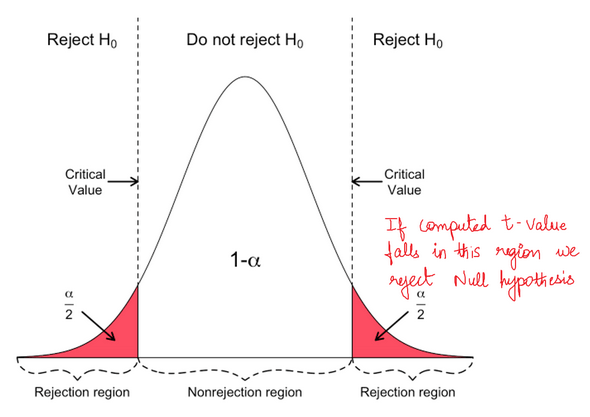
\includegraphics[width=0.7\textwidth]{figures/stats/one_side_t_test_rejection_regions.png}
\caption{
Illustration of a two-sided {\ttest}'s null hypothesis, $H_{0}$, rejection regions,
by \href{https://www.machinelearningplus.com/statistics/t-test-students-understanding-the-math-and-how-it-works/}{Selva Prabhakaran}.
In a one-sided \ttest we would only consider the side on a single side.
$\alpha$ is the significance level, typically \num{0.05} or lower.
}
\label{fig:two_sided_t_test}
\end{figure}

%%%%%%%%%%%%%%%%%%%%%%%%%%%%%%%%%%%%%%%%%%%%%%%%%%%%%%%%
\subsection{One-Sample}
\label{hypo:t_test:one}

In a one-sample \ttest we have one sample of size $n$ with mean $\expval{x}$ and standard deviation $s$,
and test $H_{0}$ that it belongs to a parent population with mean $\mu_{0}$.
In this case the parent population does not need to be normally distributed, but the distribution of possible $\expval{x}$ is assumed to be normal.

The \tstat \cref{eq:hypo:t:one} can be used with $\nu = n-1$ to find a \pvalue.

\begin{equation}\label{eq:hypo:t:one}
t = \frac{\expval{x} - \mu_{0}}{s / \sqrt{n}}
\end{equation}

%%%%%%%%%%%%%%%%%%%%%%%%%%%%%%%%%%%%%%%%%%%%%%%%%%%%%%%%
\subsection{Two-Sample: Unpaired}
\label{hypo:t_test:two:unpaired}

In a two-sample unpaired \ttest we have two independent samples, each of size $n$,
but with their own sample means $\expval{x_{i}}$ and standard deviations $s_{i}$.
Provided that we can assume that the two parent distributions of $x_{1}$ and $x_{2}$ have the same variance,
we can test $H_{0}$ that the two parent distribution means are equal.

The \tstat \cref{eq:hypo:t:two:unpaired} can be used with $\nu = 2n-2$ to find a \pvalue.

\begin{subequations}\label{eq:hypo:t:two:unpaired}
\begin{align}
t &= \frac{\expval{x_{1}} - \expval{x_{2}}}{s_{p} \sqrt{2/n}} \label{eq:hypo:t:two:unpaired:t} \\
s_{p} &= \sqrt{\left(s^{2}_{x_{1}} + s^{2}_{x_{2}}\right)/2} \label{eq:hypo:t:two:unpaired:s_p}
\end{align}
\end{subequations}

\subsubsection{Different Sample Sizes}
\label{hypo:t_test:two:unpaired:diff_n}

If we relax the sample size condition and let $n_{1} \neq n_{2}$
we can still compute a \tstat,
provided the parent distribution's variances are equal\footnote{A useful guideline is $1/2 < s_{x_{1}} / s_{x_{2}} < 2$.}.

The \tstat \cref{eq:hypo:t:two:unpaired:diff_n} can be used with $\nu = n_{1} + n_{2} - 2$ to find a \pvalue.

\begin{subequations}\label{eq:hypo:t:two:unpaired:diff_n}
\begin{align}
t &= \frac{\expval{x_{1}} - \expval{x_{2}}}{s_{p} \sqrt{\frac{1}{n_{1}} + \frac{1}{n_{2}}}} \label{eq:hypo:t:two:unpaired:diff_n:t} \\
s_{p} &= \sqrt{\left(\left(n_{1} - 1\right)s^{2}_{x_{1}} + \left(n_{2} - 1\right)s^{2}_{x_{2}}\right)/\left(n_{1} + n_{2} -2\right)} \label{eq:hypo:t:two:unpaired:diff_n:s_p}
\end{align}
\end{subequations}

\subsubsection{Different Sample Sizes and Variances (Welch's \texorpdfstring{$t$}{t}-Test)}
\label{hypo:t_test:two:unpaired:diff_n_diff_var}

If we further relax the assumptions and also let the population variances differ
we arrive at Welch's \ttest which approximates\footnote{The
true distribution of $t$ depends somewhat on the unknown population variances,
see the \href{https://en.wikipedia.org/wiki/Behrens\%E2\%80\%93Fisher_problem}{Behrens--Fisher problem}
for more.} the \tdist.

The \tstat \cref{eq:hypo:t:two:unpaired:diff_n_diff_var:t} can be used with $\nu$ \cref{eq:hypo:t:two:unpaired:diff_n_diff_var:dof} to find a \pvalue.

\begin{subequations}\label{eq:hypo:t:two:unpaired:diff_n_diff_var}
\begin{align}
t &= \frac{\expval{x_{1}} - \expval{x_{2}}}{\sqrt{\frac{s^{2}_{1}}{n_{1}} + \frac{s^{2}_{2}}{n_{2}}}} \label{eq:hypo:t:two:unpaired:diff_n_diff_var:t} \\
\nu &= \frac{\left(s^{2}_{1}/n_{1} + s^{2}_{2}/n_{2}\right)^{2}}{\frac{\left(s^{2}_{1}/n_{1}\right)^{2}}{n_{1}-1} + \frac{\left(s^{2}_{2}/n_{2}\right)^{2}}{n_{2}-1}} \label{eq:hypo:t:two:unpaired:diff_n_diff_var:dof}
\end{align}
\end{subequations}

%%%%%%%%%%%%%%%%%%%%%%%%%%%%%%%%%%%%%%%%%%%%%%%%%%%%%%%%
\subsection{Two-Sample: Paired}
\label{hypo:t_test:two:paired}

In a two-sample paired \ttest we have two dependent samples,
such as two sets of measurements from the same $n$ individuals taken at different times.
In this case, we are testing $H_{0}$ that the difference in means of the two dependent samples is $\mu_{0}$.
Note, we can set $\mu_{0} = 0$ if we simply want to test for a statistically significant difference, and not an \apriori degree of difference.
Defining the difference between paired observations as $x_{\Delta}$, we compute the mean difference $\expval{x_{\Delta}}$ and $s_{\Delta}$ standard deviation on the sample.

The \tstat \cref{eq:hypo:t:two:paired} can be used with $\nu = n-1$ to find a \pvalue.

\begin{equation}\label{eq:hypo:t:two:paired}
t = \frac{\expval{x_{\Delta}} - \mu_{0}}{s_{\Delta} / \sqrt{n}}
\end{equation}

%%%%%%%%%%%%%%%%%%%%%%%%%%%%%%%%%%%%%%%%%%%%%%%%%%%%%%%%
%%%%%%%%%%%%%%%%%%%%%%%%%%%%%%%%%%%%%%%%%%%%%%%%%%%%%%%%
\section{\texorpdfstring{$\chi^{2}$-Test}{Chi-Squared Test}}
\label{hypo:chi2_test}

Pearson's \chiSqtest can be used to
statistically compare a set of observations in
$n$ variables, $x_{i}$, to prior expectations via the \chiSqdist.
The \pvalue returned by the test estimates the probability of obtaining the observations
assuming $H_{0}$, \ie the expectations, is true.
The \chiSqstat, $X^{2}$, is created with the assumption that
the data are normally distributed and independent,
which often is the case due to the CLT.
It is constructed by squaring the difference\footnote{Yates's
correction for continuity $\left(x^{\text{obs}}_{j} - x^{\text{exp}}_{j}\right)^{2} \to \left(\abs{x^{\text{obs}}_{j} - x^{\text{exp}}_{j}}-0.5\right)^{2}$ may
also be applied in some low statistics cases.} between
an expected value, $x^{\text{exp}}_{i}$, and its corresponding observation, $x^{\text{obs}}_{i}$,
and dividing by the expectation:

\begin{equation}\label{eq:hypo:chi2_statistic}
X^{2} = \sum_{i=1}^{n} \frac{\left(x^{\text{obs}}_{i} - x^{\text{exp}}_{i}\right)^{2}}{x^{\text{exp}}_{i}}\,.
\end{equation}

In the limit that each $x^{\text{obs}}_{i}$ is normally distributed and $n$ is large, $X^{2} \to \chi^{2}$.
We can then use the \chiSqdist with $\nu = n-1$ degrees of freedom to find the \pvalue as the area to the right of $X^{2}$.
An easy way to compute $X^{2}$ and the \pvalue is to use the \texttt{scipy.stats.chisquare(f\_obs, f\_exp)}
\href{https://docs.scipy.org/doc/scipy/reference/generated/scipy.stats.chisquare.html}{function}.

The \chiSqtest can also be used to test of the data's independence, or homogeneity,
for $m$ samples of $n$ variables with $\nu = \left(n-1\right)\left(m-1\right)$ and\footnote{Note this is really the same as \cref{eq:hypo:chi2_statistic} if we reindex, just with a different $\nu$.}

\begin{equation}\label{eq:hypo:chi2_statistic_ind}
X^{2} = \sum_{i=1}^{n} \sum_{j=1}^{m} \frac{\left(x^{\text{obs}}_{i,j} - x^{\text{exp}}_{i,j}\right)^{2}}{x^{\text{exp}}_{i,j}}\,.
\end{equation}

%%%%%%%%%%%%%%%%%%%%%%%%%%%%%%%%%%%%%%%%%%%%%%%%%%%%%%%%
%%%%%%%%%%%%%%%%%%%%%%%%%%%%%%%%%%%%%%%%%%%%%%%%%%%%%%%%
\section{Analysis of Variance (ANOVA)}
\label{hypo:ANOVA}

When we are tasked with testing for differences between multiple groups
we should not use multiple pairwise tests, like two-sample unpaired {\ttest}s,
as the family-wise error rate \cref{eq:hypo:alpha_fw}
will compound and become unreasonable, see \cref{hypo:bonferroni_correction} for more.
Instead when dealing with three\footnote{When there are only two groups a one-factor ANOVA is equivalent to a two-sample unpaired \ttest with $F=t^{2}$.} or more groups
the appropriate Analysis of Variance (ANOVA) method should be used.
Like pairwise tests, there are multiple versions of ANOVA available for different situations, including
factorial ANOVA for multiple independent variables with interaction terms,
repeated measures ANOVA where the same subjects tested in different situations form the different groups,
Multivariate Analysis of Variance (MANOVA) for multiple dependent variables,
and further extensions such as Analysis of Covariance (ANCOVA) which incorporate correlations with additional covariate variables.
All share similar principles and assumptions,
but we will only focus on one-factor ANOVA here.

In general, ANOVA methods work by ``partitioning the sum of squares'',
\ie dividing the variance present in the data into
``explained variance'', \ie ``between-group variability'',
and
``unexplained variance'', \ie ``within-group variability'',
components.
The ratio of these components then form a \Fstat
which can be compared against the \Fdist
with the appropriate degrees of freedom to produce a \pvalue.
The null hypothesis $H_{0}$ is typically that all of the groups come from populations which share the same mean.
Increased between-group variability, or decreased within-group variability,
will increase the \Fstat and make rejecting $H_{0}$ more probable.
One downside to ANOVA testing is that if we reject $H_{0}$
we will not know which group(s) differ from the others.
In this case additional \posthoc analysis is required,
such as Bonferroni corrected {\ttest}s or Tukey's honest significance test.

%%%%%%%%%%%%%%%%%%%%%%%%%%%%%%%%%%%%%%%%%%%%%%%%%%%%%%%%
\subsection{Assumptions}
\label{hypo:ANOVA:assumptions}

Mathematically ANOVA is a special case of linear regression
and shares many of the same assumptions:

\begin{enumerate}[noitemsep]
  \item The variances of the different groups are equal (homoscedasticity).
  \item The observations $y_{ij}$ within group $i$ are independent and identically distributed (\iid) normal random variables.
  \item The residuals are normally distributed (normality\footnote{The normality assumption can be bent without severe consequences, but as always review the literature for specifics first.}).
  \item The dependent variable is continuous.
\end{enumerate}

%%%%%%%%%%%%%%%%%%%%%%%%%%%%%%%%%%%%%%%%%%%%%%%%%%%%%%%%
\subsection{One-Factor}
\label{hypo:ANOVA:one}

A one-factor ANOVA should be used when comparing $K$ groups,
divided by a single independent variable $x$,
across a single dependent variable $y$.
We partition the sum of squares into
mean square $MS_{\text{between-group}}$ and $MS_{\text{within-group}}$
\cref{eq:hypo:ANOVA:one:MS_between,eq:hypo:ANOVA:one:MS_within}, where
$n_{i}$ represents the number of observations in the $i$th group,
$N = \sum_{i} n_{i}$ is the total number of observations,
$y_{ij}$ is the $j$th observation for group $i$,
$\expval{Y_{i}} = \sum_{j} y_{ij} / n_{i}$ is the mean for group $i$,
and $\expval{Y} = \sum_{i}\sum_{j} y_{ij} / N$ is the overall mean across all groups.

\begin{subequations}\label{eq:hypo:ANOVA:one}
\begin{align}
MS_{\text{between-group}} &= \frac{1}{K-1} \sum_{i=1}^{K} n_{i}\left(\expval{Y_{i}} - \expval{Y}\right)^{2}, \label{eq:hypo:ANOVA:one:MS_between} \\
MS_{\text{within-group}} &= \frac{1}{N-K} \sum_{i=1}^{K} \sum_{j=1}^{n_{i}} \left( y_{ij} - \expval{Y_{i}} \right)^{2}, \label{eq:hypo:ANOVA:one:MS_within} \\
F &= \frac{MS_{\text{between-group}}}{MS_{\text{within-group}}}, \label{eq:hypo:ANOVA:one:F} \\
d_{1} &= K-1,\quad d_{2} = N-K. \label{eq:hypo:ANOVA:one:dof}
\end{align}
\end{subequations}

Note that $MS_{\text{between-group}}$ is comparing the group means to the overall mean,
while $MS_{\text{within-group}}$ is comparing all of the data points to their respective group means.
The \Fstat is then the ratio of the mean squares \cref{eq:hypo:ANOVA:one:F},
which can be used with the appropriate degrees of freedom \cref{eq:hypo:ANOVA:one:dof}
and the \Fdist to produce a \pvalue.
Depending on the \pvalue and selected $\alpha$
we can accept or reject $H_{0}$,
\ie all of the groups share one mean.
The \texttt{scipy.stats.f\_oneway} \href{https://docs.scipy.org/doc/scipy/reference/generated/scipy.stats.f_oneway.html#scipy.stats.f_oneway}{function}
performs\footnote{See
\href{https://www.analyticsvidhya.com/blog/2020/06/introduction-anova-statistics-data-science-covid-python/}{here} and
\href{https://www.reneshbedre.com/blog/anova.html}{here}
for example implementations.} the one-factor ANOVA test.

%%%%%%%%%%%%%%%%%%%%%%%%%%%%%%%%%%%%%%%%%%%%%%%%%%%%%%%%
%%%%%%%%%%%%%%%%%%%%%%%%%%%%%%%%%%%%%%%%%%%%%%%%%%%%%%%%
\section{\texorpdfstring{$F$}{F}-Test of Equality of Variances}
\label{hypo:F_test_var}

We can test $H_{0}$ that the variances of two normally distributed samples are equal with a \Ftest.
Given two samples of sizes $n_{1}$ and $n_{2}$ with sample variances $s_{2}^{2} \leq s_{1}^{2}$
we construct the \Fstat as:

\begin{equation}\label{eq:hypo:F_test_var}
F = \frac{s_{1}^{2}}{s_{2}^{2}}\,.
\end{equation}

The \Fdist with degrees of freedom $d_{1} = n_{1}-1$ and $d_{2} = n_{2}-1$
then gives an appropriate \pvalue.
Note that this \Ftest is particularly sensitive to the assumption that
the underlying samples are truly normally distributed;
not only approximately normal via the CLT.

%%%%%%%%%%%%%%%%%%%%%%%%%%%%%%%%%%%%%%%%%%%%%%%%%%%%%%%%
%%%%%%%%%%%%%%%%%%%%%%%%%%%%%%%%%%%%%%%%%%%%%%%%%%%%%%%%
\section{\texorpdfstring{$F$}{F}-Test of Lack-of-Fit Sum of Squares}
\label{hypo:F_test_fit}
% TODO

%%%%%%%%%%%%%%%%%%%%%%%%%%%%%%%%%%%%%%%%%%%%%%%%%%%%%%%%
%%%%%%%%%%%%%%%%%%%%%%%%%%%%%%%%%%%%%%%%%%%%%%%%%%%%%%%%
\section{Binomial Proportion Test}
\label{hypo:binomial_test}

When dealing with samples of $n$ binary events we can perform hypothesis testing
on the number of observed positive events $k$
using test statistics built on the binomial distribution.

%%%%%%%%%%%%%%%%%%%%%%%%%%%%%%%%%%%%%%%%%%%%%%%%%%%%%%%%
\subsection{Exact Binomial Test}
\label{hypo:binomial_test:exact}

For small $n$ it is possible to compute the \pvalue
explicitly from the binomial distribution \cref{eq:stats:binomial}.
We test $H_{0}$ that the probability of success is $\pi_{0}$
having actually observed $k$ successes, $k = n \pi$.

The \pvalue is then the sum

\begin{equation}\label{eq:hypo:binomial_test:exact}
\pvalue = \sum_{i \in \, \mathcal{I}} \binom{n}{i} \pi_{0}^{i} \left(1-\pi_{0}\right)^{n-i},
\end{equation}

\noindent where $\mathcal{I}$ depends on the type of test:

\begin{table}[H]
\centering
\begin{tabular}{l|l}
$\pi < \pi_{0}$ & $\mathcal{I} = \left\{0, 1, \ldots, k\right\}$, \\
$\pi > \pi_{0}$ & $\mathcal{I} = \left\{k, k+1, \ldots, n\right\}$, \\
$\pi \neq \pi_{0}$ & $\mathcal{I} = \left\{\forall \, i: P\left(x=i\right) \leq P\left(x = k\right)\right\}$, with binomial $P\left(x\right)$ \cref{eq:stats:binomial}.
\end{tabular}
\end{table}

%%%%%%%%%%%%%%%%%%%%%%%%%%%%%%%%%%%%%%%%%%%%%%%%%%%%%%%%
\subsection{One-Sample}
\label{hypo:binomial_test:one}

For large sample sizes the binomial distribution is approximated by the normal distribution
and we can use a form of the \Ztest to produce {\pvalue}s.
We require the observations to be independent,
\ie we may only sample $< \SI{10}{\percent}$ of the parent population,
the sampling distribution of $\pi$ to be approximately normal,
and that there are $\geq 10$ successes and $\geq 10$ failures,
$n \pi_{0} \geq 10$ and $n \left(1-\pi_{0}\right) \geq 10$, \ie the success-failure condition.

The \Zscore is then:

\begin{equation}\label{eq:hypo:binomial_test:one}
Z = \frac{\pi - \pi_{0}}{\sqrt{\pi_{0}\left(1-\pi_{0}\right)/n}} = \frac{k - n \pi_{0}}{\sqrt{n\pi_{0}\left(1-\pi_{0}\right)}}.
\end{equation}

Note that the one-sample test is provided by the
\texttt{scipy.stats.binomtest} \href{https://docs.scipy.org/doc/scipy/reference/generated/scipy.stats.binomtest.html}{function}.

%%%%%%%%%%%%%%%%%%%%%%%%%%%%%%%%%%%%%%%%%%%%%%%%%%%%%%%%
\subsection{Two-Sample}
\label{hypo:binomial_test:two}

In the case of two samples, we can test $H_{0}$
that the difference\footnote{Again, we set $\pi_{\Delta} = 0$ if we want to test for any difference.} in the sample's probabilities is $\pi_{\Delta}$.
We require that the $\pi$ from the two samples are uncorrelated,
have approximately normal sampling distributions,
and that their difference $\pi_{1} - \pi_{2}$ is an unbiased estimator.

The \Zscore is then:

\begin{subequations}\label{eq:hypo:binomial_test:two}
\begin{align}
Z &= \frac{\pi_{1} - \pi_{2} - \pi_{\Delta}}{\pi_{p} \left(1-\pi_{p}\right)\left(1/n_{1} + 1/n_{2}\right)} \label{eq:hypo:binomial_test:two:Z} \\
\pi_{p} &= \frac{k_{1} + k_{2}}{n_{1} + n_{2}} \label{eq:hypo:binomial_test:two:pi_p}
\end{align}
\end{subequations}

%%%%%%%%%%%%%%%%%%%%%%%%%%%%%%%%%%%%%%%%%%%%%%%%%%%%%%%%
%%%%%%%%%%%%%%%%%%%%%%%%%%%%%%%%%%%%%%%%%%%%%%%%%%%%%%%%
\section{Mann-Whitney \texorpdfstring{$U$}{U} Test}
\label{hypo:mann_whitney_U_test}
% TODO

%%%%%%%%%%%%%%%%%%%%%%%%%%%%%%%%%%%%%%%%%%%%%%%%%%%%%%%%
%%%%%%%%%%%%%%%%%%%%%%%%%%%%%%%%%%%%%%%%%%%%%%%%%%%%%%%%
\section{Kruskal-Wallis \texorpdfstring{$H$}{H} Test}
\label{hypo:kruskal_wallis_H_test}
% TODO

%%%%%%%%%%%%%%%%%%%%%%%%%%%%%%%%%%%%%%%%%%%%%%%%%%%%%%%%
%%%%%%%%%%%%%%%%%%%%%%%%%%%%%%%%%%%%%%%%%%%%%%%%%%%%%%%%
\section{Kolmogorov-Smirnov Test}
\label{hypo:KS_test}
% TODO

%%%%%%%%%%%%%%%%%%%%%%%%%%%%%%%%%%%%%%%%%%%%%%%%%%%%%%%%
%%%%%%%%%%%%%%%%%%%%%%%%%%%%%%%%%%%%%%%%%%%%%%%%%%%%%%%%
\section{Hypothesis Test Error Types and Power Analysis}
\label{hypo:power}

In hypothesis testing, like binary classification, we can suffer from two types of errors;
Type I or false positives, and Type II or false negatives.
The probabilities of these errors are functions of the experimental design
and are important to understand before undertaking a study.
We label $\alpha$ as the probability of rejecting a true null hypothesis, \ie a type I error,
and $\beta$ as the probability of failing to reject a false null hypothesis, \ie a type II error.
See \cref{table:CM} for a graphical representation in the context of binary classification.

$\alpha$ is the easier parameter to understand and improve,
as it is just the \pvalue threshold we select before the study.
It is typical to use $\alpha \leq \num{0.05}$.
$\beta$ depends on many factors including
$\alpha$,
the magnitude of the underlying effect,
the measurement variance,
the model being utilized,
and the sample size $n$.
Instead of using $\beta$ directly we often talk about the statistical power of a hypothesis test, $1-\beta$,
\ie the probability of correctly rejecting a false null hypothesis.
$\num{0.8} < 1-\beta$ is a commonly used target for the power.
As experimenters, we can
try to improve our methods to reduce the measurement variance,
select a more appropriate model\footnote{Parametric
models tend to have higher powers than the equivalent non-parametric model.
% https://youtu.be/diRX_NesFkA?t=558
In particular, comparing
the Mann-Whitney U and unpaired \ttest gives $\frac{\left(1-\beta\right)_{\text{MWU}}}{\left(1-\beta\right)_{t}} = \frac{3}{\pi} = \num{0.955}$,
%while comparing the Wilcoxon signed-rank and paired \ttest gives $\frac{\left(1-\beta\right)_{\text{WSR}}}{\left(1-\beta\right)_{t}} = \frac{2}{\pi} = \num{0.6437}$, % TODo add if I cover the Wilcoxon signed-rank test in the future
for large $n$.},
or begrudgingly accept some combination of a larger $\alpha$ or larger minimal detectable difference.
However, the primary lever for improving an experiment's power is by increasing $n$,
at the cost of additional time and money to complete the study.

%%%%%%%%%%%%%%%%%%%%%%%%%%%%%%%%%%%%%%%%%%%%%%%%%%%%%%%%
\subsection{\texorpdfstring{$Z$}{Z}-Test Power Example}
\label{hypo:power:Z_example}

Calculating $\beta$ can be challenging and is commonly done in software\footnote{The \texttt{statsmodels.stats.power}
\href{https://www.statsmodels.org/stable/stats.html\#power-and-sample-size-calculations}{module}
provides many useful functions, see \href{https://machinelearningmastery.com/statistical-power-and-power-analysis-in-python/}{here} for one example implementation.} particular to the model being utilized.
For a simple example, we can consider a \Ztest of a null hypothesis $\mu_{0}$
and compute the power of the test at a specific value of the alternative hypothesis $\mu_{a}$, with $\mu_{0} < \mu_{a}$.
For the given $\alpha$ being used we can look up the corresponding critical \Zscore, $Z_{\alpha}$.
Then assuming a standard deviation of $s_{\text{est}}$ from prior work,
and knowing $n$, we can estimate the sample mean
which would put us at the critical \Zscore, $\expval{x_{c}}$ \cref{eq:hypo:power_ex:x_c}.
We then calculate the \Zscore again, this time assuming the alternative hypothesis $\mu_{a}$ is true
and we have observed $\expval{x_{c}}$ from our sample, \ie we are right at the edge of rejecting a false null hypothesis.
This \Zscore, $Z_{a}$ \cref{eq:hypo:power_ex:Z_a}, can finally be used to find the power $1-\beta = P\left(Z_{a} < Z\right)$.

\begin{subequations}\label{eq:hypo:power_ex}
\begin{align}
Z_{\alpha} &= \frac{\expval{x_{c}} - \mu_{0}}{s_{\text{est}} / \sqrt{n}} \implies
\expval{x_{c}} = \frac{Z_{\alpha} s_{\text{est}}}{\sqrt{n}} + \mu_{0} \label{eq:hypo:power_ex:x_c} \\
Z_{a} &= \frac{\expval{x_{c}} - \mu_{a}}{s_{\text{est}} / \sqrt{n}}
= Z_{\alpha} + \sqrt{n}\,\frac{\mu_{0} - \mu_{a}}{s_{\text{est}}} \label{eq:hypo:power_ex:Z_a}
\end{align}
\end{subequations}

Note that as advertised $Z_{a}$ depends on
the choice of $\alpha$ via $Z_{\alpha}$,
the magnitude of the underlying effect $\mu_{0} - \mu_{a}$,
the measurement variance $s_{\text{est}}$,
the sample size $n$,
and is particular to this hypothesis test.
Plugging in numbers, if
$\alpha = \num{0.05} \to Z_{\alpha} = \num{1.645}$,
$\mu_{0} = \num{10}$,
$s_{\text{est}} \approx \num{2}$,
$n = \num{100}$,
and we want to find the power of the test for an alternative hypothesis of $\mu_{a} = \num{10.5}$,
we have $Z_{a} = \num{-0.8551} \to P\left(\num{-0.8551} < Z\right) = \num{0.8038}$
and thus the power is an acceptable $1-\beta = \num{0.8038} = \SI{80.38}{\percent}$.
We could use a similar line of reasoning to estimate
the $n$ necessary to obtain a desired $\alpha$ and $\beta$ before running the experiment.

% import numpy as np
% import scipy.stats
% norm = scipy.stats.norm
% Z_a = norm.ppf(1-0.05) + np.sqrt(100)*(10-10.5)/2
% print(f'Z_a = {Z_a:.4f}')
% print(f'Power = 1-beta = {1-norm.cdf(Z_a):.4f}')

%%%%%%%%%%%%%%%%%%%%%%%%%%%%%%%%%%%%%%%%%%%%%%%%%%%%%%%%
\subsection{Lehr's Equation for \texorpdfstring{$t$}{t}-Tests}
\label{hypo:power:lehr}

As a rough approximation for one-sided (two-sided) {\ttest}s,
Lehr argues that to have a power of $1-\beta \sim \num{0.8}$ with $\alpha = \num{0.05}$,
$n$ \cref{eq:hypo:power:lehr} should be set to 8\footnote{This
factor is $8 \approx \left(Z_{\alpha/2} + Z_{\beta}\right)^{2}$, for $1-\beta = \num{0.8}$, $\alpha = \num{0.05}$.} (16)
times the ratio of the estimated population variance, $s^{2}$,
and the desired detectable difference squared, $\Delta^{2} = \left(\mu_{1} - \mu_{2}\right)^{2}$.
Note that we can also rearrange this approximation to estimate $\Delta^{2}$ given a particular $n$.

\begin{subequations}\label{eq:hypo:power:lehr}
\begin{align}
n &\approx \hphantom{1}8 \frac{s^{2}}{\Delta^{2}}\quad \left(\text{One-Sided}\right), \label{eq:hypo:power:lehr:one} \\
n &\approx 16 \frac{s^{2}}{\Delta^{2}}\quad \left(\text{Two-Sided}\right). \label{eq:hypo:power:lehr:two}
\end{align}
\end{subequations}

%%%%%%%%%%%%%%%%%%%%%%%%%%%%%%%%%%%%%%%%%%%%%%%%%%%%%%%%
%%%%%%%%%%%%%%%%%%%%%%%%%%%%%%%%%%%%%%%%%%%%%%%%%%%%%%%%
\section{Bonferroni Correction}
\label{hypo:bonferroni_correction}

When conducting multiple hypothesis tests on the same set of data
we run the risk of underreporting $\alpha$ for the whole analysis.
In particle physics this is known as the look elsewhere effect\footnote{See the discussion in Appendix C of the dissertation \cite{mepland_dissertation}.}
\cite{Demortier:2007zz,lyons2008,Gross2010,Ranucci:2012ed}.
For example, if we set $\alpha = \num{0.05}$ for any individual test
on a set of data with many features, but then run $\num{20}$
tests on it, by chance we'd expect $\approx \num{1}$ tests
to erroneously reject a true $H_{0}$.
To quantify this concept, we can construct
the family-wise $\alpha$ across all of the $N$ tests done on a dataset\footnote{There is
disagreement on the best way to treat $\alpha_{\text{FW}}$,
\eg are we even talking about the right null hypothises \cite{Perneger1236},
what if the different tests are use correlated variables -- then they are not wholly independent tests in the context of $\alpha_{\text{FW}}$.
The $\alpha_{\text{FW}}$ of \cref{eq:hypo:alpha_fw} is just one simple definition.},
$\alpha_{\text{FW}}$ \cref{eq:hypo:alpha_fw}.
In our earlier example, we would have $\alpha_{\text{FW}} = \num{0.642}$,
or a \SI{64.2}{\percent} chance of at least one test rejecting $H_{0}$ in error.

\begin{equation}\label{eq:hypo:alpha_fw}
\alpha_{\text{FW}} = 1 - \left(1 - \alpha\right)^{N}
\end{equation}

To address this issue we can apply the Bonferroni correction,
and simply divide our nominal $\alpha$ by $N$
before conducting the tests\footnote{Or equivalently multiply the observed {\pvalue}s by $N$.}.

%%%%%%%%%%%%%%%%%%%%%%%%%%%%%%%%%%%%%%%%%%%%%%%%%%%%%%%%
\subsection{Sequential Bonferroni Correction, \texorpdfstring{\ie}{ie} Holm--Bonferroni Correction}
\label{hypo:bonferroni_correction:sequential}

We can control $\alpha_{\text{FW}}$ more efficiently in terms of the cost imposed on $\alpha$, and hence decreased power,
by using the sequential Bonferroni correction, \ie the Holm--Bonferroni correction.
As the name suggests, in the sequential correction
we iterate through the $i \in \left\{0, 1, \ldots, N-1\right\}$ tests
in order of their {\pvalue}s, from smallest to largest,
checking that $i$th test's \pvalue is $< \alpha / \left(N-i\right)$.
When we come to the first $i+1$ test with a $\pvalue \geq \alpha / \left(N-\left(i+1\right)\right)$
we stop iterating and say the previous $i$ tests reject $H_{0}$,
while the remaining $N-i$ tests fail to reject $H_{0}$.
In this way we can constrain $\alpha_{\text{FW}} \leq \alpha$,
while checking most tests against a less stringent condition
than $\alpha / N$ of the normal Bonferroni correction.

%%%%%%%%%%%%%%%%%%%%%%%%%%%%%%%%%%%%%%%%%%%%%%%%%%%%%%%%
%%%%%%%%%%%%%%%%%%%%%%%%%%%%%%%%%%%%%%%%%%%%%%%%%%%%%%%%
\section{Experiment Design}
\label{hypo:experiment}
% TODO

%%%%%%%%%%%%%%%%%%%%%%%%%%%%%%%%%%%%%%%%%%%%%%%%%%%%%%%%
\subsection{Sources of Bias}
\label{hypo:experiment:bias}
% TODO

%%%%%%%%%%%%%%%%%%%%%%%%%%%%%%%%%%%%%%%%%%%%%%%%%%%%%%%%
\subsection{Blocking}
\label{hypo:experiment:blocking}
% TODO

%%%%%%%%%%%%%%%%%%%%%%%%%%%%%%%%%%%%%%%%%%%%%%%%%%%%%%%%
\subsection{Interaction Effects}
\label{hypo:experiment:interaction}
% TODO

%%%%%%%%%%%%%%%%%%%%%%%%%%%%%%%%%%%%%%%%%%%%%%%%%%%%%%%%
\subsection{AB Testing Example}
\label{hypo:experiment:AB}
% TODO
}
%%%%%%%%%%%%%%%%%%%%%%%%%%%%%%%%%%%%%%%%%%%%%%%%%%%%%%%%
%%%%%%%%%%%%%%%%%%%%%%%%%%%%%%%%%%%%%%%%%%%%%%%%%%%%%%%%
\chapter{Regression}
\label{chap:regression}

%%%%%%%%%%%%%%%%%%%%%%%%%%%%%%%%%%%%%%%%%%%%%%%%%%%%%%%%
%%%%%%%%%%%%%%%%%%%%%%%%%%%%%%%%%%%%%%%%%%%%%%%%%%%%%%%%
\section{Linear Regression}
\label{regression:linear}

Linear regression fits the best hyperplane, or line in 1D,
to a collection of $m$ points $\mathbf{x}_{i}, y_{i}$,
typically via the method of least squares.
If $\mathbf{x}$ has $n$ features we can represent the
linear relationship between $\mathbf{x}$ and $y$ as:

\begin{equation}\label{eq:linear:onepoint}
y_{i} = \beta_{0} + \sum_{j=1}^{n}\, \beta_{j} x_{ij} + \epsilon_{i}\,,
\end{equation}

\noindent where $\beta_{j}$ are the parameters of the regression
and $\epsilon$ represent random errors.
Transitioning to matrix notation\footnote{Note
that \textit{linear} regression refers to the linearity in the model parameters
$\bm{\beta}$, not $\mathbf{X}$.
The components of $\mathbf{X}_{i}$ can be, and often are,
non-linear functions of other input features.}, this is simply:

\begin{equation}\label{eq:linear:matrix}
\mathbf{y} = \mathbf{X} \bm{\beta} + \bm{\epsilon}\,,
\end{equation}

\noindent where we have set $X_{i0} =1$.

The ordinary least squares (OLS) estimate of the parameters $\hat{\bm{\beta}}$
can be found by minimizing the squares of the residuals,
\ie the objective function $S\left(\bm{\beta}\right)$:

\begin{subequations} \label{eq:linear:ols}
\begin{align}
\hat{\bm{\beta}} &= \argmin_{\bm{\beta}} S\left(\bm{\beta}\right)\,, \label{eq:linear:argmin} \\
S\left(\bm{\beta}\right) &= \sum_{i=1}^{m} \, \abs{y_{i} - \sum_{j=0}^{n} \, \beta_{j} x_{ij}}^{2} = \norm{\mathbf{y} - \mathbf{X} \bm{\beta}}^{2}\,. \label{eq:linear:S}
\end{align}
\end{subequations}

\noindent The optimal $\hat{\bm{\beta}}$ of \cref{eq:linear:ols} has a closed form solution:

\begin{equation}\label{eq:linear:betahat}
\hat{\bm{\beta}} = \left(\mathbf{X}\transpose\mathbf{X}\right)^{-1}\mathbf{X}\transpose \mathbf{y}\,,
\end{equation}

\noindent provided the following assumptions hold:

%%%%%%%%%%%%%%%%%%%%%%%%%%%%%%%%%%%%%%%%%%%%%%%%%%%%%%%%
\subsection{Assumptions}
\label{regression:linear:assumptions}

\begin{enumerate}[noitemsep]
\item The underlying relationship between $\mathbf{x}$ and $y$ is linear, and there are no major outliers.\label{item:regression:linear:linear}
\item The columns of $\mathbf{X}$, \ie features, are linearly independent, \ie $\mathrm{rank}\left(\mathbf{X}\right) = n$ (no multicollinearity).\label{item:regression:linear:multicollinearity}
\item The errors $\epsilon$ have conditional mean 0, $E\left(\epsilon \mid \mathbf{X}\right) = 0$ (exogeneity). The errors thus:\label{item:regression:linear:exogeneity}
\begin{enumerate}[noitemsep]
\item Have a mean of zero, $E\left(\epsilon\right) = 0$.
\item Are not correlated with the input features, $E\left(\mathbf{X}\transpose\epsilon\right) = 0$.
\end{enumerate}
\item The errors are spherical, $\mathrm{var}\left(\epsilon \mid \mathbf{X}\right) = \sigma^{2} \identity$. Thus:\label{item:regression:linear:spherical}
\begin{enumerate}[noitemsep]
\item Each observation $\mathbf{x}_{i}$ has the same constant variance $\sigma^{2}$ (homoscedasticity).
\item The errors are uncorrelated between observations, $E\left(\epsilon_{i}\epsilon_{j \neq i} \mid \mathbf{X}\right) = 0$ (no autocorrelation).
\end{enumerate}
\item The errors are normally distributed (multivariate normality)\footnote{This is not strictly required, but if true the OLS is the MLE and hypothesis testing works.}.\label{item:regression:linear:normality}
\end{enumerate}

If these assumptions are violated the following issues arise,
namely the model may be biased and or have a large or invalid estimated variance\footnote{A good reference may be found \href{http://people.duke.edu/~rnau/testing.htm}{here}.}:

\begin{itemize}[noitemsep]
\item[\ref{item:regression:linear:linear}.] If you are fitting nonlinear data the predictions will have large errors,
particularly when extrapolated beyond the range of the fitted data.
This will show up as systematic errors in the residuals plot,
or may be obvious when comparing observed vs predicted values.
Possible fixes include applying a nonlinear transformation to some of the features to linearize the data, \eg take the log,
adding more combinations of features, \eg higher polynomial terms,
or finding new independent features which may explain the nonlinearity.

\item[\ref{item:regression:linear:multicollinearity}.] If some of the features are not linearly independent (multicollinearity),
they can be biasing the model and should be removed in turn until linear independence is restored.
Multicollinearity can be spotted in the input feature correlation matrix,
or if the residuals correlate to any of the features.

\item[\ref{item:regression:linear:exogeneity}. \& \ref{item:regression:linear:spherical}.] If something is wrong with the errors
such that they correlate to the input features or across observations\footnote{Thus the residuals correlate with row number, \ie autocorrelation.},
have a non-zero mean, or have a changing variance,
the reported confidence intervals on the model parameters may be over or underestimated.

\item[\ref{item:regression:linear:normality}.] If the errors are not normally distributed the confidence intervals are again suspect.
This can be diagnosed by comparing the errors to the normal distribution with a normal probability plot, or normal quantile plot,
or through a statistical method like the Anderson-Darling and Kolmogorov-Smirnov tests.
Note that violating normality in the errors is not as much of an issue compared to the other assumptions
since the fit will still give usable coefficients provided the assumed form of the model is correct.
Problems of this kind can arise from nonlinear data or influential outliers.
If the errors really are non-normal, a generalized linear model (GLM) could be employed to model them correctly.
\end{itemize}

%%%%%%%%%%%%%%%%%%%%%%%%%%%%%%%%%%%%%%%%%%%%%%%%%%%%%%%%
\subsection{Goodness of Fit}
\label{regression:linear:goodness_of_fit}

% TODO R2, reduced chi square values, F-test, t-test

% TODO Ridge regression
% TODO Lasso regression

%%%%%%%%%%%%%%%%%%%%%%%%%%%%%%%%%%%%%%%%%%%%%%%%%%%%%%%%
%%%%%%%%%%%%%%%%%%%%%%%%%%%%%%%%%%%%%%%%%%%%%%%%%%%%%%%%
\section{Logistic Regression}
\label{regression:logistic}

Logistic regression is a simple method to create a classifier,
typically on two classes $y = 0,1$, though multinomial extensions exist.
Its name comes from the use of the logit, or log-odds, function

\begin{equation}\label{eq:logistic:logic}
l = \text{logit}\left(p\right) = \log\left(\frac{p}{1-p}\right)
\end{equation}

\noindent on the probability $p$ of class $1$.
$l$ is estimated linearly from $n$ input features $x_{j}$ with $n+1$ parameters $\beta_{j}$ as:

\begin{equation}\label{eq:logistic:logicBeta}
l = \beta_{0} + \sum_{j=1}^{n} \, \beta_{j}\,x_{j}\,.
\end{equation}

\noindent The probability $p$ is then

\begin{equation}\label{eq:logistic:p}
p = \frac{e^l}{e^l + 1} = \frac{1}{1+e^{-l}} = \text{logit}^{-1}\left(l\right)
\end{equation}

\noindent which can be turned into a predicted class through the choice of a suitable decision threshold.

The model parameters $\bm{\beta}$ are chosen by maximizing
the log of the likelihood $L$ \cref{eq:logistic:L} over $m$ known example points $\mathbf{x}_{i}, y_{i}$.
Note that $P\left(y \mid x\right)$ \cref{eq:logistic:Pr} is simply the Bernoulli distribution.
In practice the log-likelihood $\log\left(L\right)$ is maximized via gradient descent.
An example of logistic regression can be found in \cref{fig:logistic_regression_ex}.

\begin{subequations} \label{eq:logistic:L_Pr}
\begin{align}
L\left(\bm{\beta} \mid \mathbf{x}\right) &= \prod_{i=1}^{m} \, P\left(y_{i} \mid \mathbf{x}_{i};\,\bm{\beta}\right) \label{eq:logistic:L} \\
P\left(y \mid \mathbf{x}\right) &= p^y\left(1-p\right)^{1-y}, \quad y \in \{0, 1\} \label{eq:logistic:Pr}
\end{align}
\end{subequations}

\begin{figure}
\centering
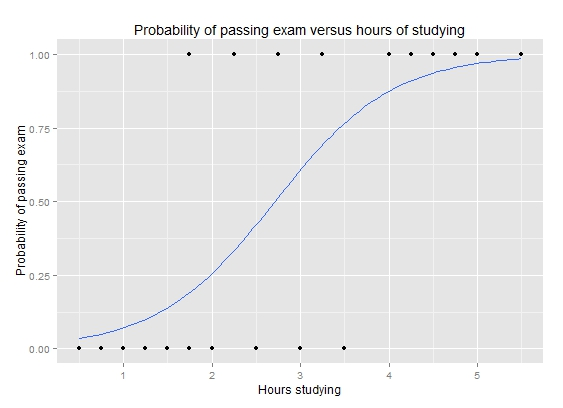
\includegraphics[width=0.8\textwidth]{figures/regression/Exam_pass_logistic_curve.jpeg}
\caption{
Example logistic regression curve on one input feature, by \href{https://en.wikipedia.org/wiki/File:Exam_pass_logistic_curve.jpeg}{Michaelg2015}.
}
\label{fig:logistic_regression_ex}
\end{figure}

Some assumptions of the logistic regression approach are:
\begin{enumerate}[noitemsep]
\item $y$ is either present or absent (dichotomous).
\item There are minimal correlations between the $x_{j}$ features (no multicollinearity).
\item There are no major outliers in the data.
\end{enumerate}

% TODO pseudo R2, Wald statistic

%%%%%%%%%%%%%%%%%%%%%%%%%%%%%%%%%%%%%%%%%%%%%%%%%%%%%%%%
%%%%%%%%%%%%%%%%%%%%%%%%%%%%%%%%%%%%%%%%%%%%%%%%%%%%%%%%
\section{Gaussian Process Regression}
\label{Regression:kriging}
% TODO also known as kriging

}
%%%%%%%%%%%%%%%%%%%%%%%%%%%%%%%%%%%%%%%%%%%%%%%%%%%%%%%%
%%%%%%%%%%%%%%%%%%%%%%%%%%%%%%%%%%%%%%%%%%%%%%%%%%%%%%%%
%%%%%%%%%%%%%%%%%%%%%%%%%%%%%%%%%%%%%%%%%%%%%%%%%%%%%%%%
\chapter{General Machine Learning Concepts}
\label{ml:general}

%%%%%%%%%%%%%%%%%%%%%%%%%%%%%%%%%%%%%%%%%%%%%%%%%%%%%%%%
%%%%%%%%%%%%%%%%%%%%%%%%%%%%%%%%%%%%%%%%%%%%%%%%%%%%%%%%
\section{Evaluating Performance}
\label{ml:general:eval}

%%%%%%%%%%%%%%%%%%%%%%%%%%%%%%%%%%%%%%%%%%%%%%%%%%%%%%%%
\subsection{Confusion Matrix}
\label{ml:general:eval:cm}

The confusion matrix is a simple table of the number of actual, or truth, class instances
versus the number of a model's predicted class instances.
A two class example is provided in \cref{table:CM}.
Multi-class confusion matrices are straight forward extensions,
with correctly classified instances appearing along the diagonal.

\begin{table}[H]
  \centering
  \begin{tabular}{c | c | c | c |}
  \multicolumn{2}{c}{} & \multicolumn{2}{c}{\textbf{Actual}} \\ \cline{3-4}
  \multicolumn{1}{c}{} & & Positive & Negative \\ \cline{2-4}
  \multirow{4}{*}{\rotatebox{90}{\textbf{Predicted}}} & \multirow{2}{*}{Positive} & \multirow{2}{*}{TP} & FP \\[-8pt]
   & & & (Type I) \\ \cline{2-4}
   & \multirow{2}{*}{Negative} & FN & \multirow{2}{*}{TN} \\[-8pt]
   & & (Type II) & \\ \cline{2-4}
  \end{tabular}
  \caption{Two class confusion matrix.}
  \label{table:CM}
\end{table}

%%%%%%%%%%%%%%%%%%%%%%%%%%%%%%%%%%%%%%%%%%%%%%%%%%%%%%%%
\subsection{TPR \& TNR -- Sensitivity \& Specificity}
\label{ml:general:eval:TPR_TNR}

The true positive rate (TPR) and true negative rate (TNR) are
relatively straight forward to compute and understand, along with their complements,
the false negative rate (FNR), \ie miss rate, and false positive rate (FPR), \ie fall-out.
Here the denominators are the number of true class members.

\begin{enumerate}[noitemsep]
\item True positive rate (TPR), \ie sensitivity, recall, hit rate:
\begin{equation} \label{eq:TPR}
\text{TPR} = \frac{\text{TP}}{\text{P}} = \frac{\text{TP}}{\text{TP}+\text{FN}} = 1 - \text{FNR} = P\left(\hat{+} \mid + \right)
\end{equation}

\item True negative rate (TNR), \ie specificity, selectivity:
\begin{equation} \label{eq:TNR}
\text{TNR} = \frac{\text{TN}}{\text{N}} = \frac{\text{TN}}{\text{TN}+\text{FP}} = 1 - \text{FPR} = P\left(\hat{-} \mid - \right)
\end{equation}
\end{enumerate}

%%%%%%%%%%%%%%%%%%%%%%%%%%%%%%%%%%%%%%%%%%%%%%%%%%%%%%%%
\subsection{PPV (Precision) \& NPV}
\label{ml:general:eval:PPV_NPV}

The positive predictive value (PPV), more commonly known as precision, and negative predictive value (NPV)
are related metrics, but with predicted class members in the denominators.
Their complements are the false discovery rate (FDR) and false omission rate (FOR).
It is helpful to look at these metrics graphically, as in \cref{fig:graphical_CM_quantities}.

\begin{enumerate}[noitemsep]
\item Positive predictive value (PPV), \ie precision:
\begin{equation} \label{eq:PPV}
\text{PPV} = \frac{\text{TP}}{\hat{\text{P}}} = \frac{\text{TP}}{\text{TP}+\text{FP}} = 1 - \text{FDR} = P\left(+ \mid \hat{+} \right)
\end{equation}

\item Negative predictive value (NPV):
\begin{equation} \label{eq:NPV}
\text{NPV} = \frac{\text{TN}}{\hat{\text{N}}} = \frac{\text{TN}}{\text{TN}+\text{FN}} = 1 - \text{FOR} = P\left(- \mid \hat{-} \right)
\end{equation}
\end{enumerate}

\begin{figure}[H]
\centering
  \begin{subfigure}[c]{0.48\textwidth}\centering
  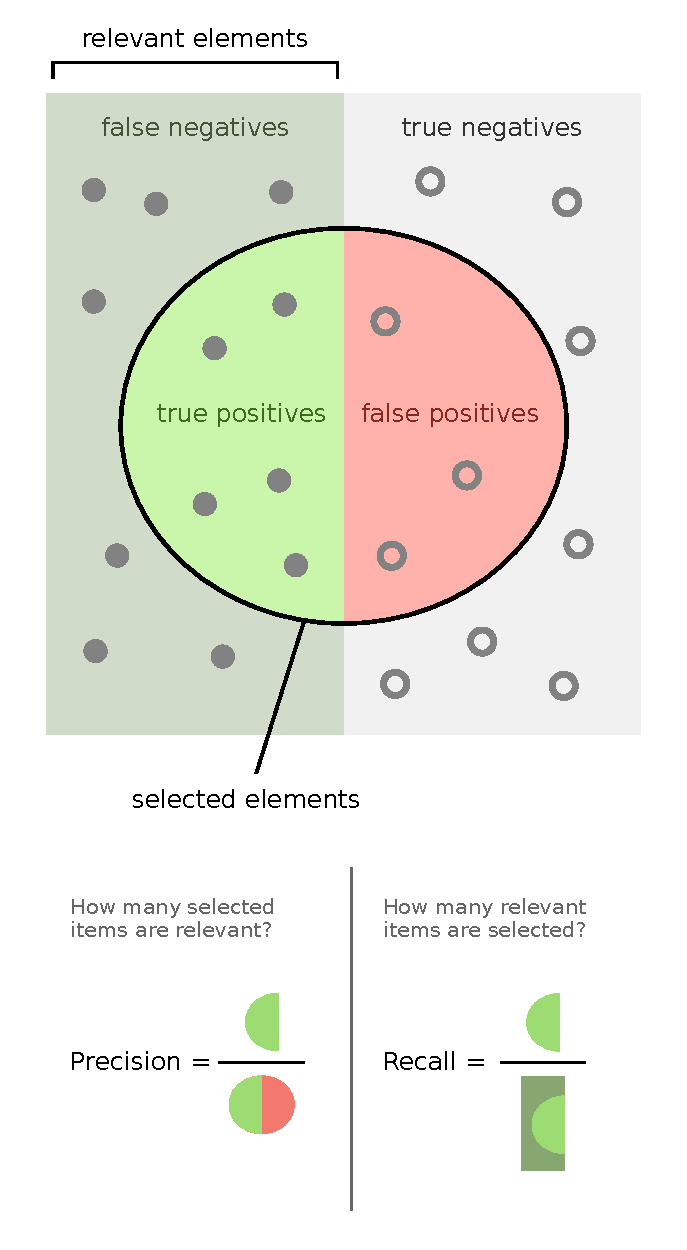
\includegraphics[width=\textwidth]{figures/ml/precision_recall.pdf}
  \caption{Precision \& Recall}
  \label{fig:graphical_CM_quantities:precision_recall}
  \end{subfigure}
  ~
  \begin{subfigure}[c]{0.48\textwidth}\centering
  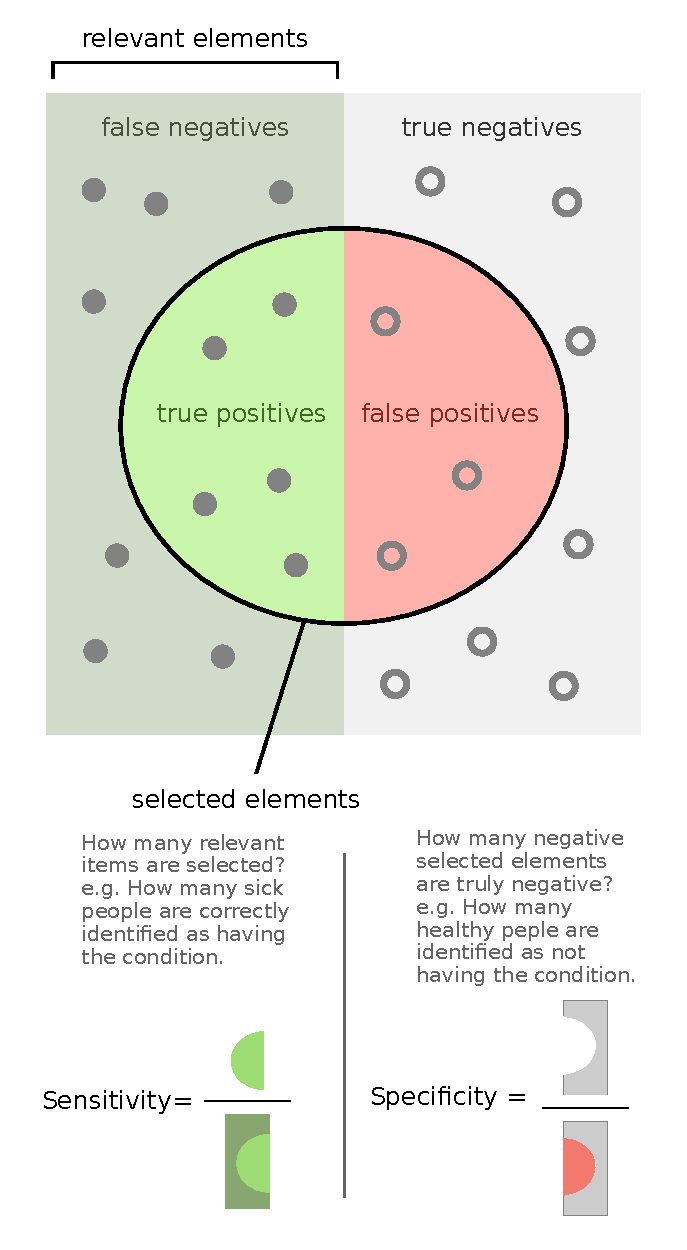
\includegraphics[width=\textwidth]{figures/ml/sensitivity_and_specificity.pdf}
  \caption{Sensitivity \& Specificity}
  \label{fig:graphical_CM_quantities:sensitivity_specificity}
  \end{subfigure}
\caption{
Graphical representation of
precision versus recall (sensitivity), by \href{https://commons.wikimedia.org/wiki/File:Precisionrecall.svg}{Walber},
and
sensitivity (recall) versus specificity, by \href{http://en.wikipedia.org/wiki/File:Sensitivity_and_specificity.svg}{FeanDoe}.
}
\label{fig:graphical_CM_quantities}
\end{figure}

%%%%%%%%%%%%%%%%%%%%%%%%%%%%%%%%%%%%%%%%%%%%%%%%%%%%%%%%
\subsection{Other Scores}
\label{ml:general:eval:other_scores}

The accuracy (ACC), the proportion of correct predictions, is a natural metric for measuring a classifiers performance.
Various F-scores, such as $F_{1}$ and $F_{\beta}$, combine precision and recall into one metric\footnote{Note that $F_{\beta}$ does not depend on TN at all, a potential shortcoming.}.
$F_{1}$ balances precision and recall equally, and is their harmonic mean,
while $F_{\beta}$ uses $\beta$ to assign different weights to each\footnote{$F_{2}$ weights recall over precision, $F_{0.5}$ weights precision over recall.}.

\begin{enumerate}[noitemsep]
\item Accuracy (ACC):
\begin{equation} \label{eq:ACC}
\text{ACC} = \frac{\text{TP}+\text{TN}}{\text{P}+\text{N}} = \frac{\text{TP}+\text{TN}}{\text{TP}+\text{TN}+\text{FP}+\text{FN}}
\end{equation}

\item $F_{1}$ ($F_{1}=1$ is best, $F_{1}=0$ is worst):
\begin{equation} \label{eq:F1}
F_{1} = \left(\frac{\text{precision}^{-1}+\text{recall}^{-1}}{2}\right)^{-1} = 2\,\,\frac{\text{precision} \times \text{recall}}{\text{precision} + \text{recall}}
\end{equation}

\item $F_{\beta}$ (Larger $\beta$ weights recall over precision):
\begin{equation} \label{eq:Fbeta}
F_{\beta} = \left(1+\beta^{2}\right) \frac{\text{precision} \times \text{recall}}{\beta^{2}\,\text{precision} + \text{recall}} =
\frac{\left(1+\beta^{2}\right) \text{TP}}{\left(1+\beta^{2}\right) \text{TP} + \beta^{2}\,\text{FN} + \text{FP}}
\end{equation}
\end{enumerate}

\clearpage% TODo hard coded
%%%%%%%%%%%%%%%%%%%%%%%%%%%%%%%%%%%%%%%%%%%%%%%%%%%%%%%%
%%%%%%%%%%%%%%%%%%%%%%%%%%%%%%%%%%%%%%%%%%%%%%%%%%%%%%%%
\section{Bias-Variance Tradeoff}
\label{ml:general:bias_variance_tradeoff}

\begin{enumerate}[noitemsep]
\item Bias: Errors due to a model not learning about relationships between features in the training data, \ie underfitting. Caused by invalid relationships present in the model.
\item Variance: Errors due to an overly complex model failing to generalize beyond the training data, \ie overfitting. Caused by sensitivity to small fluctuations in the training data.
\end{enumerate}

\begin{figure}[H]
  \centering
  \savebox{\largestimage}{
    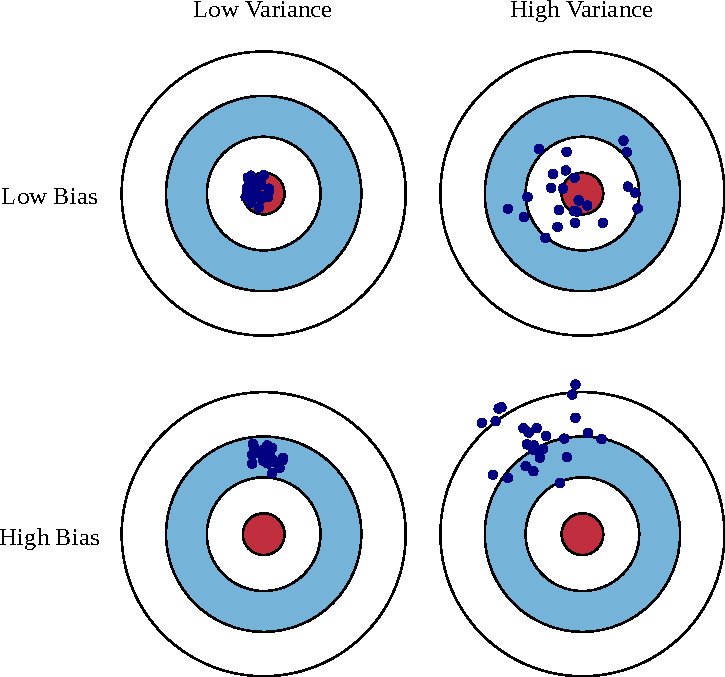
\includegraphics[width=0.47\textwidth]{figures/ml/bias_variance_tradeoff.pdf}
  }% Store largest image in a box

  \begin{subfigure}[b]{0.48\textwidth}\centering
    \usebox{\largestimage}
    \vspace{0.01cm}
  \caption{Direct Comparison}
  \label{fig:ml:bias_variance_tradeoff:direct}
  \end{subfigure}
  ~
  \begin{subfigure}[b]{\wd\largestimage}\centering
    \raisebox{\dimexpr.5\ht\largestimage-.5\height}{% Adjust vertical height of smaller image
      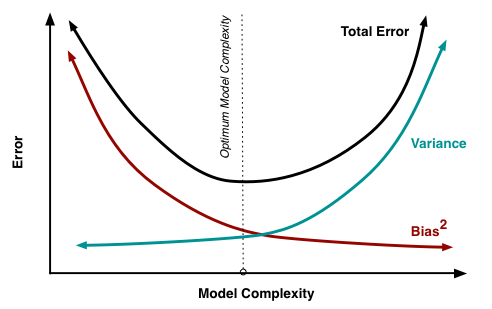
\includegraphics[width=\textwidth]{figures/ml/bias_variance_error_tradeoff.png}}
  \caption{Error Components (Test Set)}
  \label{fig:ml:bias_variance_tradeoff:error}
  \end{subfigure}
\caption{
Illustrations of the bias-variance tradeoff,
by \href{http://scott.fortmann-roe.com/docs/BiasVariance.html}{Scott Fortmann-Roe}.
\label{fig:ml:bias_variance_tradeoff}
}
\end{figure}

Every model makes a tradeoff between bias and variance,
which is roughly controlled by its level of complexity
as can be seen in \cref{fig:ml:bias_variance_tradeoff:error}.
\Cref{fig:additional:ml:general:early_stopping} shows this in practice,
as past a certain point of complexity the validation error grows
while the training error continues to decrease.

\subsubsection{Mean Square Error (MSE) Decomposition}
\label{ml:general:bias_variance_tradeoff:decop}

We can analytically decompose the mean square error (MSE) into explicit
bias, variance, and irreducable error components.
Let $y = f\left(\mathbf{x}\right) + \epsilon$ represent
the observed data, $y_{i}$, $\mathbf{x}_{i}$,
where $f\left(\mathbf{x}\right)$ is the true parent distribution\footnote{$\expval{f} = f$ is deterministic,
and acts as a constant as far as expectation values are concerned.} and
$\epsilon$ is random noise\footnote{This is the source of the irreducible error.
Since future data will still have $\epsilon$, the predictions can't be perfect
-- even when neglecting the model's own bias and variance.}\footnote{Later we'll need
$\sigma^{2} = \variance{\epsilon} = \expval{\epsilon^{2}} - \expval{\epsilon}^{2} = \expval{\epsilon^{2}}$.} having
$\expval{\epsilon} = 0$, $\variance{\epsilon} = \sigma^{2}$.
Representing the trained model\footnote{Note
that $\cov{\epsilon}{\hat{f}} = 0 \Rightarrow \expval{\epsilon \hat{f}} = \expval{\epsilon} \expval{\hat{f}}$.} as
$\hat{f}\left(\mathbf{x}\right)$, we expand the MSE:

\begin{subequations} \label{eq:bias_variance_tradeoff:decop}
\begin{align}
\text{MSE} &= \expval{\left(y-\hat{f}\right)^{2}} \\
&= \expval{\left(f + \epsilon - \hat{f} + \big[\expval{\hat{f}}-\expval{\hat{f}}\big]\right)^{2}}\,, \\
&= \expval{\left(\big[f - \expval{\hat{f}}\big] + \epsilon - \big[\hat{f} - \expval{\hat{f}}\big]\right)^{2}}\,, \\
&= \expval{\left(f-\expval{\hat{f}}\right)^{2}}
+\expval{\epsilon^{2}}
+\expval{\left(\hat{f}-\expval{\hat{f}}\right)^{2}}
+2\expval{\left(f-\expval{\hat{f}}\right)\epsilon} \\
&\hphantom{=}-2\expval{\epsilon\left(\hat{f}-\expval{\hat{f}}\right)}
-2\expval{\left(f-\expval{\hat{f}}\right)\left(\hat{f}-\expval{\hat{f}}\right)}\,, \\
&= \left(-1\right)^{2}\left(\expval{\hat{f}}-f\right)^{2} +\sigma^{2} + \variance{\hat{f}}
+2\left(f-\expval{\hat{f}}\right)\cancelto{0}{\expval{\epsilon}} \\
&\hphantom{=}-2\cancelto{0}{\expval{\epsilon}}\left(\expval{\hat{f}}-\expval{\hat{f}}\right)
-2\left(f-\expval{\hat{f}}\right)\cancelto{0}{\left(\expval{\hat{f}}-\expval{\hat{f}}\right)}\,, \\
&= \left(\bias{\hat{f}}\right)^{2} + \variance{\hat{f}} + \sigma^{2}\,.
\end{align}
\end{subequations}

\clearpage% TODo hard coded
%%%%%%%%%%%%%%%%%%%%%%%%%%%%%%%%%%%%%%%%%%%%%%%%%%%%%%%%
%%%%%%%%%%%%%%%%%%%%%%%%%%%%%%%%%%%%%%%%%%%%%%%%%%%%%%%%
\section{Regularization}
\label{ml:general:reg}

Regularization is a method for controlling the variance (overfitting)
of a model by putting constraints on the size of its parameters.
In terms of \cref{ml:general:bias_variance_tradeoff}, regularization forces the model's
bias to grow on the training set in order to lower the variance on future data.
The two main types of regularization are shown in \cref{eq:L1_L2}
and depend on different powers of the norm\footnote{In
the case of OLS linear regression the constant intercept term $\beta_{0}$ is not included in $\norm{\bm{\beta}}$.} of the model parameters $\bm{\beta}$.
In order to treat all features equally, normalization must be used before applying regularization.
A hyperparameter $\lambda$ is included to tune the amount of regularization applied in the objective function,
$S\left(\bm{\beta}\right) = L + \Omega$.
As $\lambda$ is increased, it decreases the size the model's coefficients, and thereby its variance (overfitting),
up to a point when the model is unable to adequately train on the available data and the bias (underfitting) begins to grow.

\begin{subequations} \label{eq:L1_L2}
\begin{align}
\Omega_{\text{L1}}\left(\bm{\beta}\right) &= \lambda \norm{\bm{\beta}}\hphantom{^{1}}
= \lambda \sum_{j=1}^{n} \, \abs{\beta_{j}}\,, \label{eq:L1} \\
\Omega_{\text{L2}}\left(\bm{\beta}\right) &= \lambda \norm{\bm{\beta}}^{2}
= \lambda \sum_{j=1}^{n} \,\, \beta_{j}^{2}\,. \label{eq:L2}
\end{align}
\end{subequations}

For a particular value of $\lambda$, the effect of L1 and L2 regularization\footnote{Here
$q$ is being used as the power of $\norm{\bm{\beta}}$. For L1 (L2), $q=1$ ($q=2$).} is
to constrain $\norm{\bm{\beta}}^{q} \leq t\left(\lambda\right)$ for some $t\left(\lambda\right)$.
As can be seen in \cref{fig:ml:l1l2} the L1 norm constrains $\bm{\beta}$ to lie within a hypercube,
while the L2 constraint is a hypersphere.

\begin{figure}[H]
  \centering
  \begin{subfigure}[b]{0.48\textwidth}\centering
      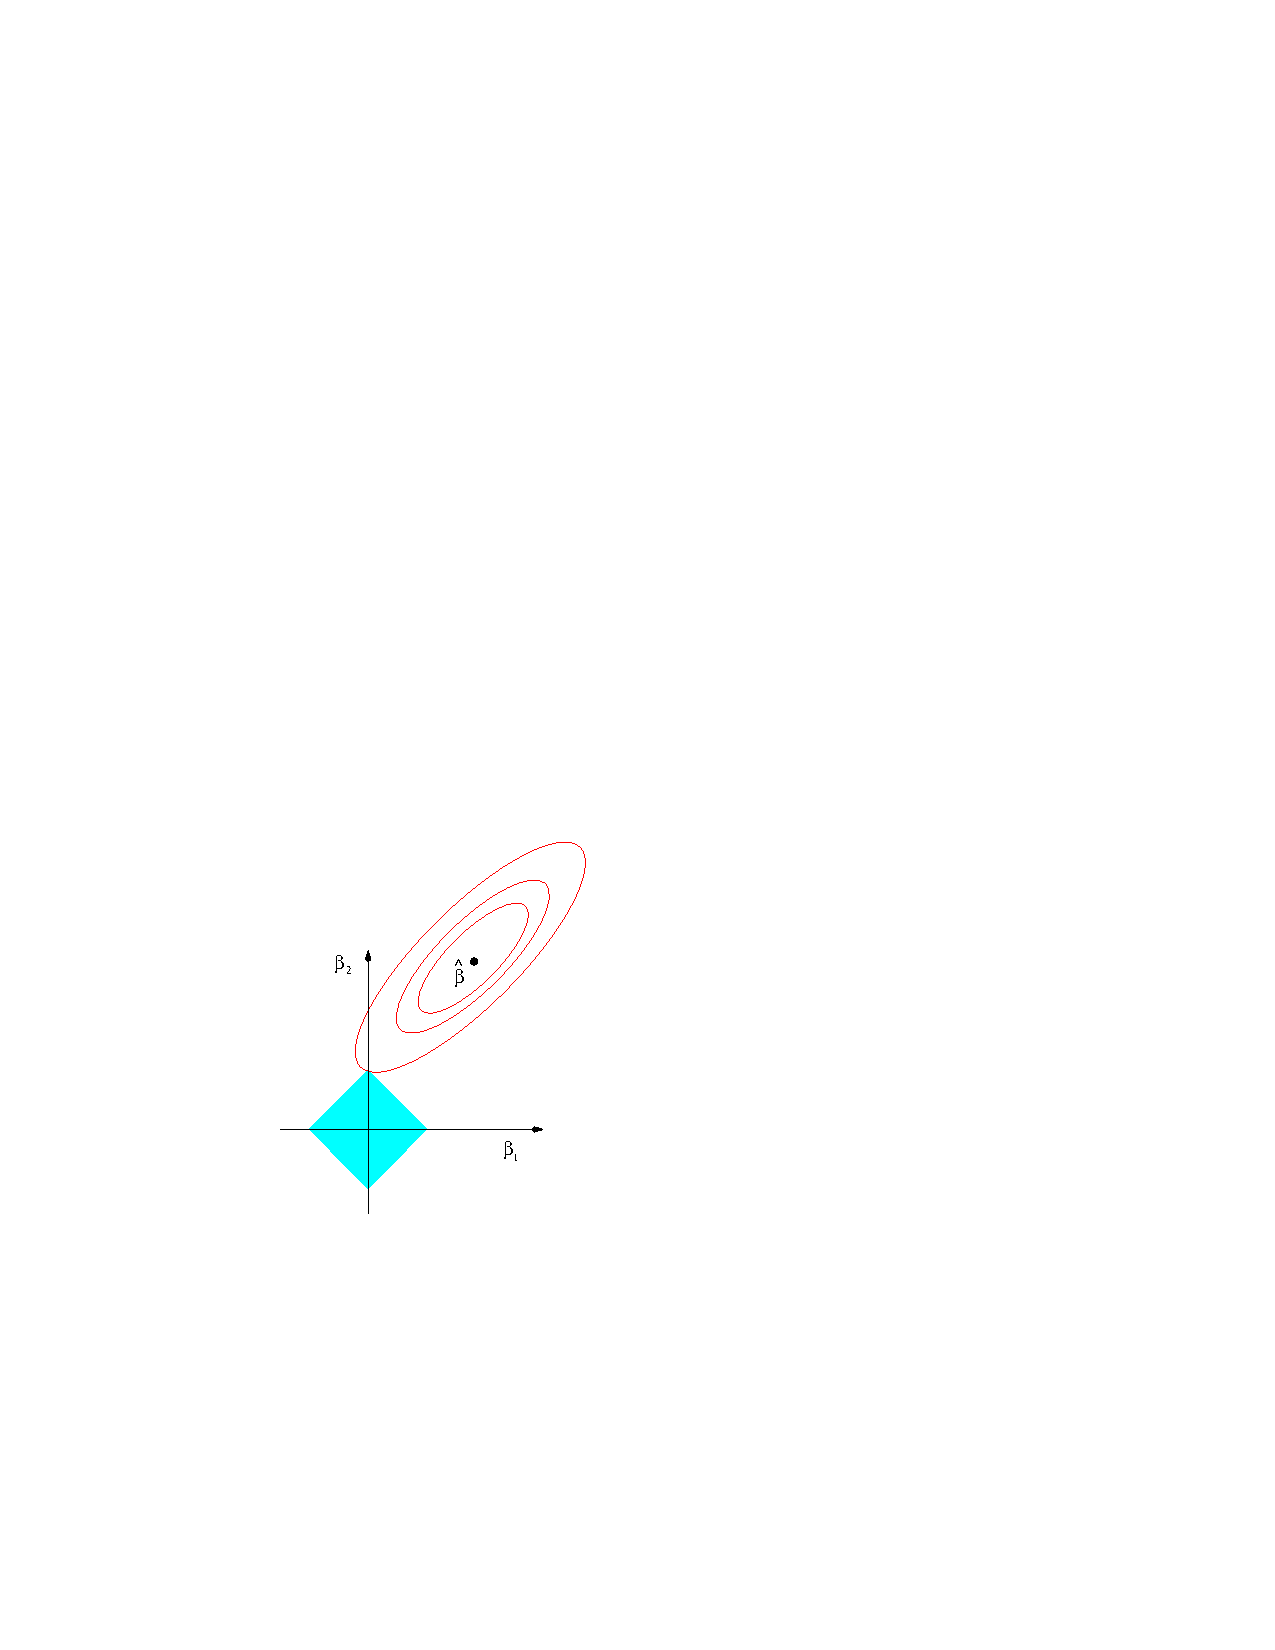
\includegraphics[width=\textwidth]{figures/ml/l1.pdf}
  \caption{L1}
  \label{fig:ml:l1l2:l1}
  \end{subfigure}
  ~
  \begin{subfigure}[b]{0.48\textwidth}\centering
      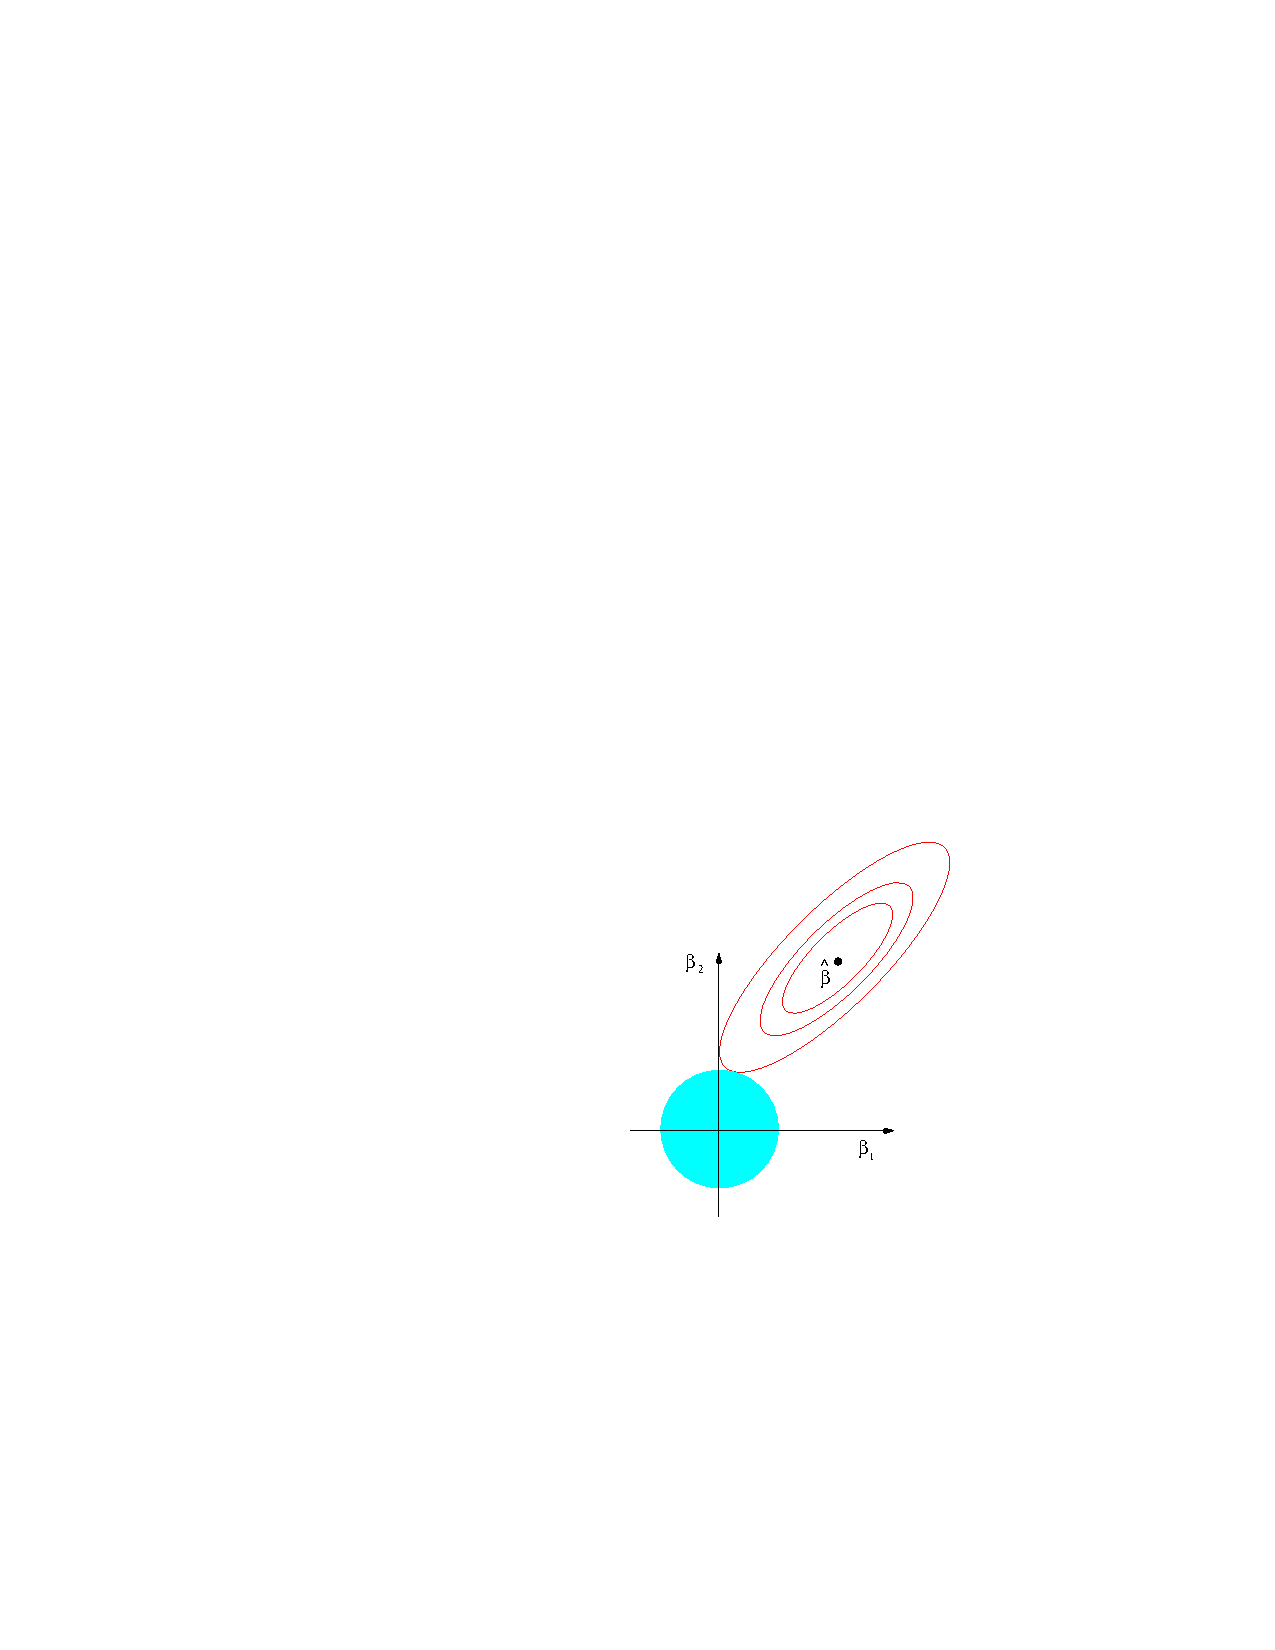
\includegraphics[width=\textwidth]{figures/ml/l2.pdf}
  \caption{L2}
  \label{fig:ml:l1l2:L2}
  \end{subfigure}
\caption{
A graphical representation of the L1 and L2 regularization constraints on $\bm{\beta}$ \cite{HastieTF09}.
The best value of $\bm{\beta}$ for optimizing the loss function $L$ is indicated as $\hat{\bm{\beta}}$.
For a given contour in $L$, L1 will tend to force $\bm{\beta}$ along one of the axes,
identically setting some $\beta_{i}$ coefficients to zero,
while L2 is rotationally symmetric and has no such tendencies.
\label{fig:ml:l1l2}
}
\end{figure}

%%%%%%%%%%%%%%%%%%%%%%%%%%%%%%%%%%%%%%%%%%%%%%%%%%%%%%%%
\subsection{L1 -- LASSO}
\label{ml:general:reg:L1}
L1, or LASSO\footnote{Least absolute shrinkage and selection operator.},
regularization uses the norm $\norm{\bm{\beta}}$ \cref{eq:L1}, or taxi cab distance.
As it's geometric constraints on $\bm{\beta}$ are hypercubes,
it tends to set some model parameters to 0, creating sparsity,
and thereby acts as a form of built-in feature selection.

%%%%%%%%%%%%%%%%%%%%%%%%%%%%%%%%%%%%%%%%%%%%%%%%%%%%%%%%
\subsection{L2 -- Ridge}
\label{ml:general:reg:L2}
L2, or ridge, regularization \cref{eq:L2} uses the square of the norm, or euclidean distance.
Models made with L2 regularization are somewhat less interpretable than those made with L1,
as L2 may make many parameters very small, but does not remove them entirely.
The parameters are still shrunk toward zero, and each other,
while highly correlated features are effectively averaged.
L2 is slightly faster to run than L1 computationally as, unlike L1, it
is not represented as a piecewise function and has a closed form expression.

%%%%%%%%%%%%%%%%%%%%%%%%%%%%%%%%%%%%%%%%%%%%%%%%%%%%%%%%
%%%%%%%%%%%%%%%%%%%%%%%%%%%%%%%%%%%%%%%%%%%%%%%%%%%%%%%%
\section{Gradient Descent}
\label{ml:general:grad_descent}
% TODO

%%%%%%%%%%%%%%%%%%%%%%%%%%%%%%%%%%%%%%%%%%%%%%%%%%%%%%%%
\subsection{Stochastic Gradient Descent (SGD)}
\label{ml:general:grad_descent:stochastic}
% TODO

}
%%%%%%%%%%%%%%%%%%%%%%%%%%%%%%%%%%%%%%%%%%%%%%%%%%%%%%%%
%%%%%%%%%%%%%%%%%%%%%%%%%%%%%%%%%%%%%%%%%%%%%%%%%%%%%%%%
%%%%%%%%%%%%%%%%%%%%%%%%%%%%%%%%%%%%%%%%%%%%%%%%%%%%%%%%
\chapter{Dimensionality Reduction}
\label{chap:dim_reduct}

%%%%%%%%%%%%%%%%%%%%%%%%%%%%%%%%%%%%%%%%%%%%%%%%%%%%%%%%
%%%%%%%%%%%%%%%%%%%%%%%%%%%%%%%%%%%%%%%%%%%%%%%%%%%%%%%%
\section{Feature Selection}
\label{dim_reduct:feature_selection}
% TODO
% TODO Can look at correlation or mutual information between variables
% TODO could also use a chi2 test for independence between input variables and the dependent variable, see which ones might be useful. See https://scikit-learn.org/stable/modules/generated/sklearn.feature_selection.chi2.html

%%%%%%%%%%%%%%%%%%%%%%%%%%%%%%%%%%%%%%%%%%%%%%%%%%%%%%%%
\subsection{Forward and Backward Feature Selection}
\label{dim_reduct:feature_selection:forward_backward}
% TODO

%%%%%%%%%%%%%%%%%%%%%%%%%%%%%%%%%%%%%%%%%%%%%%%%%%%%%%%%
%%%%%%%%%%%%%%%%%%%%%%%%%%%%%%%%%%%%%%%%%%%%%%%%%%%%%%%%
\section{Principle Component Analysis (PCA)}
\label{dim_reduct:PCA}
% https://youtu.be/dhK8nbtii6I

Principle component analysis (PCA) \cite{pca} is a popular linear method
of reducing a dataset to a limited set of more descriptive dimensions.
PCA works by preforming a change of basis from
the dataset's original vector space to a new orthonormal basis which
minimizes the average squared distance between the data points and the basis vectors,
or equivalently\footnote{See
\href{https://stats.stackexchange.com/questions/32174/pca-objective-function-what-is-the-connection-between-maximizing-variance-and-m/136072\#136072}{this post}
for one proof.} maximizes the variance of the data in the new vector space.
See \cref{fig:dim_reduct:PCA:illustration} for an illustration of PCA in action.

To begin, we construct a $n \times m$ matrix $\mathbf{X}$
from the $n$ features and $m$ data points in the original vector space
with basis $\left\{\vu{e}_{i}\right\}$.
If we project the $\vb{x}_{j}$ data point on to
some new unit vector $\vu{u}_{i}$,
$\vb{x}_{j} \to \vu{u}_{i}\transpose \vb{x}_{j} \vu{u}_{i}$,
the variance of the data along $\vu{u}_{i}$ will be

\begin{subequations}\label{eq:PCA:variance}
\begin{align}
\variance{\mathbf{X} \vu{u}_{i}}
&= \frac{1}{m}\sum_{j=1}^{m} \left(
\vu{u}_{i}\transpose \vb{x}_{j}
-
\vu{u}_{i}\transpose \expval{\vb{x}}
\right)^{2}
= \frac{1}{m}\sum_{j=1}^{m} \left( \vu{u}_{i}\transpose \left(\vb{x}_{j} - \expval{\vb{x}}\right)\right)^{2}, \label{eq:PCA:variance:a} \\
&= \frac{1}{m}\sum_{j=1}^{m}
\vu{u}_{i}\transpose
\left(\vb{x}_{j} - \expval{\vb{x}}\right)
\left(\vb{x}_{j} - \expval{\vb{x}}\right)\transpose
\vu{u}_{i}
= \vu{u}_{i}\transpose \mathbf{M} \vu{u}_{i}, \label{eq:PCA:variance:M}
\end{align}
\end{subequations}

\noindent where $\mathbf{M}$ is
the covariance matrix\footnote{$M_{ij} = \cov{\mathbf{X} \vu{e}_{i}}{\mathbf{X} \vu{e}_{j}} = M_{ji}$,
see \cref{stats:corr_covar:covar_matrix}.
When the data is centered and $\expval{\vb{x}} = \va{0}$,
$\mathbf{M} = \frac{1}{m} \mathbf{X} \mathbf{X}\transpose$.
Note that $\mathbf{X}\transpose \mathbf{X} \propto \mathbf{M}$
is commonly used in PCA derivations.} of $\mathbf{X}$
and $\expval{\vb{x}} = \sum_{i=1}^{n} \expval{\mathbf{X} \vu{e}_{i}} \vu{e}_{i}$.
We now wish to find a new orthonormal basis $\left\{\vu{u}_{i}\right\}$
which maximizes $\variance{\mathbf{X} \vu{u}_{i}}$,
subject to the constraint that $\abs{\vu{u}_{i}} = \vu{u}_{i}\transpose \vu{u}_{i} = 1$,
\ie the classic Lagrange multiplier problem of \cref{opt:lagrange_mult}.

Taking matrix derivatives

\begin{subequations}\label{eq:PCA:lagrange}
\begin{align}
0 &= \dv{\vu{u}_{i}} \left( \vu{u}_{i}\transpose \mathbf{M} \vu{u}_{i}
+ \lambda \left( 1 - \vu{u}_{i}\transpose \vu{u}_{i} \right) \right)
= 2 \mathbf{M} \vu{u}_{i} - 2 \lambda \vu{u}_{i}, \label{eq:PCA:lagrange:setup} \\
&\implies \mathbf{M}\vu{u}_{i} = \lambda \vu{u}_{i}, \label{eq:PCA:lagrange:eigen}
\end{align}
\end{subequations}

\noindent we discover that $\left\{\vu{u}_{i}\right\}$
is just the eigenbasis of $\mathbf{M}$ with eigenvalues $\lambda_{i}$.
If we left multiply \cref{eq:PCA:lagrange:eigen} by $\vu{u}_{i}\transpose$
we see that the eigenvalues $\lambda_{i}$ are actually the variances along the eigenvectors $\vu{u}_{i}$.
The eigenvector, $\vu{u}_{1}$, with the largest eigenvalue, $\lambda_{1}$, and thus largest variance
is known as the first principle component (PC1),
while the second largest variance $\lambda_{2}$ corresponds to $\vu{u}_{2}$,
the second principle component (PC2)\ldots

To actually perform the change of basis,
we construct $\mathbf{U}$ whose columns are the $\vu{u}_{i}$ eigenvectors
and then transform $\mathbf{X} \to\mathbf{U}\transpose \mathbf{X} = \widetilde{\mathbf{X}}$.
As we are typically performing PCA to reduce the dimensionality of the data,
we can select only the top $k$ principle components to keep, making
$\mathbf{U}\transpose_{k \times n} \mathbf{X}_{n \times m} = \widetilde{\mathbf{X}}_{k \times m}$.
Note that if there are few data points relative to the original dimensions, $m < n$,
the eigendecomposition will still work, but some of the $\lambda_{i}$ may be $< 0$.
These eigenvalues should be disregarded, leaving $k \leq \min\left(m,n\right)$ possible principle components.

In practice, we should first center and rescale the data,
by subtracting the mean and dividing by the standard deviation along each dimension,
before preforming the eigendecomposition.
Intuitively, PCA is stretching and rotating the vector space to find the best principle components,
but the origin will remain fixed, $\vu{u}_{i}\transpose\,\va{0}\,\vu{u}_{i} = \va{0}$,
and the input dimensions are being mixed together $1 \mathbin{:} 1$ without regards for different units.
Some PCA software packages perform these preprocessing steps by default\footnote{For example,
{\sklearn}'s \texttt{PCA}
\href{https://scikit-learn.org/stable/modules/generated/sklearn.decomposition.PCA.html}{function}
only centers the data.
Scaling is handled by a separate transformation, as can be seen in
\href{https://scikit-learn.org/stable/auto\_examples/preprocessing/plot\_scaling\_importance.html}{this demo}.},
but it is not universal so check the appropriate documentation.

The computational algorithms used today to efficiently preform PCA are
frequently based on Singular Value Decomposition (SVD), see \cref{dim_reduct:SVD},
rather than the eigendecomposition of the covariance matrix.
Other related approaches include sparse PCA\footnote{Implemented
in \sklearn as the \texttt{SparsePCA}
\href{https://scikit-learn.org/stable/modules/generated/sklearn.decomposition.SparsePCA.html}{function}.
For more on this method, see the relevant \sklearn
\href{https://scikit-learn.org/stable/modules/decomposition.html\#sparsepca}{user guide section}.},
which incorporates a L1 regularization term to perform feature selection on the original $n$ dimensions,
removing those which are not needed to generate the leading $k$ principle components.

When modeling we should also take care to only run PCA on the training set,
to avoid utilizing any information from the test set.
Of course later while making predictions the same PCA transforms
will need to be applied before feeding data to the model.

\begin{figure}[H]
  \centering
  \savebox{\largestimage}{
    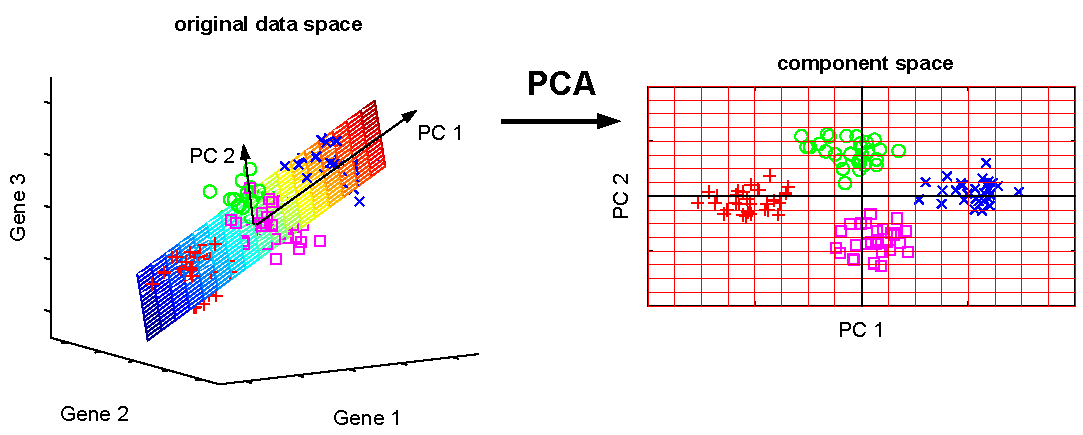
\includegraphics[width=0.47\textwidth]{figures/dim_reduct/fig_pca_illu3d}
  }% Store largest image in a box

  \begin{subfigure}[b]{0.48\textwidth}\centering
    \usebox{\largestimage}
    \vspace{0.01cm}
  \caption{PCA}
  \label{fig:dim_reduct:PCA:illustration}
  \end{subfigure}
  ~
  \begin{subfigure}[b]{\wd\largestimage}\centering
    \raisebox{\dimexpr.5\ht\largestimage-.5\height}{% Adjust vertical height of smaller image
      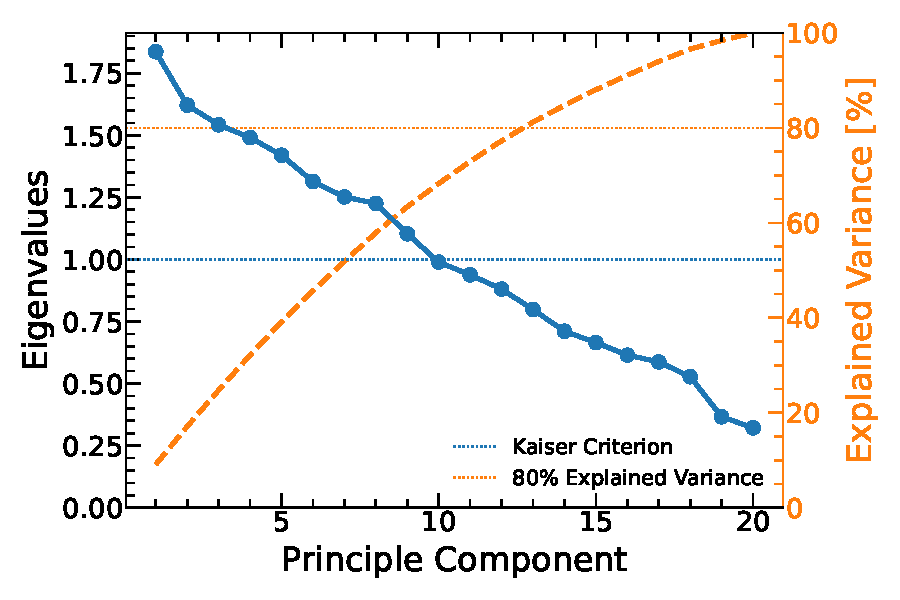
\includegraphics[width=\textwidth]{figures/dim_reduct/scree}}
  \caption{Scree Plot}
  \label{fig:dim_reduct:PCA:scree}
  \end{subfigure}
\caption{
On the left, an illustration of dimensionality reduction $m=3 \to k=2$ with PCA on genetics data \cite{Scholz2006}.
On the right, an example scree plot from a toy dataset.
Though there is no prominent elbow,
based on the Kaiser criterion (percent explainable variance)
we should consider reducing to $k=9$ ($k=13$) dimensions.
\label{fig:dim_reduct:PCA}
}
\end{figure}

%%%%%%%%%%%%%%%%%%%%%%%%%%%%%%%%%%%%%%%%%%%%%%%%%%%%%%%%
\subsection{Scree Plots}
\label{dim_reduct:PCA:scree}

When working with PCA we can use a
scree\footnote{Named after the similarly shaped geological feature, a rubble pile at the base of a cliff.} plot \cite{scree}
of the eigenvalues, such as \cref{fig:dim_reduct:PCA:scree},
to decide how many principle components to retain.
While this is always a somewhat subjective decision,
the Kaiser criterion \cite{kaiser_criterion} is one potential guideline,
keeping all principle components with $1 < \lambda_{i}$.
We can also look for an elbow in the plot,
or take the necessary principle components to reach
\si{80}{\percent} or $\si{90}{\percent} \leq \sum_{i=1}^{k} \lambda_{i} / \sum_{j=1}^{n} \lambda_{j}$ of the explainable variance.

%%%%%%%%%%%%%%%%%%%%%%%%%%%%%%%%%%%%%%%%%%%%%%%%%%%%%%%%
%%%%%%%%%%%%%%%%%%%%%%%%%%%%%%%%%%%%%%%%%%%%%%%%%%%%%%%%
\section{Singular Value Decomposition (SVD)}
\label{dim_reduct:SVD}
% TODO

%%%%%%%%%%%%%%%%%%%%%%%%%%%%%%%%%%%%%%%%%%%%%%%%%%%%%%%%
%%%%%%%%%%%%%%%%%%%%%%%%%%%%%%%%%%%%%%%%%%%%%%%%%%%%%%%%
\section{Linear Discriminant Analysis (LDA)}
\label{dim_reduct:LDA}
% TODO

% TODO include Gaussian Discriminant Analysis (GDA) and Quadratic Discriminant Analysis (QDA)

%%%%%%%%%%%%%%%%%%%%%%%%%%%%%%%%%%%%%%%%%%%%%%%%%%%%%%%%
%%%%%%%%%%%%%%%%%%%%%%%%%%%%%%%%%%%%%%%%%%%%%%%%%%%%%%%%
\section{Isomap}
\label{dim_reduct:isomap}
% TODO

%%%%%%%%%%%%%%%%%%%%%%%%%%%%%%%%%%%%%%%%%%%%%%%%%%%%%%%%
%%%%%%%%%%%%%%%%%%%%%%%%%%%%%%%%%%%%%%%%%%%%%%%%%%%%%%%%
\section{Factor Analysis and Confounding Variables}
\label{dim_reduct:factor_ana}
% TODO

%%%%%%%%%%%%%%%%%%%%%%%%%%%%%%%%%%%%%%%%%%%%%%%%%%%%%%%%
%%%%%%%%%%%%%%%%%%%%%%%%%%%%%%%%%%%%%%%%%%%%%%%%%%%%%%%%
\section{Mutual Information (MI)}
\label{dim_reduct:MI}
% TODO

%%%%%%%%%%%%%%%%%%%%%%%%%%%%%%%%%%%%%%%%%%%%%%%%%%%%%%%%
\subsection{Normalized Mutual Information (NMI)}
\label{dim_reduct:MI:normalized}
% TODO

%%%%%%%%%%%%%%%%%%%%%%%%%%%%%%%%%%%%%%%%%%%%%%%%%%%%%%%%
%%%%%%%%%%%%%%%%%%%%%%%%%%%%%%%%%%%%%%%%%%%%%%%%%%%%%%%%
\section{Term Frequency-Inverse Document Frequency (TF-IDF)}
\label{dim_reduct:tfidf}

Term frequency-inverse document frequency (TF-IDF) is a statistic
used in natural language processing (NLP) to quantify
the importance, or uniqueness, of a term $t$ in a document $d$
with respect to a wider set of documents $D$\footnote{Note that $d$ is not necessarily an element of $D$, we can compare novel $d$ to a reference corpus $D$.}.
As the name suggests, TF-IDF is the product of two components,
one representing the frequency of the term under consideration within the document of interest,
and the other the inverse of the frequency of the term in all documents of the broader corpus.
There are a handful of definitions available for each term, but we will only describe
one of the more standard forms in this section:

\begin{subequations}\label{eq:unsupervised:tfidf}
\begin{align}
\text{tf}\left(t,d\right) &= \frac{n_{t,d}}{\sum_{t' \in d} n_{t',d}}, \label{eq:unsupervised:tfidf:tf} \\
\text{idf}\left(t,D\right) &= \log\left(\frac{\abs{D}}{1 + \abs{\left\{d' \in D \, | \, t \in d'\right\}}}\right), \label{eq:unsupervised:tfidf:idf} \\
\text{tf-idf}\left(t,d\right) &= \text{tf}\left(t,d\right) \times \text{idf}\left(t,D\right). \label{eq:unsupervised:tfidf:tfidf}
\end{align}
\end{subequations}

\noindent Here $n_{t,d}$ is number of times $t$ appears in $d$,
$\abs{D}$ is the number of documents in $D$,
and $\abs{\left\{d \in D \, | \, t \in d\right\}}$ is the number of number of documents in $D$ which contain $t$.
We take the natural log in the $\text{idf}\left(t,D\right)$ component to better accommodate large corpora of documents,
and include the constant $1+$ term to avoid divide-by-zero issues.

%%%%%%%%%%%%%%%%%%%%%%%%%%%%%%%%%%%%%%%%%%%%%%%%%%%%%%%%
%%%%%%%%%%%%%%%%%%%%%%%%%%%%%%%%%%%%%%%%%%%%%%%%%%%%%%%%
\section{Prevalence Ratio}
\label{dim_reduct:prevalence_ratio}

The prevalence ratio (PR) is a similar concept to TF-IDF,
allowing us to identify important characteristics of a population of interest versus the wider population.
For example, we can use a PR to assess the association of hypertension with heart failure by comparing
the prevalence of hypertension in a cohort of heart failure patients
to the prevalence of hypertension in the general population,
or at least a representative sample\footnote{Defining an acceptable representative sample is often the hardest part of the analysis and may require stratification, \eg stratifying by age when investigating disease.} of it.

The prevalence of a characteristic $c$ in a population $P$ is $\abs{\{p' \in P \, | \, c \in p'\}} \, / \, \abs{p' \in P}$,
note the similarity to $\text{tf}\left(t,d\right)$ \cref{eq:unsupervised:tfidf:tf}.
The prevalence ratio is then

\begin{equation}\label{eq:unsupervised:PR}
\text{PR}\left(t,d\right) = \frac{ \abs{\{p' \in P \, | \, c \in p'\}} \, / \, \abs{p' \in P} }{ \abs{\{p' \in P_{0} \, | \, c \in p'\}} \, / \, \abs{p' \in P_{0}} },
\end{equation}

\noindent where $P$ is the population of interest and $P_{0}$ is the wider population.

Note that the PR is mathematically identical to the relative risk, or hazard ratio (HR) discussed in \cref{chap:survival}.
There is a similar discussion in the literature \cite{pmid27460748,10.3389/fvets.2017.00193}
on prevalence ratios versus odds ratios as is described in \cref{survival:additional:odds}.

% See also: https://sph.unc.edu/wp-content/uploads/sites/112/2015/07/nciph_ERIC8.pdf

%%%%%%%%%%%%%%%%%%%%%%%%%%%%%%%%%%%%%%%%%%%%%%%%%%%%%%%%
%%%%%%%%%%%%%%%%%%%%%%%%%%%%%%%%%%%%%%%%%%%%%%%%%%%%%%%%
\section{\texorpdfstring{$t$}{t}-Distributed Stochastic Neighbor Embedding (\texorpdfstring{$t$}{t}-SNE)}
\label{dim_reduct:tSNE}
% TODO
% TODO \tSNE
}
%%%%%%%%%%%%%%%%%%%%%%%%%%%%%%%%%%%%%%%%%%%%%%%%%%%%%%%%
%%%%%%%%%%%%%%%%%%%%%%%%%%%%%%%%%%%%%%%%%%%%%%%%%%%%%%%%
%%%%%%%%%%%%%%%%%%%%%%%%%%%%%%%%%%%%%%%%%%%%%%%%%%%%%%%%
\chapter{Optimization}
\label{chap:opt}
% TODO
% TODO many types of optimizers, two main classes of gradient and non-gradient methods.
% TODO A greedy optimizer finds the local optimum at each iteration, which may or may not converge to a global optimum.

%%%%%%%%%%%%%%%%%%%%%%%%%%%%%%%%%%%%%%%%%%%%%%%%%%%%%%%%
%%%%%%%%%%%%%%%%%%%%%%%%%%%%%%%%%%%%%%%%%%%%%%%%%%%%%%%%
\section{Maximum Likelihood Estimation (MLE)}
\label{opt:MLE}

Maximum likelihood estimation (MLE) is a method
of choosing the optimal parameters of a probability distribution
to match some set of observed data.
As the name suggests, MLE works by maximizing the likelihood of observing the given data.
Note that the terms likelihood and probability are closely related, but different, in this context.
Here probability refers to the probability of observing $x$ given parameters $\vb*{\beta}$, $P\left(x \mid \vb*{\beta}\right)$,
while likelihood refers to the likelihood of the distribution having parameters $\vb*{\beta}$ given an observation $x$, $L\left(\vb*{\beta} \mid x\right)$.
$L$ and $P$ are both equal to relevant probability distribution,
such as \cref{eq:stats:gaus:P} for the Gaussian distribution,
but which variables are independent and dependent changes.

As we wish to maximize the likelihood with respect to $\vb*{\beta}$,
we will be taking partial derivatives and finding where they equal zero, $\partial_{\vb*{\beta}} L = 0$.
In practice, likelihood functions are complicated\footnote{The value of $L$
is often close to $0$, making lack of precision an issue when doing computations.
$\log\left(L\right)$ is larger and also helps address this problem.} and
it is easier to maximize the log-likelihood $\log\left(L\right)$,
which has the same maximum as the original likelihood $L$,
but removes exponents and turns multiplication in to addition.
Generally there are $m$ points $\vb{x}_{i}$, each with $n$ dimensions, in a given dataset,
thus we are solving \cref{eq:MLE} for $\vb*{\beta} = \hat{\vb*{\beta}}_{\text{MLE}}$:

\begin{subequations}\label{eq:MLE}
\begin{align}
0 &= \partial_{\vb*{\beta}} \, L\left(\vb*{\beta} \mid \vb{x}\right) \label{eq:MLE:L} \\
\implies 0 &= \partial_{\vb*{\beta}} \log\left(L\left(\vb*{\beta} \mid \mathbf{X}\right)\right) = \partial_{\vb*{\beta}} \, \log\left(\prod_{i=1}^{m} \, P\left(\vb{x}_{i} \mid \vb*{\beta}\right)\right) \label{eq:MLE:log_L} \\
&= \sum_{i=1}^{m} \, \partial_{\vb*{\beta}} \log\left(P\left(\vb{x}_{i} \mid \vb*{\beta}\right)\right) \label{eq:MLE:log_L_sum}
\end{align}
\end{subequations}

In practice, it is unlikely that a closed form solution for $\hat{\vb*{\beta}}_{\text{MLE}}$ can be found
and numerical optimizers, such as gradient descent, are used instead.
Under certain conditions it can be shown that as $n \to \infty$ the MLE converges to $\hat{\vb*{\beta}}$,
\ie in the limit $n \to \infty$ no consistent estimator
has a lower MSE\footnote{More formally, the MLE achieves the Cram\'er--Rao lower bound.}.
Lastly, while the MLE is usually a biased estimator, see \cref{stats:bias},
the bias is also reduced as $n \to \infty$.

%%%%%%%%%%%%%%%%%%%%%%%%%%%%%%%%%%%%%%%%%%%%%%%%%%%%%%%%
\subsection{Exponential Distribution Example}
\label{opt:MLE:exp_ex}

We can use MLE to find the optimal $\hat{\lambda}_{\text{MLE}}$ of
the exponential distribution \cref{eq:stats:exp:P}
given a dataset of $m$ points, $x_{i}$, in 1 dimension:

\begin{subequations}\label{eq:MLE:exp_ex}
\begin{align}
0 &= \sum_{i=1}^{m} \partial_{\lambda} \log\left(P\left(x_{i} \mid \lambda\right)\right) = \sum_{i=1}^{m} \partial_{\lambda} \log\left(\lambda e^{-\lambda x_{i}}\right), \label{eq:MLE:exp_ex:log_L_sum} \\
&= \sum_{i=1}^{m}\partial_{\lambda} \left( \log\left(\lambda\right) -\lambda x_{i}\right) = \sum_{i=1}^{m} \frac{1}{\lambda} - x_{i} = \frac{m}{\lambda} - \sum_{i=1}^{m} x_{i}, \label{eq:MLE:exp_ex:solve} \\
\implies \hat{\lambda}_{\text{MLE}} &= \frac{m}{\sum_{i=1}^{m} x_{i}} = \frac{1}{\expval{x}}. \label{eq:MLE:exp_ex:lambda}
\end{align}
\end{subequations}

For another example of MLE see logistic regression \cref{eq:logistic:L_Pr}.

%%%%%%%%%%%%%%%%%%%%%%%%%%%%%%%%%%%%%%%%%%%%%%%%%%%%%%%%
%%%%%%%%%%%%%%%%%%%%%%%%%%%%%%%%%%%%%%%%%%%%%%%%%%%%%%%%
\section{Maximum A Posteriori (MAP)}
\label{opt:MAP}
% TODO In maximum \aposteriori (MAP) estimation
% TODO MLE is a special case of MAP with a uniform prior

%%%%%%%%%%%%%%%%%%%%%%%%%%%%%%%%%%%%%%%%%%%%%%%%%%%%%%%%
%%%%%%%%%%%%%%%%%%%%%%%%%%%%%%%%%%%%%%%%%%%%%%%%%%%%%%%%
\section{Gradient Descent}
\label{opt:grad_descent}
% TODO

%%%%%%%%%%%%%%%%%%%%%%%%%%%%%%%%%%%%%%%%%%%%%%%%%%%%%%%%
\subsection{Stochastic Gradient Descent (SGD)}
\label{opt:grad_descent:stochastic}
% TODO

%%%%%%%%%%%%%%%%%%%%%%%%%%%%%%%%%%%%%%%%%%%%%%%%%%%%%%%%
%%%%%%%%%%%%%%%%%%%%%%%%%%%%%%%%%%%%%%%%%%%%%%%%%%%%%%%%
\section{Lagrange Multipliers}
\label{opt:lagrange_mult}
% TODO

%%%%%%%%%%%%%%%%%%%%%%%%%%%%%%%%%%%%%%%%%%%%%%%%%%%%%%%%
%%%%%%%%%%%%%%%%%%%%%%%%%%%%%%%%%%%%%%%%%%%%%%%%%%%%%%%%
\section{Newton's Method}
\label{opt:newton}
% TODO

%%%%%%%%%%%%%%%%%%%%%%%%%%%%%%%%%%%%%%%%%%%%%%%%%%%%%%%%
%%%%%%%%%%%%%%%%%%%%%%%%%%%%%%%%%%%%%%%%%%%%%%%%%%%%%%%%
\section{Exploration-Exploitation Tradeoff}
\label{opt:EE_tradeoff}
% TODO

%%%%%%%%%%%%%%%%%%%%%%%%%%%%%%%%%%%%%%%%%%%%%%%%%%%%%%%%
%%%%%%%%%%%%%%%%%%%%%%%%%%%%%%%%%%%%%%%%%%%%%%%%%%%%%%%%
\section{Bayesian Bandits}
\label{opt:BB}
% TODO

%%%%%%%%%%%%%%%%%%%%%%%%%%%%%%%%%%%%%%%%%%%%%%%%%%%%%%%%
%%%%%%%%%%%%%%%%%%%%%%%%%%%%%%%%%%%%%%%%%%%%%%%%%%%%%%%%
\section{Evolutionary \& Genetic Algorithms}
\label{opt:evo}
% TODO

%%%%%%%%%%%%%%%%%%%%%%%%%%%%%%%%%%%%%%%%%%%%%%%%%%%%%%%%
%%%%%%%%%%%%%%%%%%%%%%%%%%%%%%%%%%%%%%%%%%%%%%%%%%%%%%%%
\section{Bayesian Optimization}
\label{opt:BO}

Frequently we are fortunate enough to have a fairly explicit form of
the objective function $S\left(\vb*{\beta}\right)$ to be optimized in order to solve a problem.
However, when $S\left(\vb*{\beta}\right)$ is not well-known,
is expensive to compute\footnote{The performance of a machine learning model as a function of its hyperparameters is a classic example of this.
In that case, evaluating $S$ amounts to training the model with a particular set of hyperparameters $\vb*{\beta}$,
then determining it's performance on a metric such as ROC AUC.}, or is non-differentiable,
the usual gradient based approaches, such as SGD and Newton's method, break down.
In these cases ``black box''\footnote{Black box as in
we do not have a closed-form expression for $S$, or know $\grad S$.} methods\footnote{Other examples of black box optimizers include
Tree-Structured Parzen Estimators (TPE),
genetic algorithms,
and some additional tree based methods described in \cite{Hutter2011,Hutter2014}.
A TPE is a close relative of Bayesian optimization, making use of the opposite side of Bayes' theorem by
estimating $P\left(\vb*{\beta} \mid S\right)$ and $P\left(S\right)$ rather than $P\left(S \mid \vb*{\beta}\right)$.
TPEs can accommodate categorical $\beta_{i}$ in a hierarchical manner,
however they can not model interactions between the $\beta_{i}$ \cite{bissuel_2019,NIPS2011_4443}.},
such as Bayesian optimization, may be used instead.

In Bayesian optimization\footnote{Generalized
formally as Sequential Model-Based Optimization (SMBO) \cite{NIPS2011_4443}.} \cite{Brochu2010,1301.1942,Borisyak,NIPS2011_4443},
$S$ is approximated by a well-known surrogate function\footnote{Also known as a response surface.}.
The surrogate typically is a Gaussian process (GP),
but can be any well-behaved regressor such as
a Random Forest or Boosted Decision Tree (BDT).
GPs \cref{eq:GP} are
extensions of Gaussian distributions which return a Gaussian at any point along their domain.
They are parameterized by a mean function\footnote{For convenience,
the prior $m\left(\vb{x}\right)$ is usually assumed to be zero, $m\left(\vb{x}\right)=0$.}, $m\left(\vb{x}\right)$,
and covariance function, $k\left(\vb{x}_{i}, \vb{x}_{j}\right)$,
\ie kernel\footnote{The kernel of the GP is a hyperparameter to be chosen in advance.
Standard kernel choices include
the radial basis function kernel $k\left(\vb{x}_{i}, \vb{x}_{j}\right) = \exp\left(-\frac{1}{2\sigma^{2}}\norm{\vb{x}_{i}-\vb{x}{j}}^{2}\right)$,
Mat\'{e}rn kernel,
and white noise kernel $k\left(\vb{x}_{i}, \vb{x}_{j}\right) \propto \delta_{ij}$.},
instead of a constant mean $\mu$ and variance $\sigma^{2}$.
An illustration of a GP is provided in \cref{fig:GP_ex}.

\begin{equation}\label{eq:GP}
f\left(\vb{x}\right) \sim \mathcal{GP}\left(m\left(\vb{x}\right), k\left(\vb{x}_{i}, \vb{x}_{j}\right)\right).
\end{equation}

\begin{figure}[H] % TODo might want to eventually remove
\centering
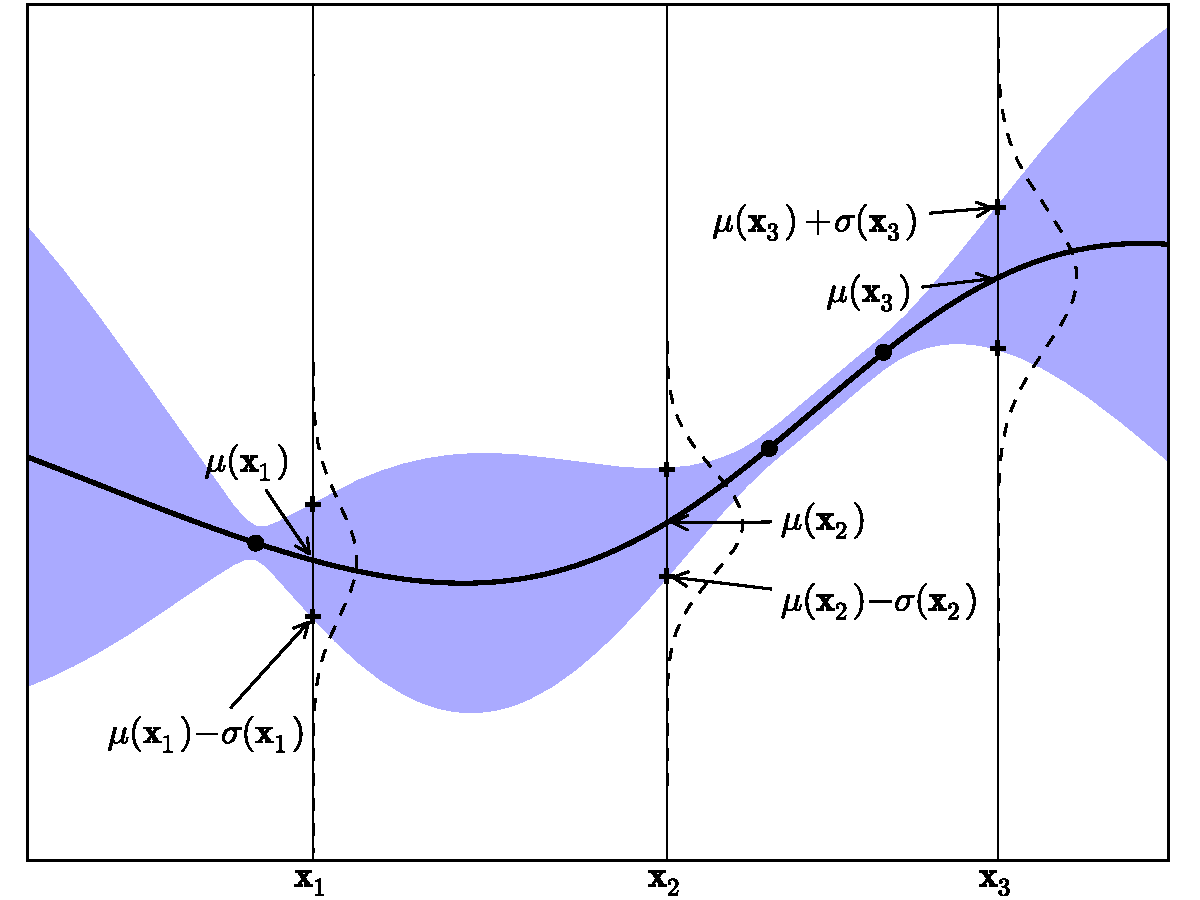
\includegraphics[width=0.85\textwidth]{figures/ml/gp}
\caption{
Illustration of a Gaussian process (GP) in 1D \cite{Brochu2010}.
Note that at any point $\vb{x}_{1}$, $\vb{x}_{2}$, $\vb{x}_{3}$ the GP
returns a Gaussian distribution characterizing the estimated mean and uncertainty on the
unknown true function, \ie the objective function $S\left(\vb*{\beta}\right)$ in the case of Bayesian optimization.
}
\label{fig:GP_ex}
\end{figure}

The surrogate function is initially fit to
a random sample of $\vb*{\beta}$, $S\left(\vb*{\beta}\right)$ points.
From this prior, Bayesian optimization
operates by iteratively sampling $S\left(\vb*{\beta}\right)$ and updating
the posterior surrogate function as each new piece of information is gained.
An acquisition function, $u\left(\cdot\right)$, directs the sampling,
estimating where $S\left(\vb*{\beta}\right)$ may be large
due to a high predicted value, large uncertainty, or some combination of the two.
The exploration-exploitation tradeoff inherent in $u\left(\cdot\right)$
can be tuned in various ways, see Section 2.3 of \cite{Brochu2010} for a full description\footnote{Common types of acquisition function include the
Expected Improvement (EI);
$\text{EI}\left(\vb*{\beta}\right) = \expvalE{\max\left(0,\,S\big(\vb*{\beta}\big) - S\big(\hat{\vb*{\beta}}\big)\right)}$
where $S\big(\hat{\vb*{\beta}}\big)$ is the current optimal value of $S$,
Upper Confidence Bound (UCB);
$\text{UCB}\left(\vb*{\beta}\right) = E_{\text{GP}} \left(\vb*{\beta}\right) + \kappa\,\text{var}_{\text{GP}} \left(\vb*{\beta}\right)$ where the mean and variance are of the GP and $\kappa$ sets the exploration-exploitation tradeoff,
and Maximum Probability of Improvement (MPI).}.
The iterative nature of Bayesian optimization is illustrated in \cref{fig:BO_ex}.
An accessible implementation of Bayesian optimization is available in \skopt \cite{scikit-optimize,Borisyak}.

\begin{figure}[H] % TODo might want to eventually remove
\centering
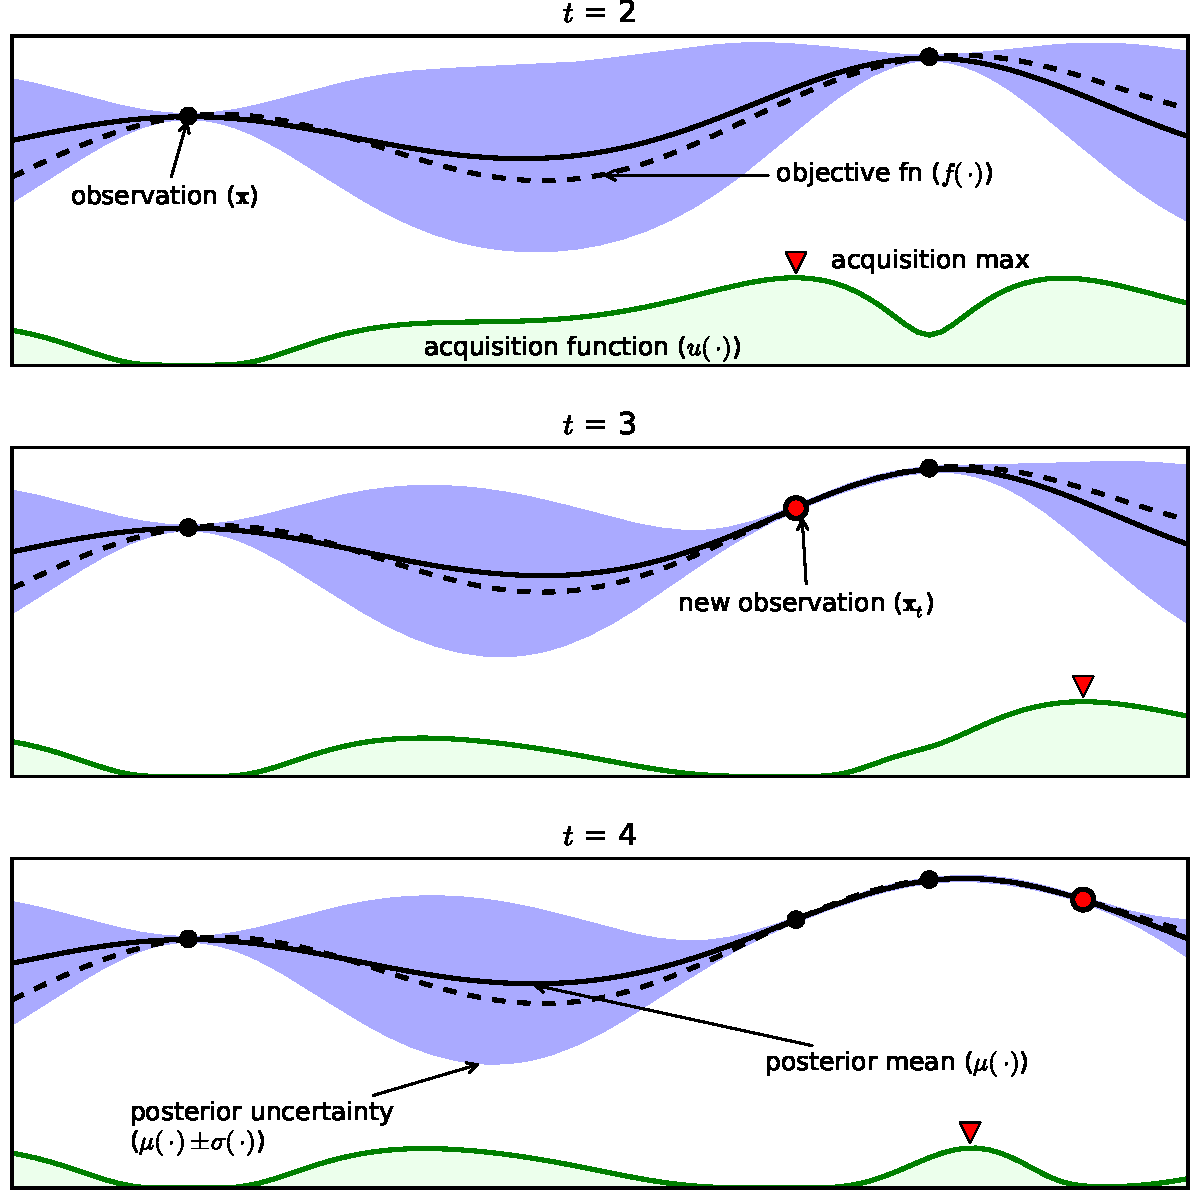
\includegraphics[width=0.85\textwidth]{figures/ml/toyGPtext3}
\caption{
Illustration of Bayesian optimization over three iterations in a toy 1D maximization problem \cite{Brochu2010}.
Note that the maximum of the acquisition function $u\left(\cdot\right)$
locates where $S\left(\vb*{\beta}\right)$ should be sampled next.
The GP estimated posterior distribution of $S\left(\vb*{\beta}\right)$
and $u\left(\cdot\right)$ are then updated.
This iterative process is repeated until the estimated maximum is satisfactory.
}
\label{fig:BO_ex}
\end{figure}

%%%%%%%%%%%%%%%%%%%%%%%%%%%%%%%%%%%%%%%%%%%%%%%%%%%%%%%%
%%%%%%%%%%%%%%%%%%%%%%%%%%%%%%%%%%%%%%%%%%%%%%%%%%%%%%%%
\section{Minimum Mean Square Error (MMSE) Estimator}
\label{opt:BO:MMSE}
% TODO
}
%%%%%%%%%%%%%%%%%%%%%%%%%%%%%%%%%%%%%%%%%%%%%%%%%%%%%%%%
%%%%%%%%%%%%%%%%%%%%%%%%%%%%%%%%%%%%%%%%%%%%%%%%%%%%%%%%
%%%%%%%%%%%%%%%%%%%%%%%%%%%%%%%%%%%%%%%%%%%%%%%%%%%%%%%%
\chapter{Classification}
\label{chap:class}

%%%%%%%%%%%%%%%%%%%%%%%%%%%%%%%%%%%%%%%%%%%%%%%%%%%%%%%%
%%%%%%%%%%%%%%%%%%%%%%%%%%%%%%%%%%%%%%%%%%%%%%%%%%%%%%%%
\section{Logistic Regression}
\label{class:logistic}

Logistic regression is a simple method to create a classifier,
typically on two classes $y = 0,1$, though multinomial extensions exist.
Its name comes from the use of the logit, or log-odds, function

\begin{equation}\label{eq:logistic:logic}
l = \text{logit}\left(p\right) = \log\left(\frac{p}{1-p}\right)
\end{equation}

\noindent on the probability $p$ of class $1$.
$l$ is estimated linearly from $n$ input features $x_{j}$ with $n+1$ parameters $\beta_{j}$ as:

\begin{equation}\label{eq:logistic:logicBeta}
l = \beta_{0} + \sum_{j=1}^{n} \, \beta_{j}\,x_{j}\,.
\end{equation}

\noindent The probability $p$ is then

\begin{equation}\label{eq:logistic:p}
p = \frac{e^l}{e^l + 1} = \frac{1}{1+e^{-l}} = \text{logit}^{-1}\left(l\right)
\end{equation}

\noindent which can be turned into a predicted class through the choice of a suitable decision threshold.

The model parameters $\vb*{\beta}$ are chosen by maximizing
the log of the likelihood $L$ \cref{eq:logistic:L} over $m$ known example points $\vb{x}_{i}, y_{i}$.
Note that $P\left(y \mid x\right)$ \cref{eq:logistic:Pr} is simply the Bernoulli distribution.
In practice the log-likelihood $\log\left(L\right)$ is maximized via gradient descent.
An example of logistic regression can be found in \cref{fig:logistic_regression_ex}.

\begin{subequations} \label{eq:logistic:L_Pr}
\begin{align}
L\left(\vb*{\beta} \mid \vb{x}\right) &= \prod_{i=1}^{m} \, P\left(y_{i} \mid \vb{x}_{i};\,\vb*{\beta}\right) \label{eq:logistic:L} \\
P\left(y \mid \vb{x}\right) &= p^y\left(1-p\right)^{1-y}, \quad y \in \{0, 1\} \label{eq:logistic:Pr}
\end{align}
\end{subequations}

\begin{figure}
\centering
% 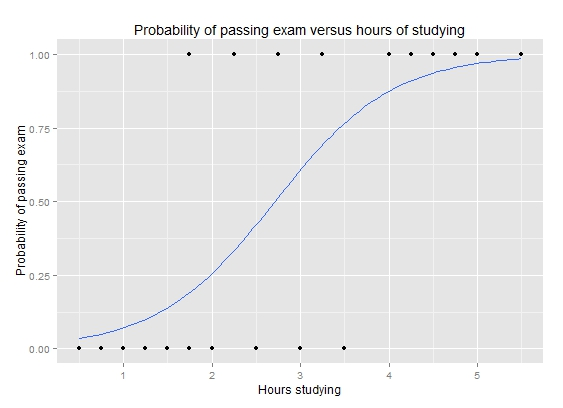
\includegraphics[width=0.8\textwidth]{figures/regression/Exam_pass_logistic_curve.jpeg}
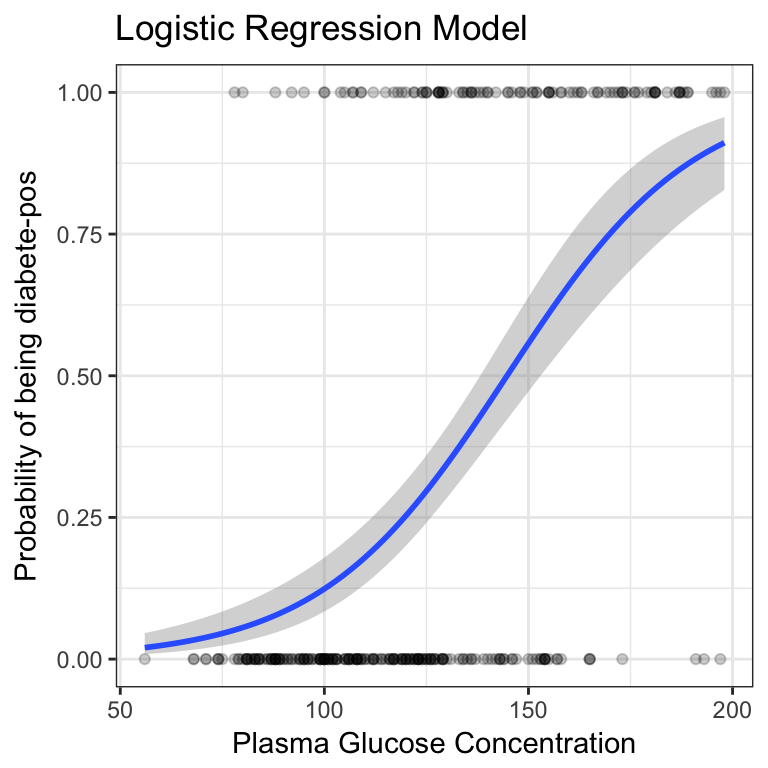
\includegraphics[width=0.7\textwidth]{figures/regression/logistic-regression-probabilities-curve.png}
\caption{
% Example logistic regression curve on one input feature, by \href{https://en.wikipedia.org/wiki/File:Exam_pass_logistic_curve.jpeg}{Michaelg2015}.
Example logistic regression curve on one input feature, by \href{http://www.sthda.com/english/articles/36-classification-methods-essentials/151-logistic-regression-essentials-in-r/}{Kassambara}.
}
\label{fig:logistic_regression_ex}
\end{figure}

%%%%%%%%%%%%%%%%%%%%%%%%%%%%%%%%%%%%%%%%%%%%%%%%%%%%%%%%
\subsection{Assumptions}
\label{class:logistic:assumptions}
% TODO

% TODO any more assumptions?
Some assumptions of the logistic regression approach are:
\begin{enumerate}[noitemsep]
  \item $y$ is either present or absent (dichotomous).
  \item There are minimal correlations between the $x_{j}$ features (no multicollinearity).
  \item There are no major outliers in the data.
\end{enumerate}

% TODO pseudo R2, Wald statistic
% TODO regularized versions?

%%%%%%%%%%%%%%%%%%%%%%%%%%%%%%%%%%%%%%%%%%%%%%%%%%%%%%%%
\subsection{Example}
\label{class:logistic:example}
% TODO

%%%%%%%%%%%%%%%%%%%%%%%%%%%%%%%%%%%%%%%%%%%%%%%%%%%%%%%%
%%%%%%%%%%%%%%%%%%%%%%%%%%%%%%%%%%%%%%%%%%%%%%%%%%%%%%%%
\section{N{a\"i}ve Bayes Classification}
\label{class:Bayes}
% TODO
% TODO maximum a posteriori (italics) probability (MAP) estimator

%%%%%%%%%%%%%%%%%%%%%%%%%%%%%%%%%%%%%%%%%%%%%%%%%%%%%%%%
\subsection{Gaussian N{a\"i}ve Bayes Classification (GNB)}
\label{class:Bayes:GNB}
% TODO

%%%%%%%%%%%%%%%%%%%%%%%%%%%%%%%%%%%%%%%%%%%%%%%%%%%%%%%%
%%%%%%%%%%%%%%%%%%%%%%%%%%%%%%%%%%%%%%%%%%%%%%%%%%%%%%%%
\section{Support Vector Machines (SVM)}
\label{class:SVM}

Basic support vector machines (SVM) work by finding a hyperplane in the $n$-dimensional
feature space of the training data which best separate the different classes.
This is done by maximizing the margin, $2/\norm{\vb{w}}$,
around the hyperplane defined by $\innerproduct{\vb{w}}{\vb{x}} - b = 0$,
where $\innerproduct{\vb{a}}{\vb{b}}$ is the inner product.
For the separable case, as shown in \cref{fig:svm_sep}, this
can be done by minimizing $\norm{\vb{w}}$, with the hard-margin condition that
$y_{i} \left(\innerproduct{\vb{w}}{\vb{x}_{i}} - b\right)$ for all $1 \leq i \leq m$.

However, in reality the data are frequently inseparable and we must switch
to a soft-margin objective function \cref{eq:svm:soft_margin_obj}.
A hinge loss function is included to penalize points on the ``wrong'' side of the margin
proportionally to their distance from the margin.
Here the $\lambda$ hyperparameter sets the tradeoff between
margin size and ensuring points land on their correct sides.

\begin{equation} \label{eq:svm:soft_margin_obj}
S\left(\vb{w}, b\right) =
\lambda\, \norm{\vb{w}}^{2}
+ \frac{1}{m} \sum_{i=1}^{m} \,
\max{\big(0,\, 1 - y_{i} \left(\innerproduct{\vb{w}}{\vb{x}_{i}} - b\right)\big)}.
\end{equation}

\begin{figure}[H]
\centering
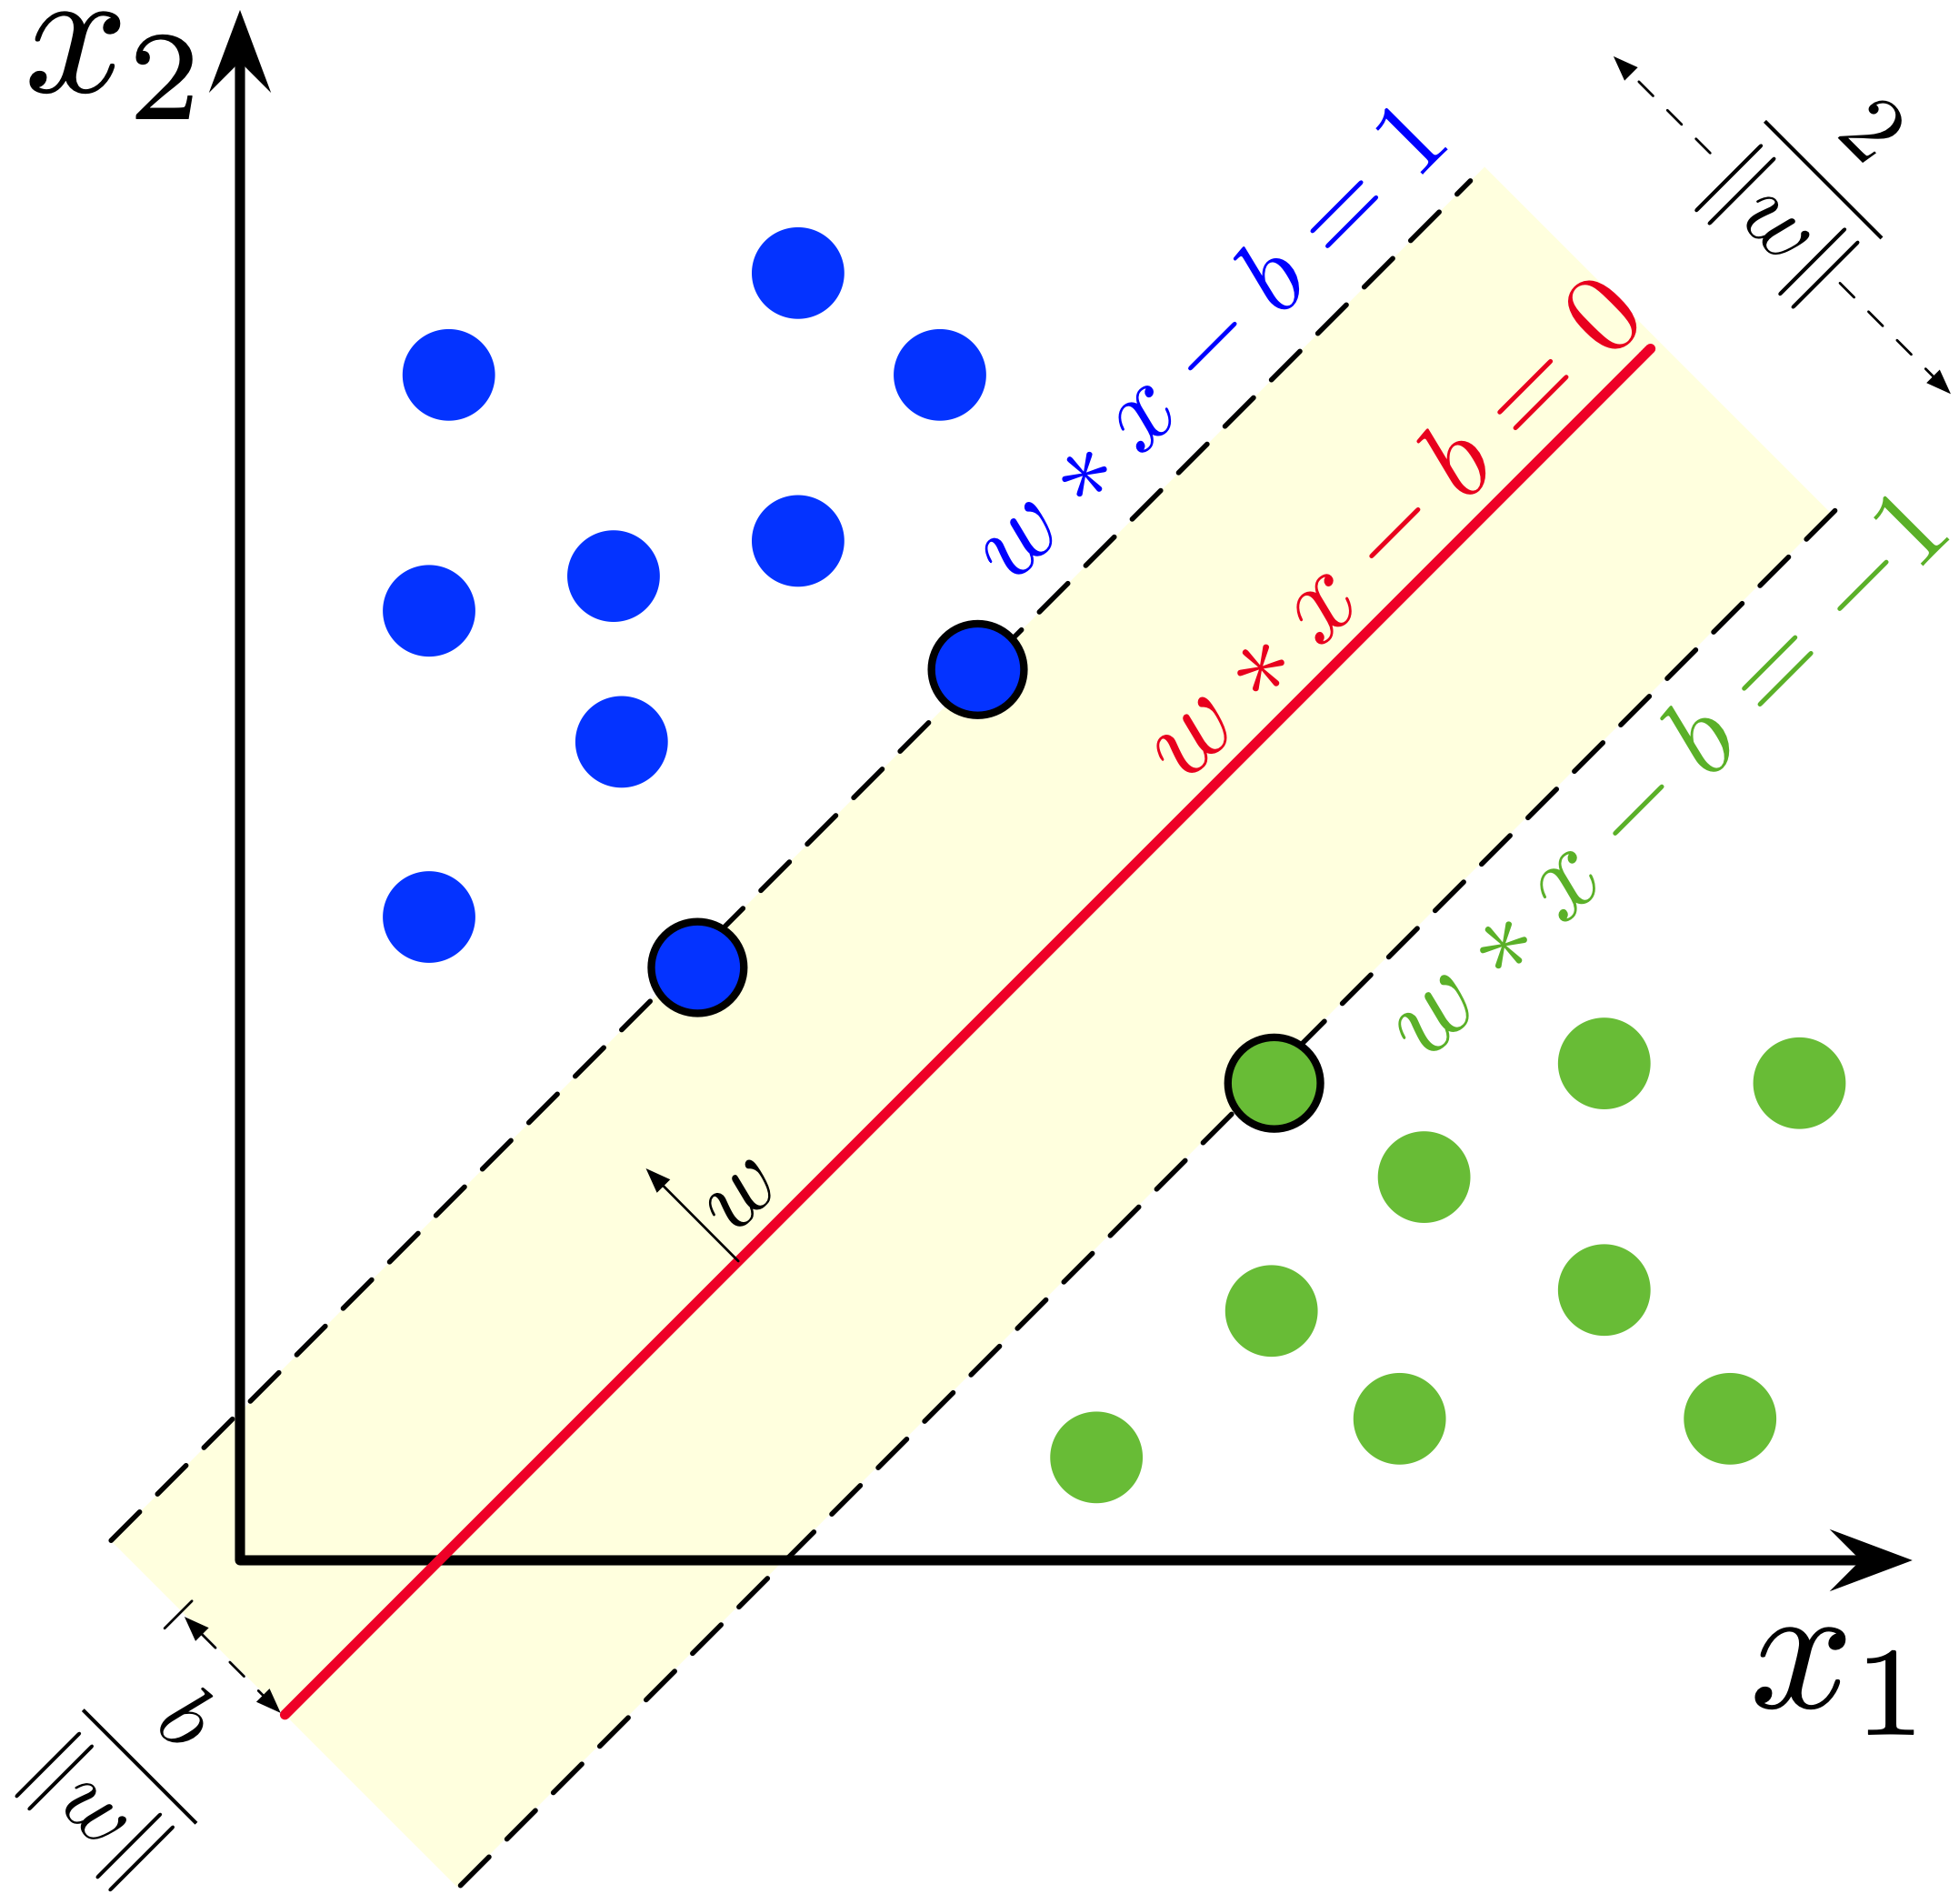
\includegraphics[width=0.42\textwidth]{figures/ml/svm_margin.png}
\vspace{0.2cm}
\caption{
Illustration of the SVM method in the separable case,
by \href{https://en.wikipedia.org/wiki/File:SVM_margin.png}{Larhmam}.
The trained hyperplane in red separates the two classes by the largest margin.
The data points on the margin boundary with black boarders
are known as support vectors, since out of all the data
they are the points really fixing the hyperplane and margin.
}
\label{fig:svm_sep}
\end{figure}

To gain better performance still, we can recast the problem in
a new higher dimensional space where the classes may be easier to separate with a hyperplane.
Fortunately, we don't even need to fully specify the new space,
just a non-linear kernel function\footnote{Common kernel choices include
polynomials of the inner product,
the Gaussian radial basis function,
and the hyperbolic tangent.} $k\left(\vb{a},\vb{b}\right)$
in place of the standard inner product. This is known as the kernel trick.
The classification boundary in the original feature space can then become non-linear,
as can be seen in \cref{fig:svm_kernel_trick}.

\vspace{-0.3cm}% TODo hard coded to fit on one page

\begin{figure}[H]
\centering
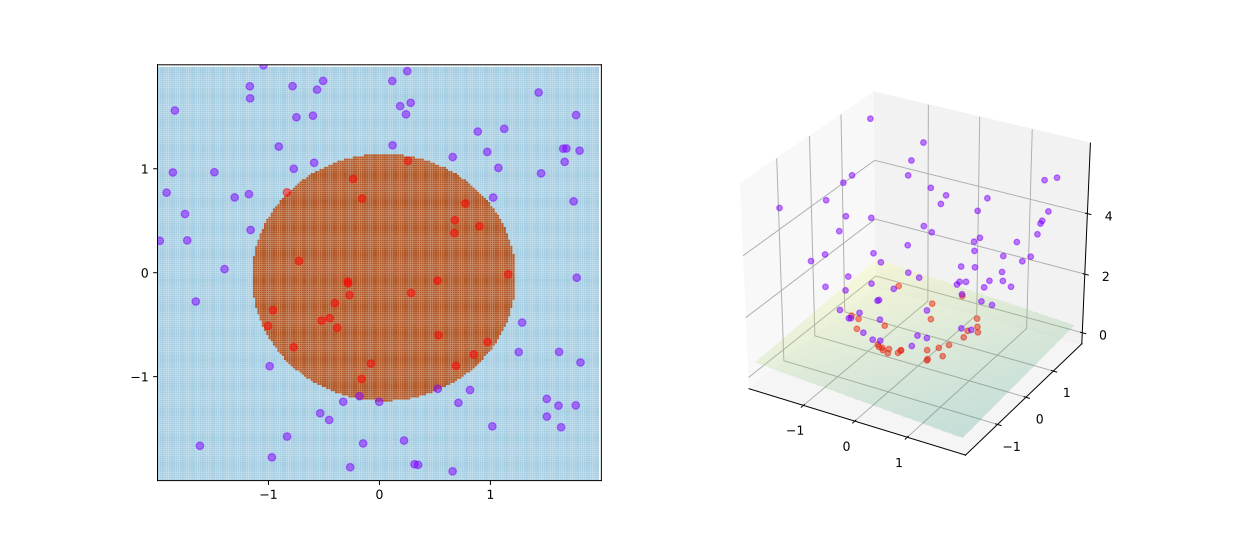
\includegraphics[width=0.8\textwidth,trim={4.0cm 0.8cm 4.0cm 1.4cm},clip]{figures/ml/kernel_trick_example.png}% trim={<left> <lower> <right> <upper>}
\caption{
Graphical example of the kernel trick, by \href{https://en.wikipedia.org/wiki/File:Kernel_trick_idea.svg}{Shiyu Ji}.
Here the kernel $k\left(\vb{a},\vb{b}\right) = \innerproduct{\vb{a}}{\vb{b}} + \norm{\vb{a}}^{2} \norm{\vb{b}}^{2}$
transforms the red and purple classes, linearly inseparable in $n=2$ dimensions on the left,
to a separable $3$-dimensional space on the right.
}
\label{fig:svm_kernel_trick}
\end{figure}

In practice minimizing $S\left(\vb{w}, b\right)$ can be
performed more readily by instead solving the Lagrangian dual problem,
which is computationally efficient to solve with quadratic programming algorithms.
Other modern techniques developed to tackle large and sparse data include
sub-gradient methods and coordinate descent\footnote{Sub-gradient methods work better for large $m$,
coordinate descent for large $n$.}.
However, compared to other classifiers SVM training times
tend to slow significantly for large datasets,
in \sklearn\footnote{See the
\href{https://scikit-learn.org/stable/modules/generated/sklearn.svm.SVC.html}{documentation}
for \texttt{sklearn.svm.SVC}.
\texttt{LinearSVC} may be faster.
The best performance I've seen quoted is $\order{n m \log{\left(m\right)}}$.} by
at least $\order{m^{2}}$, limiting $m \sim \num{e4}$.

%\begin{figure}[H]
%  \centering
%  \begin{subfigure}[b]{0.48\textwidth}\centering
%      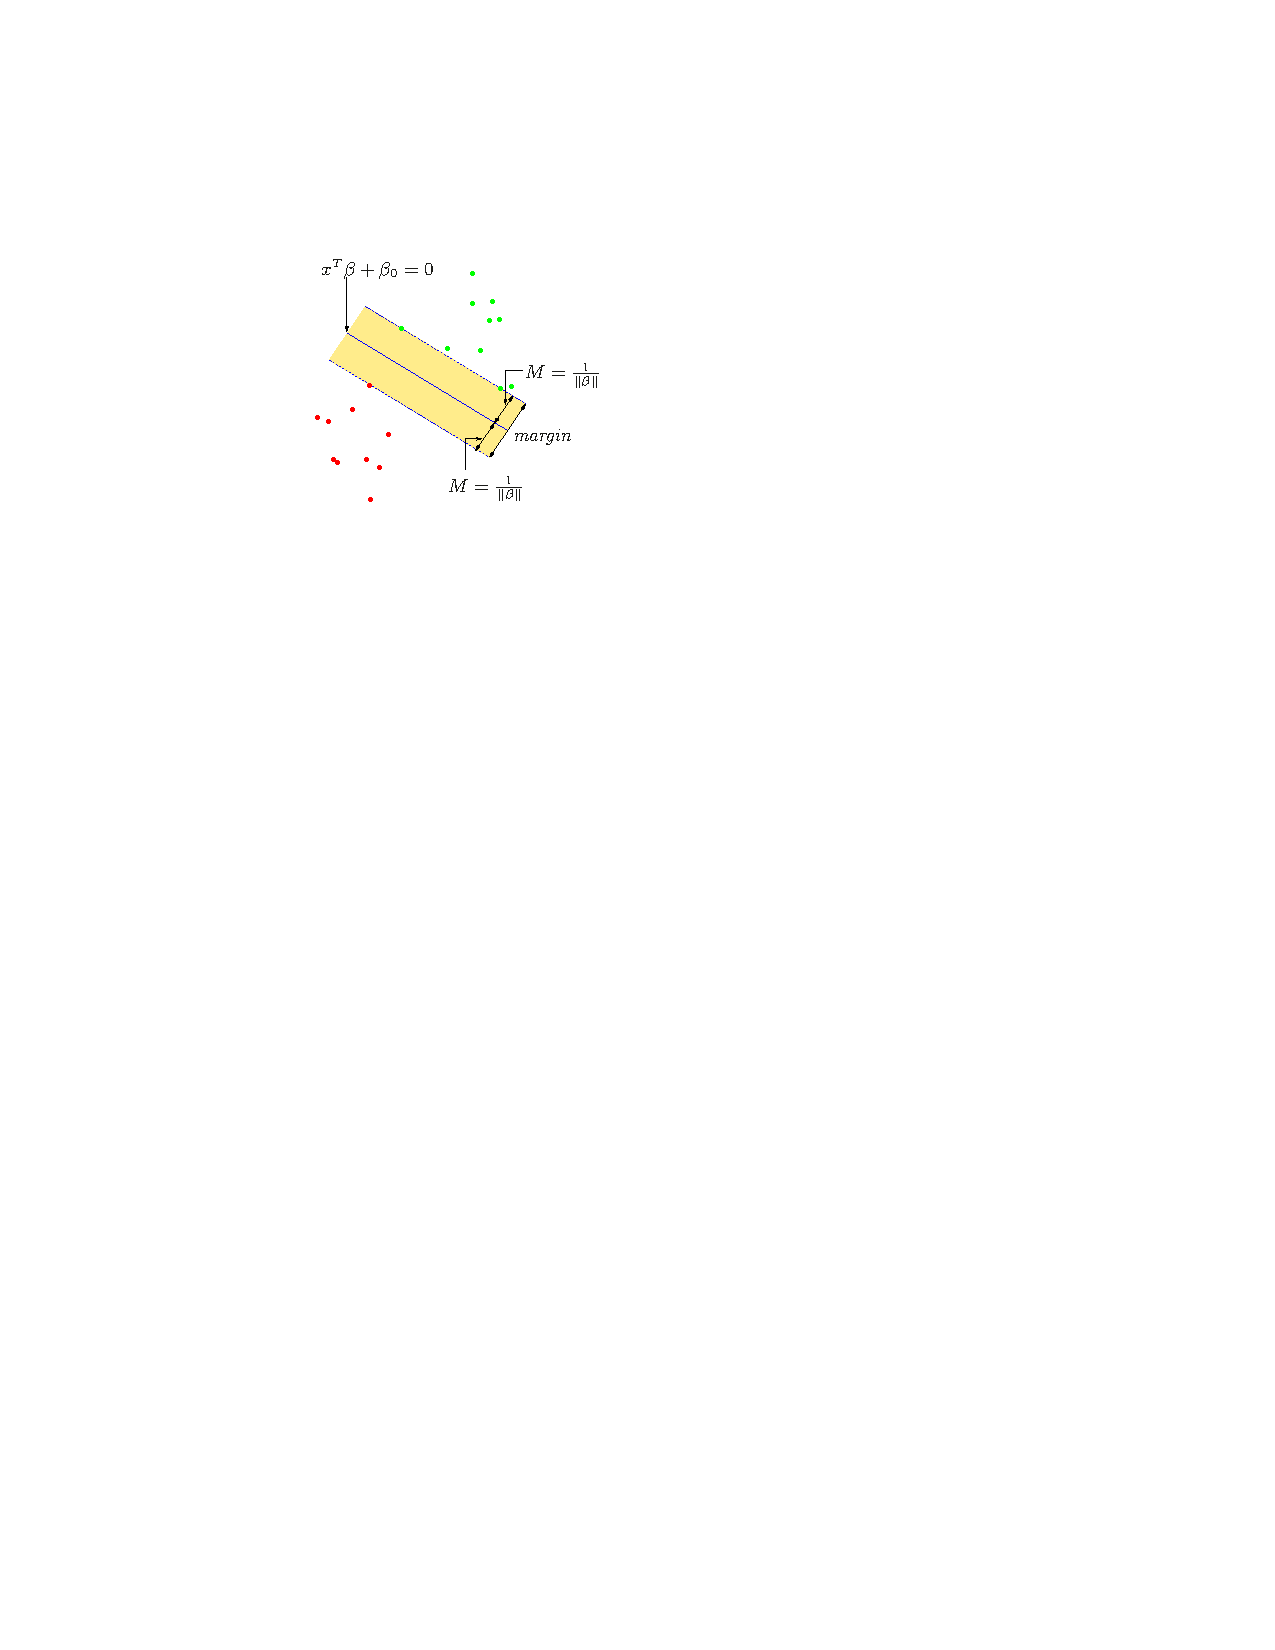
\includegraphics[width=\textwidth]{figures/ml/svm_separable}
%  \caption{Separable}
%  \label{fig:svm:separable}
%  \end{subfigure}
%  ~
%  \begin{subfigure}[b]{0.48\textwidth}\centering
%      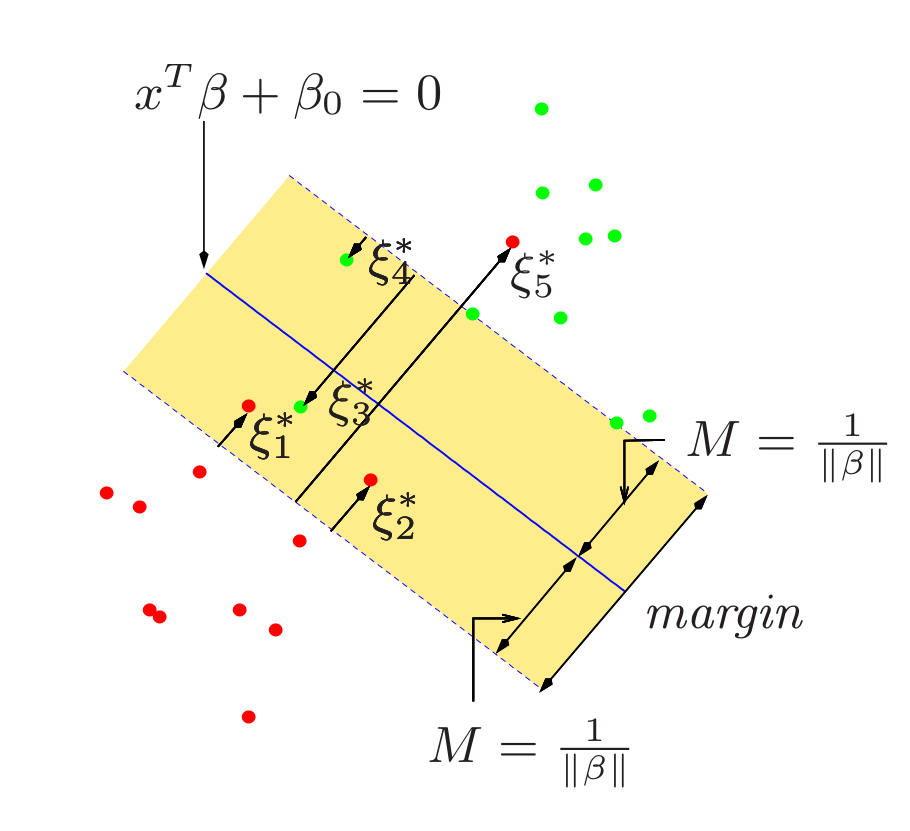
\includegraphics[width=\textwidth]{figures/ml/svm_nonseparable}
%  \caption{Nonseparable}
%  \label{fig:svm:nonseparable}
%  \end{subfigure}
%\caption{
%Illustrations of SVMs in the separable and nonseparable case \cite{HastieTF09}.
%\label{fig:svm}
%}
%\end{figure}

%%%%%%%%%%%%%%%%%%%%%%%%%%%%%%%%%%%%%%%%%%%%%%%%%%%%%%%%
%%%%%%%%%%%%%%%%%%%%%%%%%%%%%%%%%%%%%%%%%%%%%%%%%%%%%%%%
\section{Decision Trees, \texorpdfstring{\ie}{ie} Classification and Regression Trees (CART)}
\label{class:CART}

A basic classifier can be created from a tree of selections on $\mb{X}$ designed to
separate the classes at each branch.
Such a model is known as a classification and regression tree (CART) \cite{Breiman:2253780},
and a simple example can be found in \cref{class:CART:small_example_CART}.
As the splits are just inequality statements on the input variables,
they are --- somewhat --- possible to understand,
and conveniently do not need any kind of feature scaling, unlike other methods.
CART, as the name suggests,
and the tree models of \cref{class:BDT,class:RF,class:FIGS} built on top of it,
can also be used for regression with a suitable choice of splitting criterion,
though we will focus on classification here for brevity.

\begin{figure}[H]
\centering
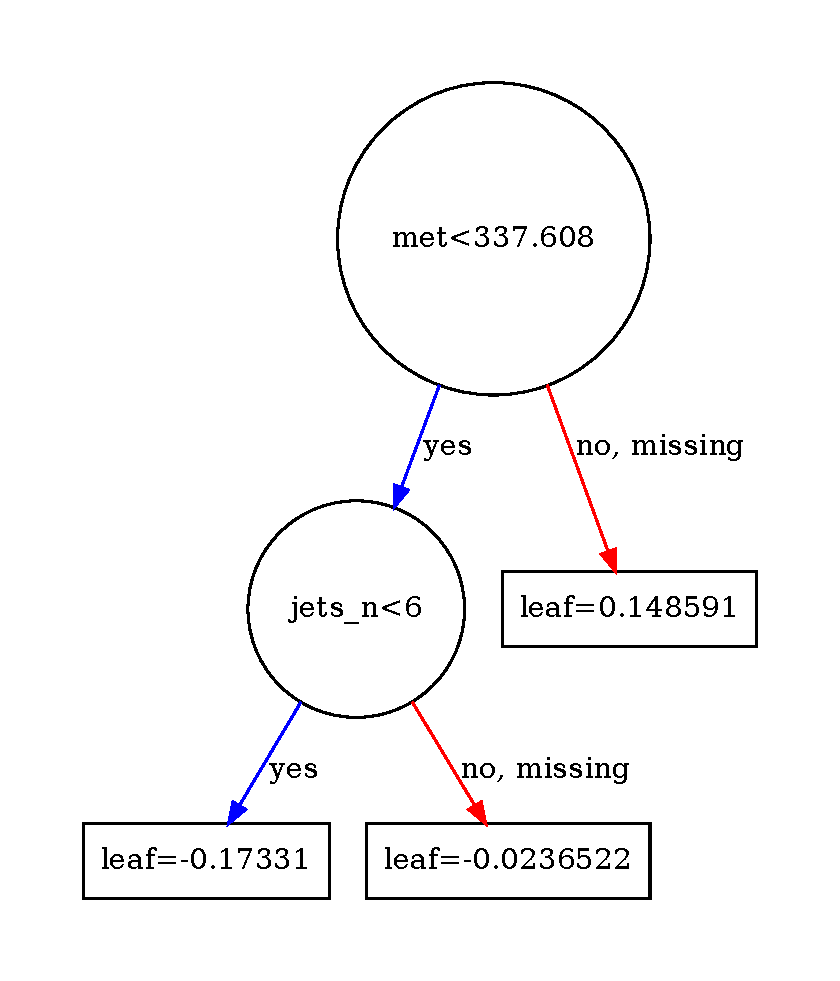
\includegraphics[width=0.4\textwidth]{figures/ml/tree7_g2000_n1200}
\caption{
Simple classification and regression tree (CART) on \num{2} variables
extracted from a \xgboost \cite{XGBoost} model.
Here signal-like (background-like) events receive positive (negative) weights in the leaves.
A logistic function is used to properly transform $w$ into a prediction
$\yhat = 1 /\left(1+e^{-w}\right)$ within $0 < \yhat < 1$.
}
\label{class:CART:small_example_CART}
\end{figure}

%%%%%%%%%%%%%%%%%%%%%%%%%%%%%%%%%%%%%%%%%%%%%%%%%%%%%%%%
\subsection{CART Training}
\label{class:CART:train}

CART models are almost always trained with greedy, \ie local, optimizers
that iteratively grow the tree from a root node.
At each node the optimal split $x_{j} < \beta_{\text{threshold}}$
over the available features is chosen according to a prespecified splitting criterion.
For classification trees, common choices for the splitting criterion are
the Gini impurity of \cref{class:CART:gini_impurity}
and Shannon entropy of \cref{class:CART:shannon_entropy},
while the MSE is used for regression trees.
The tree is constructed in this manner,
typically with recursive function calls,
until no additional splits are possible or
halting conditions set by hyperparameters are met such as
the minimum decrease in splitting criterion,
or the minimum number of training rows $\vb{x}_{i}$ at a node.

%%%%%%%%%%%%%%%%%%%%%%%%%%%%%%%%%%%%%%%%%%%%%%%%%%%%%%%%
\subsection{Gini Impurity}
\label{class:CART:gini_impurity}

The Gini impurity, or Gini index,
is the probability of incorrectly labeling a randomly selected element of set $S$,
when the label is chosen randomly according to the distribution of labeled elements in $S$.
Letting $p_{k}$ represent the proportion of elements labeled $k$ in $S$,
the Gini impurity\footnote{In binary classification with $K=2$,
\cref{eq:gini_impurity} $\to \, \text{Gini} = 2 p_{0} \left(1-p_{0}\right)$.} is then:

\begin{equation} \label{eq:gini_impurity}
\text{Gini} = \sum_{k=0}^{K-1} p_{k}\left(1-p_{k}\right) = 1 - \sum_{k=0}^{K-1} p_{k}^{2}.
\end{equation}

When $S$ only contains a single label the Gini impurity obtains its minimum value of \num{0};
any other `impure' $S$ will have $0 < \text{Gini}$.
When used as the splitting criterion,
the split at a node which maximizes the decrease in Gini impurity is selected.

%%%%%%%%%%%%%%%%%%%%%%%%%%%%%%%%%%%%%%%%%%%%%%%%%%%%%%%%
\subsection{Shannon Entropy}
\label{class:CART:shannon_entropy}
% TODO

\begin{equation} \label{eq:shannon_entropy}
H = -\sum_{k=0}^{K-1} p_{k} \log_{2}\left(p_{k}\right)
\end{equation}

% TODO equivalent to minimizing the log loss

%%%%%%%%%%%%%%%%%%%%%%%%%%%%%%%%%%%%%%%%%%%%%%%%%%%%%%%%
\subsection{CART Predictions}
\label{class:CART:pred}

To make a prediction for row $\vb{x}_{i}$
the tree and its branches are traversed
until of the terminating leaf is reached.
The prediction assigned by the leaf can be constructed in a few ways;
a class label may be assigned based on the majority class in the leaf during training,
a probability can be assigned based on the proportion of classes in the leaf,
or a weight $w$ can be computed from the loss function and training data in a more complex manner, \eg \xgboost \cite{XGBoost}.
Note that the leaf values can be trained separately from the tree structure
using an independent fold of the training data.
Tree models trained in this way are known as `honest' \cite{JMLR:v13:biau12a,pmlr-v32-denil14}.

%%%%%%%%%%%%%%%%%%%%%%%%%%%%%%%%%%%%%%%%%%%%%%%%%%%%%%%%
%%%%%%%%%%%%%%%%%%%%%%%%%%%%%%%%%%%%%%%%%%%%%%%%%%%%%%%%
\section{Boosted Decision Trees (BDT)}
\label{class:BDT}

Individual CARTs are rather poor and limited models
in terms of the behaviors they can successfully predict.
However, by taking an ensemble of $K$ complementary trees,
\ie boosting \cite{10.5555/3091696.3091715,FREUND1997119,Breiman1996BiasV,friedman2000} as described in \cref{ml_general:boosting},
and summing each CART's individual weight $w_{k}$ a much more flexible BDT\footnote{As the leaf weights
are reals rather than integer classes this approach may be better described as a boosted regression tree,
and can indeed handle regression problems without the logistic function.} is formed.
The component trees of a BDT are generated by iteratively adding new trees $f_{k}\left(x_{i}\right)$ to those which came before \cite{XGBoost},

\begin{equation} \label{eq:boosting}
\begin{aligned}
\yhat^{\left(0\right)} &= 0\,, \\
\yhat^{\left(1\right)} &= f_1\left(\mb{X}\right) = \yhat^{\left(0\right)} + f_1\left(\mb{X}\right), \\
\yhat^{\left(2\right)} &= f_1\left(\mb{X}\right) + f_2\left(\mb{X}\right)= \yhat^{\left(1\right)} + f_2\left(\mb{X}\right), \\
                           &\vdotswithin{\displaystyle =} \\
\yhat^{\left(t\right)} &= \sum_{k=1}^t f_k\left(\mb{X}\right)= \yhat^{\left(t-1\right)} + f_t\left(\mb{X}\right),
\end{aligned}
\end{equation}

\noindent where each tree $f_{k}$ is grown from zero branches while minimizing $S\left(\beta\right)$.
Through the ingenious use of a second order Taylor expansion this process can
be recast as a form of gradient descent\footnote{See \cite{NIPS1999_96a93ba8} for a different explanation.}, and thus is known as
stochastic gradient boosting \cite{10.2307/2699986,FRIEDMAN2002367}.
The number of boosting rounds, and thus trees, $K$ can be chosen in advance
but is better optimized during the training process via early stopping.

%%%%%%%%%%%%%%%%%%%%%%%%%%%%%%%%%%%%%%%%%%%%%%%%%%%%%%%%
\subsection{\xgboost}% would rather have the \textsc caps than italics
\label{class:BDT:xgboost}
% TODO see https://towardsdatascience.com/boosting-algorithm-xgboost-4d9ec0207d
% TODO how does the Hessian come into play

The \xgboost\footnote{\xgboost: eXtreme Gradient Boosting, \href{https://github.com/dmlc/xgboost}{github.com/dmlc/xgboost}.} library \cite{XGBoost}
is a modern open source implementation of gradient boosted decision tree methods.
Through various algorithmic and memory optimizations \xgboost demonstrates good performance\footnote{\xgboost has lost
its lead in recent years to newer libraries such as LightGBM \cite{LightGBM}
and CatBoost \cite{CatBoost}, but is still a standard library.}.
L1 and L2 regularization is incorporated via

\begin{equation} \label{eq:bdt_omega_reg}
\Omega\left(f\right) = \alpha T + \frac{1}{2}\lambda \sum_{j=1}^T w_j^2\,,
\end{equation}

\noindent where $T$ is the number of leaves in a tree and $w_{j}$ are the leaf weights;
however, the default hyperparameters $\alpha=0$ and $\lambda=1$ only enable L2 regularization.
Other important hyperparameters in \xgboost include the
learning rate $\eta$, which scales the corrections added by each new tree,
maximum tree depth, which sets a limit on the complexity of any tree via its depth,
and the early stopping validation threshold.
For reference $\eta=0.3$ and a maximum depth of 6 are the default values.

%%%%%%%%%%%%%%%%%%%%%%%%%%%%%%%%%%%%%%%%%%%%%%%%%%%%%%%%
\subsection{AdaBoost}
\label{class:BDT:AdaBoost}
% TODO

%%%%%%%%%%%%%%%%%%%%%%%%%%%%%%%%%%%%%%%%%%%%%%%%%%%%%%%%
%%%%%%%%%%%%%%%%%%%%%%%%%%%%%%%%%%%%%%%%%%%%%%%%%%%%%%%%
\section{Random Forest}
\label{class:RF}
% TODO

% TODO best results occur when you chose $\sqrt{n}$ features randomly to build each tree

%%%%%%%%%%%%%%%%%%%%%%%%%%%%%%%%%%%%%%%%%%%%%%%%%%%%%%%%
%%%%%%%%%%%%%%%%%%%%%%%%%%%%%%%%%%%%%%%%%%%%%%%%%%%%%%%%
\section{Fast Interpretable Greedy-Tree Sums (FIGS)}
\label{class:FIGS}

Fast Interpretable Greedy-Tree Sums (FIGS) \cite{FIGS,G-FIGS}
is an extension of the basic CART structure introduced in \cref{class:CART}.
Depending on the nature of the training data,
a CART will tend to reproduce subsets of the tree along different branches.
The resulting deep trees are not ideal as they contain many splits,
increasing the chance of fitting to noise in the data,
and because they have less data to work with at each subsequent split,
increasing the variance of the tree's predictions.

FIGS improves upon the CART iterative training process
by considering adding the next split as the root of a new tree,
in addition to adding the next split at the bottom of the existing tree as is done in CART.
This reduces the number of splits when the data has an additive structure,
as can be seen in \cref{class:FIGS:intro}, and increases interpretability.
The splits are chosen greedily according to the splitting criterion,
typically the Gini impurity of \cref{class:CART:gini_impurity}.
Each tree is fit to the residuals remaining after summing the other tree's predictions,
see \cref{class:FIGS:fit_algo} for an outline of the training algorithm.
Predictions are made by summing the predicted leaf's value\footnote{TODO value is just $p_{1} = n_{1}/N$?} from each tree.

\begin{figure}[H]
\centering
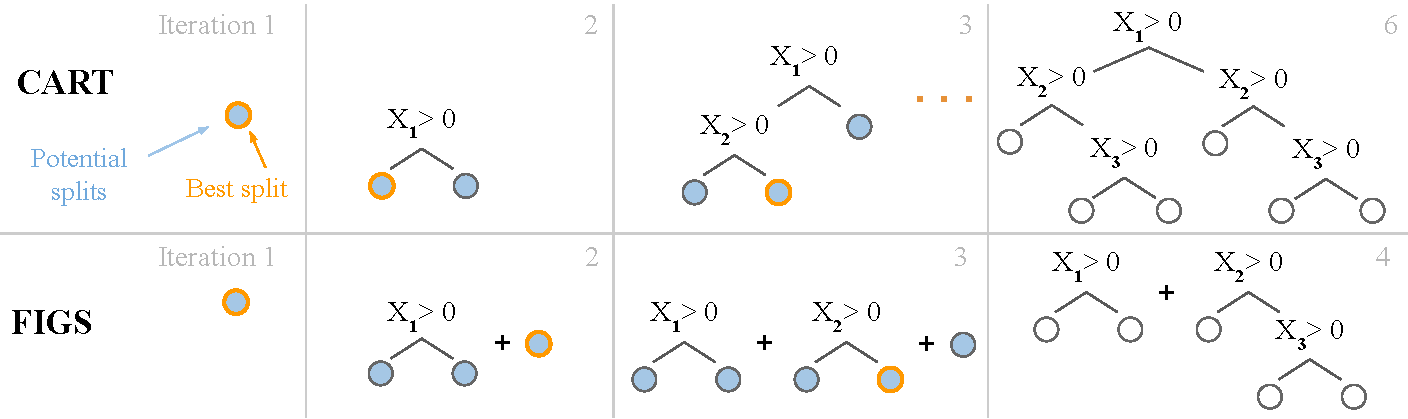
\includegraphics[width=\textwidth]{figures/ml/figs_intro_fig.pdf}
\caption{
A comparison of CART and FIGS tree growth on the toy dataset
$y = \identity_{x_{1} > 0} + \identity_{x_{2} > 0} \, \identity_{x_{3} > 0}$ \cite{FIGS}.
At each training iteration FIGS considers adding a new split at the bottom of the existing tree(s) like CART,
but also considers starting a new tree entirely.
Notice that CART must repeat the $x_{2}, x_{3}$ subtree on each side of the $x_{1}$ split,
while FIGS captures the additive structure of $y$ directly, thereby saving \num{2} splits.
}
\label{class:FIGS:intro}
\end{figure}

\begin{algorithm}[h]
  \caption{FIGS fitting algorithm, adapted from \cite{FIGS}.}
  \label{class:FIGS:fit_algo}
  \small
\begin{algorithmic}
  \State {FIGS}(X: features, y: outcomes, $\nu$: max\_splits)
  \State trees = []
  \While{count\_total\_splits(trees) $< \nu$:}
    \State all\_trees = join(trees, build\_new\_tree()) \textcolor{codegreen}{\# add new tree}
    \State potential\_splits = []
    \For{}\hspace{-3pt}tree in all\_trees:
        \State y\_residuals = y $-$ predict(all\_trees except tree)
        \For{}\hspace{-3pt}leaf in tree:
            \State potential\_split = split(X, y\_residuals, leaf)
            \State potential\_splits.append(potential\_split)
        \EndFor
    \EndFor
    \State best\_split = split\_with\_min\_impurity(potential\_splits)
    \State trees.insert(best\_split)
  \EndWhile
\end{algorithmic}
\end{algorithm}

The resulting FIGS model is thus an ensemble of CART-like trees,
similar to the BDT and RF models of \cref{class:BDT,class:RF}.
However, FIGS can capture any additive structure present in the data,
while the ensemble trees of the BDT (RF) model being trained sequentially (independently) can not.
Rather than constraining the depth or number of trees separately like other tree-based models,
FIGS can impose a limit on the total number of splits across all trees via the hyperparameter $\nu$.
This makes the construction of small, interpretable, models much easier.
Similar to CART, FIGS can also set hyperparameters for
the minimum decrease in impurity and
number of features to consider at each split.
With $\nu < 20$, readily interpretable FIGS models have been observed
to have state-of-the-art performance on multiple datasets \cite{FIGS}.

A \python implementation of the FIGS algorithm can be found in the \texttt{imodels} package \cite{imodels}.
The FIGS training time goes as $\order{n \, \nu^{2} m^{2}}$ \cite{FIGS},
where $n$ is the number of features and $m$ is the number of data points,
which is quite fast on a modern machine for reasonable $m$, even when $n$ is large.

% TODO add dtreeviz illustration

%%%%%%%%%%%%%%%%%%%%%%%%%%%%%%%%%%%%%%%%%%%%%%%%%%%%%%%%
%%%%%%%%%%%%%%%%%%%%%%%%%%%%%%%%%%%%%%%%%%%%%%%%%%%%%%%%
\section{\texorpdfstring{$k$}{k}-Nearest Neighbors (\texorpdfstring{$k$}{k}-NN)}
\label{class:kNN}
% TODO
% TODO \kNN

%%%%%%%%%%%%%%%%%%%%%%%%%%%%%%%%%%%%%%%%%%%%%%%%%%%%%%%%
%%%%%%%%%%%%%%%%%%%%%%%%%%%%%%%%%%%%%%%%%%%%%%%%%%%%%%%%
\section{Artificial Neural Networks (NN)}
\label{class:ANN}
% TODO

% TODO add back prop somewhere, here or in grad descent

\begin{figure}[H]
  \centering
  \begin{subfigure}[b]{0.48\textwidth}\centering
      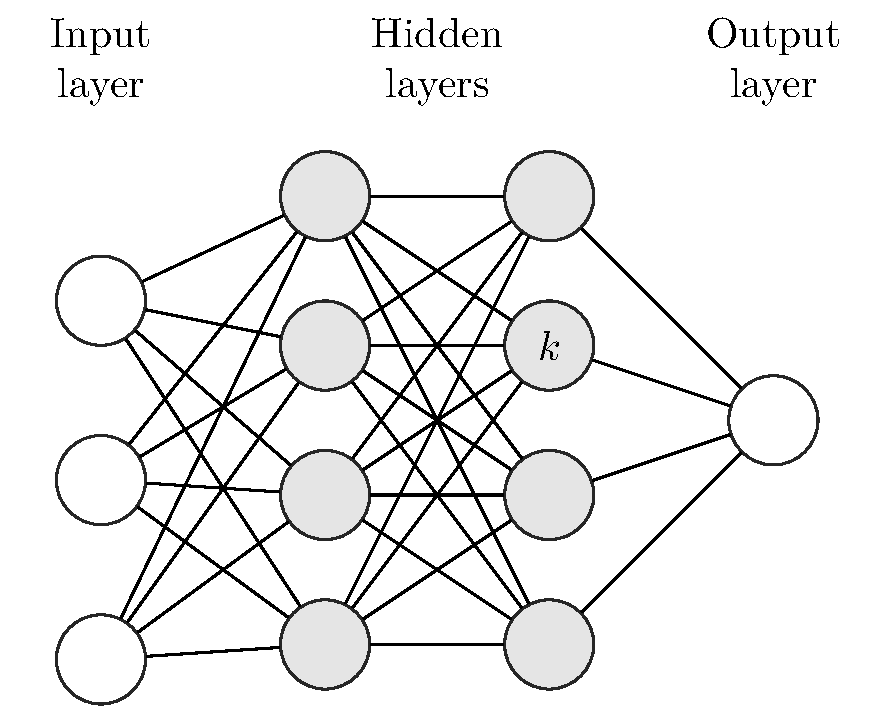
\includegraphics[width=\textwidth]{figures/ml/NN_diagram/NN_diagram}
  \caption{NN Example}
  \label{fig:NN:ex}
  \end{subfigure}
  ~
  \begin{subfigure}[b]{0.48\textwidth}\centering
      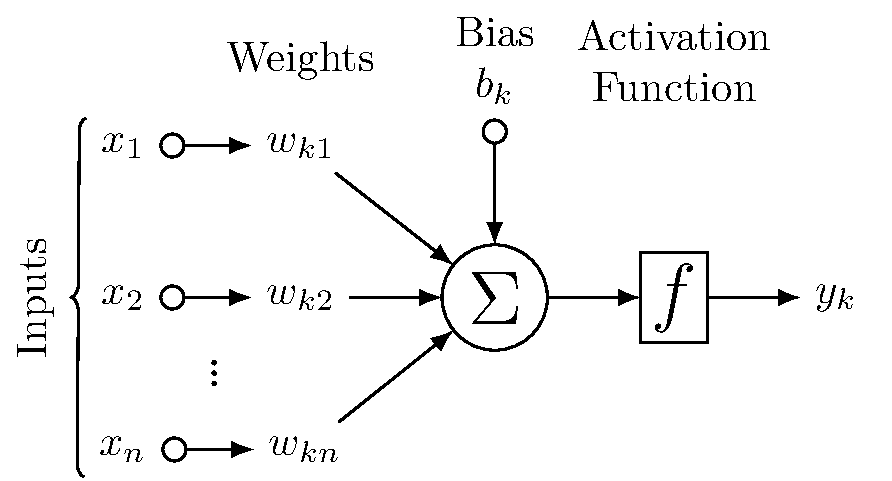
\includegraphics[width=\textwidth]{figures/ml/NN_neuron/NN_neuron}
  \caption{Neuron}
  \label{fig:NN:Neuron}
  \end{subfigure}
\caption{
Illustrations of the components of a neural network.
\label{fig:NN}
}
\end{figure}

%%%%%%%%%%%%%%%%%%%%%%%%%%%%%%%%%%%%%%%%%%%%%%%%%%%%%%%%
%%%%%%%%%%%%%%%%%%%%%%%%%%%%%%%%%%%%%%%%%%%%%%%%%%%%%%%%
\section{Recursive Neural Networks (RNN)}
\label{class:RNN}
% TODO

%%%%%%%%%%%%%%%%%%%%%%%%%%%%%%%%%%%%%%%%%%%%%%%%%%%%%%%%
\subsection{Long Short Term Memory (LSTM)}
\label{class:RNN:LSTM}
% TODO

%%%%%%%%%%%%%%%%%%%%%%%%%%%%%%%%%%%%%%%%%%%%%%%%%%%%%%%%
%%%%%%%%%%%%%%%%%%%%%%%%%%%%%%%%%%%%%%%%%%%%%%%%%%%%%%%%
\section{Convolutional Neural Networks (CNN)}
\label{class:CNN}
% TODO

%%%%%%%%%%%%%%%%%%%%%%%%%%%%%%%%%%%%%%%%%%%%%%%%%%%%%%%%
%%%%%%%%%%%%%%%%%%%%%%%%%%%%%%%%%%%%%%%%%%%%%%%%%%%%%%%%
\section{Learning Vector Quantization (LVQ)}
\label{class:kNN:LVQ}
% TODO

%%%%%%%%%%%%%%%%%%%%%%%%%%%%%%%%%%%%%%%%%%%%%%%%%%%%%%%%
%%%%%%%%%%%%%%%%%%%%%%%%%%%%%%%%%%%%%%%%%%%%%%%%%%%%%%%%
\section{Addressing Class Imbalance}
\label{class:imbalance}
% TODO

TODO \cref{ml_general:eval:class_priors}
}
%%%%%%%%%%%%%%%%%%%%%%%%%%%%%%%%%%%%%%%%%%%%%%%%%%%%%%%%
%%%%%%%%%%%%%%%%%%%%%%%%%%%%%%%%%%%%%%%%%%%%%%%%%%%%%%%%
%%%%%%%%%%%%%%%%%%%%%%%%%%%%%%%%%%%%%%%%%%%%%%%%%%%%%%%%
\chapter{Clustering}
\label{chap:cluster}

%%%%%%%%%%%%%%%%%%%%%%%%%%%%%%%%%%%%%%%%%%%%%%%%%%%%%%%%
%%%%%%%%%%%%%%%%%%%%%%%%%%%%%%%%%%%%%%%%%%%%%%%%%%%%%%%%
\section{Evaluating Performance}
\label{cluster:eval}
% TODO

%%%%%%%%%%%%%%%%%%%%%%%%%%%%%%%%%%%%%%%%%%%%%%%%%%%%%%%%
\subsection{Davies-Bouldin Index}
\label{cluster:eval:davies_bouldin}
% TODO

\begin{equation} \label{eq:davies_bouldin}
\text{DB} = \frac{1}{m} \sum_{i=1}^{m} \max_{i \neq j} \left(\frac{\sigma_{i} + \sigma_{j}}{\abs{\vb{c}_{i} - \vb{c}_{j}}}\right)
\end{equation}

%%%%%%%%%%%%%%%%%%%%%%%%%%%%%%%%%%%%%%%%%%%%%%%%%%%%%%%%
\subsection{Adjusted Rand Index}
\label{cluster:eval:adjusted_rand_index}
% TODO

%%%%%%%%%%%%%%%%%%%%%%%%%%%%%%%%%%%%%%%%%%%%%%%%%%%%%%%%
\subsection{Shannon Index}
\label{cluster:eval:shannon_index}
% TODO

%%%%%%%%%%%%%%%%%%%%%%%%%%%%%%%%%%%%%%%%%%%%%%%%%%%%%%%%
\subsection{Silhouette Coefficient}
\label{cluster:eval:silhouette}
% TODO

%%%%%%%%%%%%%%%%%%%%%%%%%%%%%%%%%%%%%%%%%%%%%%%%%%%%%%%%
%%%%%%%%%%%%%%%%%%%%%%%%%%%%%%%%%%%%%%%%%%%%%%%%%%%%%%%%
\section{\texorpdfstring{$k$}{k}-Means}
\label{cluster:kMean}
% TODO

%%%%%%%%%%%%%%%%%%%%%%%%%%%%%%%%%%%%%%%%%%%%%%%%%%%%%%%%
\subsection{Choosing \texorpdfstring{$k$}{k}: Elbow Method}
\label{cluster:kMean:elbow}
% TODO

%%%%%%%%%%%%%%%%%%%%%%%%%%%%%%%%%%%%%%%%%%%%%%%%%%%%%%%%
\subsection{Metrics}
\label{cluster:kMean:metrics}
% TODO

\subsubsection{Cartesian Radius}
\label{cluster:kMean:metrics:cartesian}
% TODO

% \begin{equation}\label{eq:cartesian}
% \end{equation}

\subsubsection{Cosine Simularity}
\label{cluster:kMean:metrics:cos}
% TODO

% \begin{equation}\label{eq:cos}
% \end{equation}

%%%%%%%%%%%%%%%%%%%%%%%%%%%%%%%%%%%%%%%%%%%%%%%%%%%%%%%%
%%%%%%%%%%%%%%%%%%%%%%%%%%%%%%%%%%%%%%%%%%%%%%%%%%%%%%%%
\section{Expectation Maximization (EM)}
\label{cluster:EM}
% TODO

%%%%%%%%%%%%%%%%%%%%%%%%%%%%%%%%%%%%%%%%%%%%%%%%%%%%%%%%
\subsection{Gaussian Mixture Model (GMM)}
\label{cluster:EM:GMM}
% TODO

%%%%%%%%%%%%%%%%%%%%%%%%%%%%%%%%%%%%%%%%%%%%%%%%%%%%%%%%
%%%%%%%%%%%%%%%%%%%%%%%%%%%%%%%%%%%%%%%%%%%%%%%%%%%%%%%%
\section{Louvain Method}
\label{cluster:louvain}

When working with a graph, \ie network, based dataset
we can use the Louvain\footnote{Named for the location of the author's university in Louvain-la-Neuve, Belgium.} method \cite{louvain}
to detect related clusters, \ie communities,
of nodes by optimizing the graph's modularity\footnote{Today the Louvain method can refer to the greedy optimization algorithm on its own,
with the modularity $Q$ being one possible objective function}.
The modularity $Q$ of a graph $G$ with a given set of clusters $C$
is a measure of the graph's degree of clustering;
being the fraction of edges within the clusters
minus the expected fraction if the edges were randomly distributed.
In short, we can think of $Q$ as a measure of
the density of interior to exterior edges of the clusters.
$Q$ ranges from \num{-0.5} for relatively uncluttered graphs
to \num{1} for fully clustered graphs.
We can compute the modularity $Q$ of $G$ as:

\begin{equation} \label{eq:unsupervised:louvain:modularity}
Q\left(G\right) = \frac{1}{2 W_{G}} \sum_{ij \in G} \bigg(w_{ij} - \gamma \frac{W_{i} W_{j}}{2 W_{G}}\bigg) \delta\left(c_{i},\,c_{j}\right)
\end{equation}

\noindent where\footnote{Note $w_{ij}=1$ for an unweighted graph, and $2 W_{G} = \sum_{ij \in G} w_{ij}$ accounts for double counting edges.}
$w_{ij}$ is the edge weight between nodes $i$ and $j$,
$W_{i}$ is the sum of edge weights of node $i$,
$W_{G}$ is the total edge weight of the graph,
$c_{i} \in C$ is the cluster of node $i$,
and $0 < \gamma$ is a resolution hyperparameter.

The Louvain method constructs $C$ by greedily maximizing $Q$ in an iterative two phase process as shown in \cref{fig:louvain}.
In the first phase, we define each node $n_{i} \in G$ to be its own cluster $c_{i}$.
We then merge each $c_{i}$ with the neighboring $c_{j}$, $0 < w_{ij}$, which maximizes $\Delta Q$.
If $\max\left(\Delta Q\right) = 0$ we leave $c_{i}$ unmerged.
After all clusters have been merged and $Q$ is at a local maximum we enter the second phase.
Here a new graph $G'$ is constructed by making each cluster $c_{i}$ into a node $n'_{i} \in G'$.
The old weights of $G$ are summed to become the new weights $w'_{ij}$,
with intra-cluster weights becoming self-loops $w'_{ii}$ in $G'$.
We return to the first phase and repeat until $Q$ has been maximized.

\begin{figure}
\centering
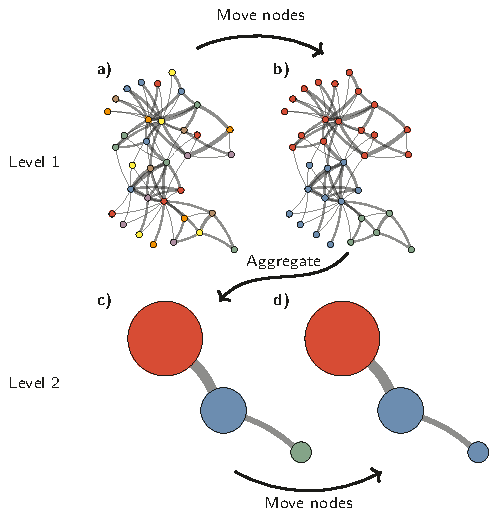
\includegraphics[width=0.5\textwidth]{figures/ml/louvain_algo}
\caption{
Illustration of the two iterative phases of the Louvain method \cite{leiden}.
}
\label{fig:louvain}
\end{figure}

The resolution parameter $\gamma$ controls the number and size of clusters, $\gamma =1$ by default.
The location of $\gamma$ depends on the text and implementation,
but here $1 < \gamma$ ($\gamma < 1$) favors more (fewer) clusters with fewer (more) constituent nodes.
The \texttt{python-louvain}
\href{https://python-louvain.readthedocs.io/en/latest/}{package} \cite{python-louvain}
implements the Louvain method for \texttt{networkx} \cite{networkx}
\href{https://networkx.org/}{based graphs}.
Community detection in large networks is an important problem for social networks and other use cases,
making this an active area of research.
For example, one proposed improvement to the Louvain method is the Leiden algorithm \cite{leiden}.

%%%%%%%%%%%%%%%%%%%%%%%%%%%%%%%%%%%%%%%%%%%%%%%%%%%%%%%%
%%%%%%%%%%%%%%%%%%%%%%%%%%%%%%%%%%%%%%%%%%%%%%%%%%%%%%%%
\section{Correlation Clustering}
\label{cluster:correlation}
% TODO

%%%%%%%%%%%%%%%%%%%%%%%%%%%%%%%%%%%%%%%%%%%%%%%%%%%%%%%%
%%%%%%%%%%%%%%%%%%%%%%%%%%%%%%%%%%%%%%%%%%%%%%%%%%%%%%%%
\section{Affinity Clustering}
\label{cluster:affinity}
% TODO

%%%%%%%%%%%%%%%%%%%%%%%%%%%%%%%%%%%%%%%%%%%%%%%%%%%%%%%%
%%%%%%%%%%%%%%%%%%%%%%%%%%%%%%%%%%%%%%%%%%%%%%%%%%%%%%%%
\section{Support Vector Clustering}
\label{cluster:SVC}
% TODO

}
%%%%%%%%%%%%%%%%%%%%%%%%%%%%%%%%%%%%%%%%%%%%%%%%%%%%%%%%
%%%%%%%%%%%%%%%%%%%%%%%%%%%%%%%%%%%%%%%%%%%%%%%%%%%%%%%%
%%%%%%%%%%%%%%%%%%%%%%%%%%%%%%%%%%%%%%%%%%%%%%%%%%%%%%%%
\chapter{Time Series Analysis}
\label{chap:time_series}
% https://www.youtube.com/playlist?list=PLvcbYUQ5t0UHOLnBzl46_Q6QKtFgfMGc3

Time series analysis is the study of time-dependent data such as price over time.
Similar to regression models we aim to fit a model
to the data in order to make future predictions.
However, instead of interpolating within a range of previously observed data points,
time series aims to extrapolate from our current data into the future,
as we are not interested in making predictions about past dates.
As we extrapolate further and further away from observed data
the uncertainty of our predictions will naturally grow,
making time series a harder problem to address than normal regression.
There are a variety of potential models to choose from,
each with their own assumptions and use cases.
The problem can be attacked from two general directions,
frequency-domain methods and time-domain methods,
but we shall focus primarily on the time-domain here.
The \texttt{statsmodels} \python \href{https://www.statsmodels.org}{module}
is very useful for implementing these modeling methods,
which will be referenced as appropriate.

\subsubsection{Lag Notation}
\label{time_series:L}

When working with time series data we often index time steps as $t$, $t-1$, $t-2$,\,\ldots\,
where $t$ is the current time.
The value of the variable in question, price, quantity, \etc,
at time $t$ is then $y_{t}$, with $y_{t-1}$, $y_{t-2}$,\,\ldots\, at subsequent times.
Instead of writing subscripts, sometimes it is more convenient
to switch to a polynomial based notation using
the lag operator $L$, also known as the backshift operator $B$ in some texts:

\begin{equation}\label{eq:time_series:L}
L y_{t} = y_{t-1},\quad L^{2} y_{t} = y_{t-2},\,\ldots \quad L^{k} y_{t} = y_{t-k}.
\end{equation}

%%%%%%%%%%%%%%%%%%%%%%%%%%%%%%%%%%%%%%%%%%%%%%%%%%%%%%%%
%%%%%%%%%%%%%%%%%%%%%%%%%%%%%%%%%%%%%%%%%%%%%%%%%%%%%%%%
\section{Correlation in Time Series}
\label{time_series:correlation}

In time series analysis $y_{t}$ can depend, to varying degree,
on the previous values $L^{k} y_{t},\, \forall k$.
There is a direct component to this dependence,
$y_{t} \sim f\left(y_{t-1}\right)$,
but also an indirect or recursive component,
$y_{t} \sim f\left(y_{t-1}\right) \sim f\left(g\left(y_{t-2}\right)\right)$.

%%%%%%%%%%%%%%%%%%%%%%%%%%%%%%%%%%%%%%%%%%%%%%%%%%%%%%%%
\subsection{Auto-Correlation Function (ACF)}
\label{time_series:ACF}

Neglecting the multiple components of the correlation of $y_{t}$ with prior times,
we can commute the overall auto-correlation function (ACF) of $y_{t}$
with itself at some amount of lag $k$ as

\begin{equation}\label{eq:time_series:ACF}
\text{ACF}\left(y,k\right) = \corr{y_{t}}{y_{t-k}},
\end{equation}

\noindent using the regular Pearson correlation coefficient \cref{eq:stats:corr:pearson}.
The auto-correlation shows the total correlation and is simple to compute,
but mixes the direct and indirect effects of prior values together.

%%%%%%%%%%%%%%%%%%%%%%%%%%%%%%%%%%%%%%%%%%%%%%%%%%%%%%%%
\subsection{Partial Auto-Correlation Function (PACF)}
\label{time_series:PACF}

In contrast, partial auto-correlation function
aims to isolate the direct influence of $y_{t-k}$ on $y_{t}$ for some lag $k$.
We can get at this component by fitting $y_{t}$ as a linear function of $L^{n} y_{t}$,

\begin{equation}\label{eq:time_series:PACF}
y_{t} = \sum_{i=1}^{k} \phi_{k,i}\, y_{t-i} + \epsilon_{k},
\end{equation}

\noindent and identifying $\text{PACF}\left(y,k\right) = \phi_{k,k}$
as the partial auto-correlation function for $k$.
Note that for each $k$, we need to do a new fit of \cref{eq:time_series:PACF},
and after fitting should check that $\phi_{k,k}$ is statistically significant,
\ie we reject $H_{0}$ that $\phi_{k,k}=0$, by looking at the coefficient's confidence interval from the fit.
We can generate plots of ACF and PACF versus $k$ to explore a time series
with the \texttt{plot\_acf} and \texttt{plot\_pacf}
\href{https://www.statsmodels.org/stable/graphics.html\#time-series-plots}{functions}.

%%%%%%%%%%%%%%%%%%%%%%%%%%%%%%%%%%%%%%%%%%%%%%%%%%%%%%%%
%%%%%%%%%%%%%%%%%%%%%%%%%%%%%%%%%%%%%%%%%%%%%%%%%%%%%%%%
\section{Stationarity}
\label{time_series:stationarity}

Stationarity is an important assumption for many parametric time series models,
which combines three properties:

\begin{enumerate}[noitemsep]
  \item The mean $\expval{y}$ of the time series is constant, \ie the average is not moving.\label{item:time_series:stationarity:constant_mean}
  \item The variance $\variance{y}$ of the time series is constant.\label{item:time_series:stationarity:constant_var}
  \item The time series does not exhibit seasonality, \ie no periodic fluctuations in $y\left(t\right)$.\label{item:time_series:stationarity:seasonality}
\end{enumerate}

If the mean or variance is growing with time
we can look at the first difference, $\widetilde{y}_{t} = y_{t} - y_{t-1}$,
and see if the time series of $\widetilde{y}_{t}$ is stationary,
see \cref{time_series:I} for more.
Similarly, we can try to remove seasonality
by subtracting a deterministic time-dependent function $f\left(t\right)$
or by using the SARIMA model of \cref{time_series:SARIMA}.
We can also try normalizing with a \Zscore to address a changing mean or variance;
subtracting or dividing as needed to make the series more stationary.
This even works with seasonality if we subtract the mean value per medium-sized time unit, \eg month, quarter, \etc.
When cleaning the data in this way,
we will need to invert any preprocessing steps
while making predictions to return to the original units.

Simply looking at the graph of a time series can give us
a good intuition on if it is stationary or not.
However, we can formally test for stationarity
with the augmented Dickey--Fuller test (ADF) of \cref{time_series:ADF}.

%%%%%%%%%%%%%%%%%%%%%%%%%%%%%%%%%%%%%%%%%%%%%%%%%%%%%%%%
%%%%%%%%%%%%%%%%%%%%%%%%%%%%%%%%%%%%%%%%%%%%%%%%%%%%%%%%
\section{White Noise}
\label{time_series:white_noise}

In the context of time series analysis, white noise is random fluctuations which
have mean zero, $\expval{y} = 0$,
constant variance with respect to time, $\partial_{t} \variance{y} = 0$,
and no correlation between lags, $\corr{y_{t}}{y_{t-k}} = 0,\,\, \forall k$.
Ideally after fitting a time series, we will capture all of the signal
in the model and the resulting error term $\epsilon$ will only contain white noise.
We can test for white noise by looking at the moving average and ACF plot,
or more formally with the Ljung--Box test of \cref{time_series:ljung_box}.

%%%%%%%%%%%%%%%%%%%%%%%%%%%%%%%%%%%%%%%%%%%%%%%%%%%%%%%%
%%%%%%%%%%%%%%%%%%%%%%%%%%%%%%%%%%%%%%%%%%%%%%%%%%%%%%%%
\section{Autoregressive (AR) Models}
\label{time_series:AR}
Building on the PACF, we can construct an autoregressive (AR) model $\text{AR}\left(p\right)$
as a linear combination of lag components of the time series:

\begin{equation}\label{eq:time_series:AR}
\yhat_{t} = \phi_{0} + \sum_{i=1}^{p} \phi_{i}\, y_{t-i} + \epsilon_{t}.
\end{equation}

Note that we should look at the PACF plot before fitting \cref{eq:time_series:AR}
to determine which lags to include,
\ie set $p$ and decide which lags to skip\footnote{It may not be possible
to specify individual lags to include in some software packages,
but excluding non-significant coefficients and reducing model complexity
is still a good idea if possible.} by setting $\phi_{i} = 0$.

%%%%%%%%%%%%%%%%%%%%%%%%%%%%%%%%%%%%%%%%%%%%%%%%%%%%%%%%
%%%%%%%%%%%%%%%%%%%%%%%%%%%%%%%%%%%%%%%%%%%%%%%%%%%%%%%%
\section{Moving Average (MA) Models}
\label{time_series:MA}

Instead of looking at the auto-correlation $y_{y-i}$,
we can also build a time series model around
correcting for prior errors in the prediction,
\ie fitting to the moving average (MA).
The $\text{MA}\left(q\right)$ model
is then:

\begin{subequations}\label{eq:time_series:MA}
\begin{align}
\yhat_{t} &= \theta_{0} + \sum_{i=1}^{q} \theta_{i}\, \epsilon_{t-i} + \epsilon_{t}, \label{eq:time_series:MA_y} \\
\epsilon_{t-1} &= y_{t-1} - \yhat_{t-1}. \label{eq:time_series:MA_epsilon}
\end{align}
\end{subequations}

Note that a $\text{MA}\left(q\right)$ model will fluctuate around the initial average $\theta_{0}$,
and can only predict $q$ steps into the future before constantly returning $\theta_{0}$.
We can select $q$ by looking at the ACF plot
and identifying the last non-zero lag.

%%%%%%%%%%%%%%%%%%%%%%%%%%%%%%%%%%%%%%%%%%%%%%%%%%%%%%%%
%%%%%%%%%%%%%%%%%%%%%%%%%%%%%%%%%%%%%%%%%%%%%%%%%%%%%%%%
\section{Invertibility of Time Series}
\label{time_series:invert}
% https://youtu.be/QU_VNu3rJKY
% https://youtu.be/q0vz7dGlZL0

One interesting property of AR and MA time series models is their invertibility:

\begin{subequations}\label{eq:time_series:invert}
\begin{align}
\text{MA}\left(1\right) &= \text{AR}\left(\infty\right), \label{eq:time_series:invert:MA_1} \\
\text{AR}\left(1\right) &= \text{MA}\left(\infty\right). \label{eq:time_series:invert:AR_1}
\end{align}
\end{subequations}

For a proof of \cref{eq:time_series:invert:MA_1}, see \cref{eq:time_series:invert_proof}.
Letting $\theta = \phi < 0$ for convenience and
assuming\footnote{Here we are assuming the time series is stationary, \ie no unit roots $\abs{\phi} < 1$.} $\abs{\phi} < 1$
we can construct the time series $C_{t}$,

\begin{subequations}\label{eq:time_series:invert_proof}
\begin{align}
C_{t} \equiv \text{MA}\left(1\right) - \theta_{0} &= -\phi\, \epsilon_{t-1} + \epsilon_{t} = \left(1 - \phi L \right) \epsilon_{t}, \label{eq:time_series:invert_proof:a} \\
\implies \epsilon_{t} &= \frac{C_{t}}{1 - \phi L}, \label{eq:time_series:invert_proof:b} \\
&= \left(\,\sum_{i=0}^{\infty} \phi^{i} L^{i} \right) C_{t} = \sum_{i=0}^{\infty} \phi^{i} C_{t-i}, \label{eq:time_series:invert_proof:c} \\
\implies C_{t} &= \sum_{i=1}^{\infty} -\phi^{i} C_{t-i} + \epsilon_{t} = \text{AR}\left(\infty\right) - \phi_{0}, \label{eq:time_series:invert_proof:d}
\end{align}
\end{subequations}

\noindent where in \cref{eq:time_series:invert_proof:c} we have used
the sum of a geometric series \cref{eq:misc:math:geometric}.
The proof of \cref{eq:time_series:invert:AR_1} is similar and also relies on the geometric series.
Essentially we are making the recursive nature of these time series explicit and using it to transform from one to the other.
The $\text{AR}\left(\infty\right)$ expansion of $\text{MA}\left(1\right)$
is particularly useful as it is possible in practice to truncate the series at $\order{\phi^{\,p}}$
where $\phi^{\,p} \approx 0$ and represent $\text{MA}\left(1\right)$ as
a pure function of the time series itself, \ie without recursion.

%%%%%%%%%%%%%%%%%%%%%%%%%%%%%%%%%%%%%%%%%%%%%%%%%%%%%%%%
%%%%%%%%%%%%%%%%%%%%%%%%%%%%%%%%%%%%%%%%%%%%%%%%%%%%%%%%
\section{ARMA Model}
\label{time_series:ARMA}

While we can represent AR $\Leftrightarrow$ MA with infinite series,
it is more practical to include both in one model with a finite number of terms.
The $\text{ARMA}\left(p,q\right)$ model is a simple combination of
both approaches:

\begin{equation}\label{eq:time_series:ARMA}
\yhat_{t} = \mu_{0} + \sum_{i=1}^{p} \phi_{i}\, y_{t-i} + \sum_{i=1}^{q} \theta_{i}\, \epsilon_{t-i} + \epsilon_{t}.
\end{equation}

Using lag notation we can write \cref{eq:time_series:ARMA} more
compactly\footnote{We drop
the constant intercept terms for convenience, as do many other sources.
However a constant term can still be included if desired,
or we can construct $\widetilde{y}_{t} = y_{t} - \mu_{0}$ with $\expval{\widetilde{y}_{t}} = 0$.}\footnote{If we set
$\phi_{0}=-1$, $\theta_{0} = 1$ and start the sums at $i=0$
we can simplify \cref{eq:time_series:ARMA_lag} even further.} as

\begin{subequations}\label{eq:time_series:ARMA_lag}
\begin{align}
\phi\left(L,p\right) y_{t} &= \theta\left(L,q\right) \epsilon_{t}, \label{eq:time_series:ARMA_lag:def} \\
\phi\left(L,p\right) &= 1 - \sum_{i=1}^{p} \phi_{i}\, L^{i}, \label{eq:time_series:ARMA_lag:phi} \\
\theta\left(L,q\right) &= 1 + \sum_{i=1}^{q} \theta_{i}\, L^{i}, \label{eq:time_series:ARMA_lag:theta}
\end{align}
\end{subequations}

\noindent where \cref{eq:time_series:ARMA_lag:phi,eq:time_series:ARMA_lag:theta} are polynomials of the lag operator $L$.
To avoid parameter redundancy, \ie multiple $\phi$, $\theta$ coefficients for $\order{L^{n}}$,
we require the polynomials $\phi\left(L,p\right)$ and $\theta\left(L,q\right)$ to not share any common factors.

%%%%%%%%%%%%%%%%%%%%%%%%%%%%%%%%%%%%%%%%%%%%%%%%%%%%%%%%
%%%%%%%%%%%%%%%%%%%%%%%%%%%%%%%%%%%%%%%%%%%%%%%%%%%%%%%%
\section{Integrated (I) Models}
\label{time_series:I}

The previous models have worked well for stationary time series with constant means,
however we may wish to model a quantity with a mean that linearly changes over time.
One method of incorporating this behavior in a time series model is by
recursively taking the difference $d$ times between lags of the original time series $y_{t}$
to construct a new time series $\widetilde{y}_{t}$ \cref{eq:time_series:I:forward}.
With the appropriate choice of $d$, typically $d \leq 2$,
$\widetilde{y}_{t}$ should have a constant mean,
allowing other models to be subsequently used.
This process is known as the integrated model $\text{I}\left(d\right)$,
though the name is misleading as what we are really doing is differentiating $y$ to find a constant slope, curvature, \etc.
Note, when making predictions we will need to
transform back to the original $y_{t}$ \cref{eq:time_series:I:backward1,eq:time_series:I:backward2},
at the cost of $d$ initial data points where no predictions can be made.

\begin{subequations}\label{eq:time_series:I}
\begin{align}
\widetilde{y}_{t} &= \left(1-L\right)^{d} y_{t}, \label{eq:time_series:I:forward} \\
y_{t} &= \widetilde{y}_{t} + y_{t-1},\,\, \text{where}\,\, d=1, \label{eq:time_series:I:backward1} \\
y_{t} &= \widetilde{y}_{t} + 2 y_{t-1} - y_{t-2},\,\, \text{where}\,\, d=2. \label{eq:time_series:I:backward2}
\end{align}
\end{subequations}

%%%%%%%%%%%%%%%%%%%%%%%%%%%%%%%%%%%%%%%%%%%%%%%%%%%%%%%%
%%%%%%%%%%%%%%%%%%%%%%%%%%%%%%%%%%%%%%%%%%%%%%%%%%%%%%%%
\section{ARIMA Model}
\label{time_series:ARIMA}

Putting everything together, we can construct the $\text{ARIMA}\left(p,d,q\right)$ model
by including \cref{eq:time_series:I:forward} in \cref{eq:time_series:ARMA_lag}:

\begin{equation}\label{eq:time_series:ARIMA}
\phi\left(L,p\right) \left(1-L\right)^{d} y_{t} = \theta\left(L,q\right) \epsilon_{t}.
\end{equation}

%%%%%%%%%%%%%%%%%%%%%%%%%%%%%%%%%%%%%%%%%%%%%%%%%%%%%%%%
\subsection{ARIMA Model Example}
\label{time_series:ARIMA:ex}

% TODO include example plots of y_{t}, PACF, ACF, predictions, and residuals; and link to the example notebook

%%%%%%%%%%%%%%%%%%%%%%%%%%%%%%%%%%%%%%%%%%%%%%%%%%%%%%%%
%%%%%%%%%%%%%%%%%%%%%%%%%%%%%%%%%%%%%%%%%%%%%%%%%%%%%%%%
\section{Seasonal ARIMA Model (SARIMA)}
\label{time_series:SARIMA}

Extending the ideas of the integrated model from \cref{time_series:I},
we can attempt to control for seasonality by
taking lags across $m$ time steps at once, \ie using $L^{m}$ in place of $L$.
For example, if $m=12$ corresponds to 1 year,
we will be doing the normal extrapolation of ARIMA on $y_{t-1-1\,\text{Year}}$ instead of $y_{t-1}$,
thereby canceling out any yearly periodic trends.
The resulting $\text{SARIMA}\left(p,d,q\right)\left(P,D,Q\right)_{m}$ model
has the normal $\text{ARIMA}\left(p,d,q\right)$ model components,
plus an additional set\footnote{Details around
coefficient conditions and parameter redundancy are omitted for brevity.} of uppercase parameters
controlling a $L^{m}$ based ARIMA model:

\begin{equation}\label{eq:time_series:SARMA}
\phi\left(L,p\right) \Phi\left(L^{m},P\right) \left(1-L\right)^{d} \left(1-L^{m}\right)^{D} y_{t} = \theta\left(L,q\right) \theta\left(L^{m},q\right) \epsilon_{t}.
\end{equation}

The $\text{SARIMA}\left(p,d,q\right)\left(P,D,Q\right)_{m}$ family of models
is available via the \texttt{ARIMA}
\href{https://www.statsmodels.org/stable/generated/statsmodels.tsa.arima.model.ARIMA.html}{class},
with a wide variety of attributes and methods
enabling us to implement all of the above time series models.
Computationally, \texttt{ARIMA} preforms fits via maximum likelihood estimation (MLE),
but AR models can also be fit with ordinary least squares (OLS).

%%%%%%%%%%%%%%%%%%%%%%%%%%%%%%%%%%%%%%%%%%%%%%%%%%%%%%%%
%%%%%%%%%%%%%%%%%%%%%%%%%%%%%%%%%%%%%%%%%%%%%%%%%%%%%%%%
\section{ARMA Model with Exogenous Inputs (ARMAX)}
\label{time_series:ARMAX}

The $\text{ARMAX}\left(p,q,b\right)$ model
extends ARMA by incorporating exogenous (X) inputs
via another known time series $d_{t}$:

\begin{equation}\label{eq:time_series:ARMAX}
\yhat_{t} = \mu_{0} + \sum_{i=1}^{p} \phi_{i}\, y_{t-i} + \sum_{i=1}^{q} \theta_{i}\, \epsilon_{t-i} + \sum_{i=1}^{b} \eta_{i}\, d_{t-i} + \epsilon_{t}.
\end{equation}

We can think of the $d_{t}$ time series like the driving force of a driven harmonic oscillator.
In practice, ARMAX usually is implemented as ARMA on
a transformed $y_{t}$ which takes into account different lags of $d_{t}$,
so careful interpretation of a given software package's outputs and documentation is required.
The \texttt{ARIMA}
\href{https://www.statsmodels.org/stable/generated/statsmodels.tsa.arima.model.ARIMA.html}{class}
can incorporate an exogenous time series,
as well as deterministic polynomials of $t$,
\ie the $f\left(t\right)$ mentioned in \cref{time_series:stationarity}.

%%%%%%%%%%%%%%%%%%%%%%%%%%%%%%%%%%%%%%%%%%%%%%%%%%%%%%%%
%%%%%%%%%%%%%%%%%%%%%%%%%%%%%%%%%%%%%%%%%%%%%%%%%%%%%%%%
\section{Extensions of SARIMAX (VAR, VARMAX, ARCH, GARCH)}
\label{time_series:SARIMAX_extensions}

In addition to the SARIMAX family of models detailed above,
there are additional useful extensions to note here.
The vector autoregression (VAR) model is a matrix based
generalization of $\text{AR}\left(p\right)$ to multiple dimensions,
which allows for $\hat{\vb{y}}_{t} \vdot \vu{e}_{i}$ to depend on
$L^{k} \, \vb{y}_{t} \vdot \vu{e}_{j \neq i}$ via cross terms.
See the \texttt{VAR}
\href{https://www.statsmodels.org/stable/generated/statsmodels.tsa.vector_ar.var_model.VAR.html}{class} for more.
VARMA models are also possible,
however the degrees of $p$ and $q$ can not be uniquely determined \cite{doi:10.1080/01621459.2021.1942013}.
\texttt{statsmodels} has a \texttt{VARMAX}
\href{https://www.statsmodels.org/stable/generated/statsmodels.tsa.statespace.varmax.VARMAX.html}{class},
which helpfully accepts exogenous inputs,
but will issue warnings about non-identifiability\footnote{
Identifiability here means that different model parameters must generate different distributions,
\ie there are no degeneracies.
We can see why this might be a problem with VARMA models from \cref{time_series:invert}.}.
Integrated vector models are generally discouraged, as the components of $\vb{y}_{t}$
may need to be differenced to differing orders of $d$.

The autoregressive conditional heteroskedasticity (ARCH) and generalized ARCH (GARCH) models,
popular in finance, are appropriate when the underlying time series
exhibits periodic episodes of increased variance\footnote{Conditional heteroskedasticity meaning periodically differing variances.}.
These models predict the volatility $\sigma_{t}^{2}$ as a function of
the prior errors $\epsilon_{t-1}$ and variances $\sigma_{t-1}^{2}$
which allow them to cope with ``bursty'' periods of increased volatility.
See the \texttt{arch}
\href{https://arch.readthedocs.io/en/stable/univariate/introduction.html}{package}
for one implementation.

%%%%%%%%%%%%%%%%%%%%%%%%%%%%%%%%%%%%%%%%%%%%%%%%%%%%%%%%
%%%%%%%%%%%%%%%%%%%%%%%%%%%%%%%%%%%%%%%%%%%%%%%%%%%%%%%%
\section{Evaluating Time Series Models}
\label{time_series:eval}

Like other machine learning problems, we must split our data into train and test sets
when fitting and evaluating time series models.
As we are extrapolating we use the first
$\approx \SI{70}{\percent}$ of the data by time for the training set,
and the reminding $\approx \SI{30}{\percent}$ for the test set,
instead of randomly splitting the data as is done for interpolative models.
To improve on this approach even further, we can use
rolling forecast origin techniques to evaluate the model.
In short, we use the first $k$ data points to train the model,
evaluate it on the next $k + l$ data points, increment $k$ and reiterate.
Performance metrics can then be averaged across the iterations.
In this way the model's near term predictions at each iteration are as accurate as possible,
as if time had continued and we received more data,
giving a better estimate of the predictive performance in practice.
There are a few different methods for how to exactly roll the origin,
see \cref{fig:rolling_forecast_origin} for details.

\begin{figure}
\centering
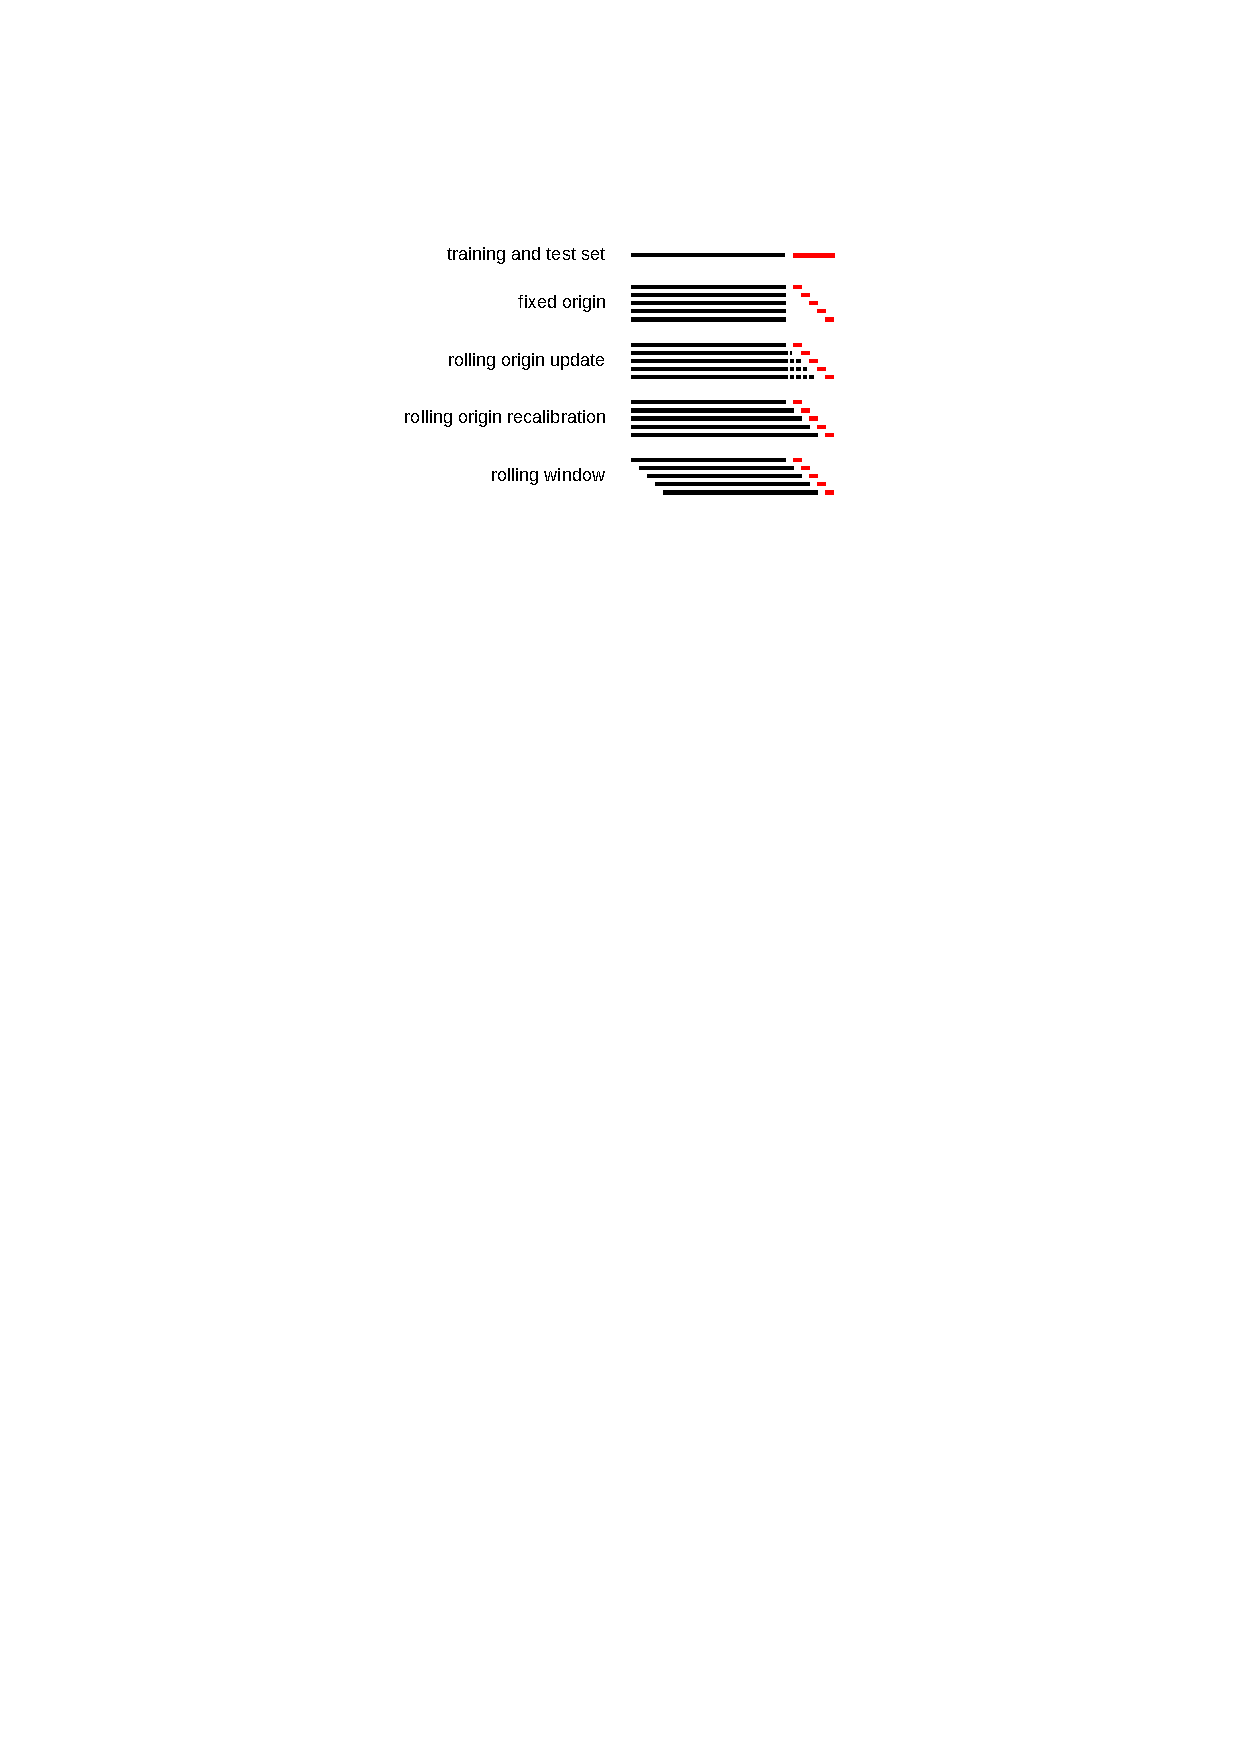
\includegraphics[width=0.6\textwidth]{figures/stats/rolling_forecast_origin}
\caption{
Illustration of multiple test train split methods for time series models \cite{bergmeir_dissertation}.
Note that $t$ is increasing along the $x$-axis.
In the fixed origin method, we do not do any retraining and the prediction quality
can be expected to drop as we go further into the future.
In the rolling origin update method, we do not retrain the model parameters $\vb*{\beta}$
with each iteration, but do update the $y_{i}$ lags.
In the rolling origin recalibration method we fully retrain the model on each iteration.
Lastly, in the rolling window method we remove data from the beginning of the training period
as we iterate to keep the training set a constant size.
This can help with some statistical interpretations of the model,
but also helps when working with slowly changing non-stationary data.
}
\label{fig:rolling_forecast_origin}
\end{figure}

Regardless of the test train split method, we can get a sense of the model's performance
qualitatively by looking at residual plots of $y_{t} - \yhat_{t}$.
The residuals will show any remaining systematic trends that the model did not learn,
as ideally they would be white noise.
Quantitatively, we can test
if the residuals are white noise with the Ljung--Box test of \cref{time_series:ljung_box},
as well as can compute the
root mean squared error\footnote{Also known as the root mean squared deviation (RMSD).} (RMSE)
and mean absolute percent error (MAPE)
between the predictions and observed values:

\begin{subequations}\label{eq:time_series:RMSE_MAPE}
\begin{align}
\text{RMSE}\left(\yhat\right) &= \sqrt{\expval{\left(y - \yhat\right)^{2}}} = \sqrt{\frac{1}{n}\sum_{t=1}^{n} \left(y_{t} - \yhat_{t}\right)^{2}}, \label{eq:time_series:RMSE} \\
\text{MAPE}\left(\yhat\right) &= \frac{\SI{100}{\percent}}{n} \sum_{t=1}^{n} \abs{\frac{y_{t} - \yhat_{t}}{y_{t}}}, \label{eq:time_series:MAPE} \\
\text{sMAPE}\left(\yhat\right) &= \frac{\SI{100}{\percent}}{n} \sum_{t=1}^{n} \frac{\abs{y_{t} - \yhat_{t}}}{\left(\abs{y_{t}} + \abs{\yhat_{t}}\right)/2}\,. \label{eq:time_series:sMAPE}
\end{align}
\end{subequations}

The symmetric mean absolute percent error (sMAPE)
\cref{eq:time_series:sMAPE} is an improvement on MAPE,
bounding values between \SI{0}{\percent} and \SI{200}{\percent}\footnote{Or
a more interpretable \SI{100}{\percent} if the factor of $2$ is omitted, as is common practice.}.
Note that $\text{sMAPE}\left(\yhat - \epsilon \right) \neq \text{sMAPE}\left(\yhat + \epsilon \right)$,
as symmetric here refers to sMAPE having an upper and lower bound.
This is in contrast to MAPE which is
bound at \SI{100}{\percent} for underestimates, $\yhat = y - \epsilon$\footnote{Assuming
$0 \leq y$ as is the case in many applications.}, but
unbound for overestimates, $\yhat = y + \epsilon$,
thereby tending to favor models that underestimate $y$.
Lastly, MAPE and sMAPE are both poorly behaved metrics if $y_{i} \simeq 0$.

%%%%%%%%%%%%%%%%%%%%%%%%%%%%%%%%%%%%%%%%%%%%%%%%%%%%%%%%
%%%%%%%%%%%%%%%%%%%%%%%%%%%%%%%%%%%%%%%%%%%%%%%%%%%%%%%%
\section{Box--Jenkins Method (Expanded)}
\label{time_series:box_jenkins}

The Box--Jenkins method, popularized in their book \cite{boxjen76},
is a recipe for fitting an ARMA-based model to a given time series $y_{t}$.
The steps have been expanded here to make the entire process
for working with time series data more explicit:

\begin{enumerate}[noitemsep]
  \item Do any necessary pre-cleaning of $y_{t}$ to normalize the data.\label{item:time_series:box_jenkins:cleaning0}
  \begin{enumerate}[noitemsep]
    \item \Zscore normalization, deterministic transforms $f\left(t\right)$, \etc.\label{item:time_series:box_jenkins:cleaning0:detail}
    \item Also, split the training and test sets.\label{item:time_series:box_jenkins:cleaning0:train_test_split}
  \end{enumerate}
  \item Check the stationarity and seasonality of the cleaned $y_{t}$.\label{item:time_series:box_jenkins:assumptions}
  \begin{enumerate}[noitemsep]
    \item Look at $y_{t}$ and the MA plot for obvious problems.\label{item:time_series:box_jenkins:assumptions:eye}
    \item Use the augmented Dickey--Fuller test (ADF) for stationary.\label{item:time_series:box_jenkins:assumptions:ADF}
    \item Correct any remaining problems with a ARIMA, $1 \leq d$, or SARIMA model.\label{item:time_series:box_jenkins:assumptions:cleaning1}
  \end{enumerate}
  \item Select the appropriate ARMA model, \ie choose $p$ and $q$.\label{item:time_series:box_jenkins:order}
  \begin{enumerate}[noitemsep]
    \item The PACF plot gives clues to the $\text{AR}\left(p\right)$ order.\label{item:time_series:box_jenkins:order:PACF}
    \item The ACF plot gives clues to the $\text{MA}\left(q\right)$ order.\label{item:time_series:box_jenkins:order:ACF}
  \end{enumerate}
  \item Fit the chosen model.\label{item:time_series:box_jenkins:fit}
  \item Verify the fitted model by checking the residuals. Return to \cref{item:time_series:box_jenkins:cleaning0} if needed.\label{item:time_series:box_jenkins:verify}
  \begin{enumerate}[noitemsep]
    \item Use the Ljung--Box test for white noise on the residuals.\label{item:time_series:box_jenkins:verify:Ljung_Box}
    \item Measure performance with RMSE and MAPE.\label{item:time_series:box_jenkins:verify:RMSE_MAPE}
    \item Measure the relative performance of multiple models with AIC and BIC.\label{item:time_series:box_jenkins:verify:AIC_BIC}
  \end{enumerate}
  \item Invert any cleaning steps to return to the original units of $y_{t}$ for predictions.\label{item:time_series:box_jenkins:invert}
\end{enumerate}

In \cref{item:time_series:box_jenkins:order} a simple approach is to
go out to the last significant non-zero order of $p$ ($q$) in the PACF (ACF) plot.
However, interpreting the PACF and ACF plots is a developed skill
and there are many different pieces of advice
available\footnote{See
\href{https://people.duke.edu/~rnau/411arim3.htm}{here}
and the Box--Jenkins method
\href{https://en.wikipedia.org/wiki/Box\%E2\%80\%93Jenkins\_method\#Autocorrelation\_and\_partial\_autocorrelation\_plots}{wikipedia page}
for just two examples.}.

%%%%%%%%%%%%%%%%%%%%%%%%%%%%%%%%%%%%%%%%%%%%%%%%%%%%%%%%
%%%%%%%%%%%%%%%%%%%%%%%%%%%%%%%%%%%%%%%%%%%%%%%%%%%%%%%%
\section{Auto-ARIMA}
\label{time_series:auto_ARIMA}
% TODO

%%%%%%%%%%%%%%%%%%%%%%%%%%%%%%%%%%%%%%%%%%%%%%%%%%%%%%%%
%%%%%%%%%%%%%%%%%%%%%%%%%%%%%%%%%%%%%%%%%%%%%%%%%%%%%%%%
\section{Unit Roots}
\label{time_series:unit_root}

A time series with $\abs{\phi} = 1$ for the leading AR coefficient
is said to have a unit root and is non-stationary.
More formally, we can construct the characteristic
equation\footnote{As if we were solving a
homogeneous linear ordinary differential equation with constant coefficients.} \cref{eq:time_series:unit_roots:characteristic}
for a $\text{AR}\left(p\right)$ time series $y_{t}$ and look for roots $m$.
If $m=1$ is one of the roots, the time series then has a unit root.

\begin{subequations}\label{eq:time_series:unit_roots}
\begin{gather}
y_{t} = \sum_{i=1}^{p} \phi_{i}\, y_{t-i} + \epsilon_{t}\,, \label{eq:time_series:unit_roots:y} \\
\implies m^{p} - \left(\, \sum_{i=1}^{p} \phi_{i}\, m^{i-1} \right) = 0. \label{eq:time_series:unit_roots:characteristic}
\end{gather}
\end{subequations}

Time series with unit roots are non-stationary,
as can be illustrated with the $\text{AR}\left(1\right)$ series\footnote{The expansion
in \cref{eq:time_series:unit_root_ex:expand} is really
$\text{AR}\left(1\right) = \text{MA}\left(\infty\right)$ \cref{eq:time_series:invert:AR_1} written out.}:

\begin{subequations}\label{eq:time_series:unit_root_ex}
\begin{align}
y_{t}
= \phi\, y_{t-1} + \epsilon_{t}
&= \phi \left(\phi\, y_{t-2} + \epsilon_{t-1}\right) + \epsilon_{t}
= \cdots
= \phi^{t} y_{0} + \sum_{i=0}^{t-1} \phi^{i} \epsilon_{t-i}\,, \label{eq:time_series:unit_root_ex:expand} \\
\expval{y_{t}}
&= \phi^{t} \expval{y_{0}} + \sum_{i=0}^{t-1} \phi^{i} \expval{\epsilon_{t-i}}
= \phi^{t} y_{0}\,, \label{eq:time_series:unit_root_ex:expval} \\
\variance{y_{t}}
&= \phi^{2t}\, \variance{y_{0}} + \sum_{i=0}^{t-1} \phi^{2i}\, \variance{\epsilon_{t-i}}
= \sigma^{2} \sum_{i=0}^{t-1} \phi^{2i}. \label{eq:time_series:unit_root_ex:var}
\end{align}
\end{subequations}

\noindent Note that we are assuming the errors only contain white noise,
and thus are uncorrelated with constant variance $\variance{\epsilon} = \sigma^{2}$.
When $\abs{\phi} < 1$, $\expval{y_{t}} \to 0$ and
$\variance{y_{t}} \to \sigma^{2}/\left(1-\phi^{2}\right)$ are constant
as $t \to \infty$, and the time series is stationary.
When $1 < \abs{\phi}$, $\expval{y_{t}} = \phi^{t} y_{0}$
will diverge as $t \to \infty$, and the time series is clearly non-stationary\footnote{Technically,
the time series is an ``explosive process'', more than just non-stationary.}.
When we have a unit root $\abs{\phi} = 1$,
$\expval{y_{t}} = y_{0}$ is constant\footnote{Making these unit roots harder to identify visually.},
but $\variance{y_{t}} = t \sigma^{2}$ is not constant and the time series is non-stationary.

Lastly, a time series with unit roots can be made stationary through
differencing\footnote{$d_{t} \equiv y_{t} - y_{t-1} = \epsilon_{t}$, $\expval{d_{t}} = 0$, $\variance{d_{t}} = \sigma^{2}$.}.
In particular, if the $m=1$ unit root of the characteristic equation has multiplicity $d$,
a $\text{I}\left(d\right)$ model will make the time series stationary.

%%%%%%%%%%%%%%%%%%%%%%%%%%%%%%%%%%%%%%%%%%%%%%%%%%%%%%%%
%%%%%%%%%%%%%%%%%%%%%%%%%%%%%%%%%%%%%%%%%%%%%%%%%%%%%%%%
\section{Augmented Dickey--Fuller (ADF) Test for Stationarity}
\label{time_series:ADF}

The augmented\footnote{The ADF is an extension of the normal Dickey--Fuller test where $p = 1$.} Dickey--Fuller (ADF) test
is a hypothesis tests for the stationarity of a time series.
We begin by assuming the time series for $y$ is a $\text{AR}\left(p\right)$ model \cref{eq:time_series:AR}
and construct the difference:

\begin{subequations}\label{eq:time_series:ADF}
\begin{align}
\Delta y_{t} &= y_{t} - y_{t-1} = \phi_{0} + \delta y_{t-1} + \sum_{i=2}^{p} \phi_{i}\, y_{t-i} + \epsilon_{t}, \label{eq:time_series:ADF:Delta_y} \\
\delta &= \phi_{1} - 1. \label{eq:time_series:ADF:delta}
\end{align}
\end{subequations}

Now we test $H_{0}$ that $0 \leq \delta$ and the time series is
non-stationary\footnote{As $\delta = 0 \implies \phi_{1} = 1$,
\ie the time series has a unit root and is non-stationary.
Note that it is possible to have a non-stationary time series without a unit root,
thus the ADF test is not fully comprehensive.} versus
the alternative hypothesis $H_{a}$ that $\delta < 0$, \ie time series is stationary.
We fit the data and then perform the hypothesis testing with test statistic
$t_{\hat{\delta}} = \hat{\delta} / \text{Standard Error}\left(\hat{\delta}\right)$
by comparing to the Dickey--Fuller distribution\footnote{We can not use the standard \tdist as $y_{t-1}$ is still assumed to be non-stationary under $H_{0}$.}.
If we can reject $H_{0}$ we therefore have shown that $y_{t}$ is stationary.
Note we can further extend the ADF test by replacing the constant $\phi_{0}$
with a deterministic, quadratic, time trend $\phi_{0} + a_{1} t + a_{2} t^{2}$.
The ADF test is available via the \texttt{adfuller}
\href{https://www.statsmodels.org/stable/generated/statsmodels.tsa.stattools.adfuller.html}{function}.

%%%%%%%%%%%%%%%%%%%%%%%%%%%%%%%%%%%%%%%%%%%%%%%%%%%%%%%%
%%%%%%%%%%%%%%%%%%%%%%%%%%%%%%%%%%%%%%%%%%%%%%%%%%%%%%%%
\section{Ljung--Box Test for White Noise}
\label{time_series:ljung_box}

The Ljung--Box test tests if a time series $y$ solely consists of white noise
by looking at multiple lags of the ACF.
The test statistic is

\begin{equation}\label{eq:time_series:ljung_box:Q}
Q = n \left(n+2\right) \sum_{i=1}^{h} \frac{\corr{y_{t}}{y_{t-i}}^{2}}{n-i}
\end{equation}

\noindent where $n$ is the sample size and $h$ is the number of lags to be tested.
Using the \chiSqdist with $\nu = h$ degrees of freedom we find the critical $Q_{c}$
and reject $H_{0}$, the data is white noise, if $Q_{c} < Q$.
If we fail to reject $H_{0}$, \ie $Q \leq Q_{c}$, we have shown $y$ is white noise.
Note that if we are performing the Ljung--Box test on the remainders of a fitted model, such as $\text{ARIMA}\left(p,d,q\right)$,
we must adjust the degrees of freedom accordingly, $\nu = h - p - d - q$.
The Ljung--Box test can be performed with the \texttt{acorr\_ljungbox}
\href{https://www.statsmodels.org/stable/generated/statsmodels.stats.diagnostic.acorr_ljungbox.html}{function}.

%%%%%%%%%%%%%%%%%%%%%%%%%%%%%%%%%%%%%%%%%%%%%%%%%%%%%%%%
%%%%%%%%%%%%%%%%%%%%%%%%%%%%%%%%%%%%%%%%%%%%%%%%%%%%%%%%
\section{Granger Causality}
\label{time_series:granger_causality}

When one time series, $x_{t}$, appears to
predict the behavior of another time series, $y_{t}$,
we can test for Granger causality \cite{10.2307/1912791}.
We begin by constructing two $\text{AR}\left(p\right)$ models:

\begin{subequations}\label{eq:time_series:granger_causality}
\begin{align}
\text{AR}_{y}\left(p_{y}\right) &= \phi_{y}\left(L,p_{y}\right) y_{t} + \epsilon_{t}\,, \label{eq:time_series:granger_causality:y} \\
\text{AR}_{y,x}\left(p_{y}, p_{x}\right) &= \phi_{y}\left(L,p_{y}\right) y_{t} + \phi_{x}\left(L,p_{x}\right) x_{t} + \epsilon_{t}\,, \label{eq:time_series:granger_causality:yx}
\end{align}
\end{subequations}

\noindent where $\text{AR}_{y}$ is only a function of the $y_{t}$ time series,
and $\text{AR}_{y,x}$ is a function of both the $y_{t}$ and $x_{t}$ time series.
For both models we test the $\phi$ coefficients for significance\footnote{The
individual coefficient significances are determined via \ttest methods,
while a \Ftest of lack-of-fit sum of squares, \cref{regression:goodness_of_fit:F_test_fit},
is used to test the model fit as a whole.} individually,
removing any non-significant lags, and collectively for the whole model.
After this process, if $\text{AR}_{y,x}$ still contains $x_{t}$ terms
and is found to fit $y$ better than $\text{AR}_{y}$,
we can say that $x_{t}$ Granger-causes $y_{t}$.
More formally, the null hypothesis $H_{0}$ that $x_{t}$ does not Granger-cause $y_{t}$,
is accepted if and only if all $\phi_{x}$ terms have been removed from the final model.

A confirmation of Granger causality does not imply ``true causality'' in the general sense,
it is merely a statement that a linear model of $x_{t}$ forecasts, or predicts, $y_{t}$.
For example, there maybe latent confounding effects behind both $x_{t}$ and $y_{t}$
which would require a more sophisticated analysis to detect or rule out.
Even with this limited causal interpretation,
there are still challenges \cite{GRASSMANN2020} to the validity of Granger causality.

%%%%%%%%%%%%%%%%%%%%%%%%%%%%%%%%%%%%%%%%%%%%%%%%%%%%%%%%
%%%%%%%%%%%%%%%%%%%%%%%%%%%%%%%%%%%%%%%%%%%%%%%%%%%%%%%%
\section{Bayesian Approaches}
\label{time_series:bayesian_approaches}

We can also look at time series analysis within a Bayesian framework;
assuming prior distributions for the model parameters $\vb*{\beta}$
then updating based on the observed data,
thereby producing distributions of our predictions and parameters instead of only MLE point estimates.
The \pymcThree \href{https://docs.pymc.io}{module}
has \href{https://docs.pymc.io/api/distributions/timeseries.html}{timeseries functions}
for implementing this approach, including AR and GARCH models.

%%%%%%%%%%%%%%%%%%%%%%%%%%%%%%%%%%%%%%%%%%%%%%%%%%%%%%%%
%%%%%%%%%%%%%%%%%%%%%%%%%%%%%%%%%%%%%%%%%%%%%%%%%%%%%%%%
\section{Prophet}
\label{time_series:prophet}
% TODO Probably add greykite as well

%%%%%%%%%%%%%%%%%%%%%%%%%%%%%%%%%%%%%%%%%%%%%%%%%%%%%%%%
%%%%%%%%%%%%%%%%%%%%%%%%%%%%%%%%%%%%%%%%%%%%%%%%%%%%%%%%
\section{Anomaly Detection}
\label{time_series:anomaly_detection}

% TODO
% https://youtu.be/XPwCo4cqqt0

%%%%%%%%%%%%%%%%%%%%%%%%%%%%%%%%%%%%%%%%%%%%%%%%%%%%%%%%
%%%%%%%%%%%%%%%%%%%%%%%%%%%%%%%%%%%%%%%%%%%%%%%%%%%%%%%%
\section{Kalman Filters}
\label{time_series:kalman_filters}
% TODO
}
%%%%%%%%%%%%%%%%%%%%%%%%%%%%%%%%%%%%%%%%%%%%%%%%%%%%%%%%
%%%%%%%%%%%%%%%%%%%%%%%%%%%%%%%%%%%%%%%%%%%%%%%%%%%%%%%%
\section{Survival Analysis}
\label{additional:Survival}

Survival analysis is a subfield of statistics which examines problems involving the timing of events
such as death, component failure, or exiting a line of therapy after an adverse effect, in a population of subjects under study.
Using the appropriate models, quantities such as the lifetime, or failure rate, of a subject
can be estimated, as well as their dependence on other independent variables.
A variety of common models are available,
each with their own assumptions, capabilities, and limitations,
which make them best suited for certain applications.

%%%%%%%%%%%%%%%%%%%%%%%%%%%%%%%%%%%%%%%%%%%%%%%%%%%%%%%%
\subsection{Nomenclature}
\label{additional:Survival:Nomenclature}

\begin{symbollist}
	\item[Event] The event of interest in a study, \eg death, component failure\ldots
	\item[$t$] Time from the start of observation to an event, the conclusion of the study, or the withdrawal of a subject.
	\item[$T$] Time that an event occurred.
	\item[$x$] Independent variable(s) under consideration.
	\item[Censoring] Right\footnote{Left censored subjects enter the study after the event of interest has already occurred at an unknown $t < 0$.} censored subjects have no events during the observation period, either due to early withdrawal or the conclusion of the study. The true lifetime of these subjects is unavailable for analysis, \ie they have been censored.
	\item[$S\left(t\right)$] The survival function $S\left(t\right)$ is the probability that a subject survives longer than $t$, \ie $S\left(t\right) = P\left(T > t\right)$.
	\item[$F\left(t\right)$] The lifetime distribution function $F\left(t\right)$ is the complement of the survival function, \ie $F\left(t\right) = 1 - S\left(t\right) = P\left(T \leq t\right)$.
	\item[$f\left(t\right)$] The event density function $f\left(t\right)$ is the time derivative of the lifetime distribution function $F\left(t\right)$, $f\left(t\right) = \frac{dF}{dt} = -\frac{dS}{dt}$, if it exists.
	\item[$\lambda\left(t\right)$] The hazard function $\lambda\left(t\right)$ is the event rate at $t$ conditional on survival to time $t$, \ie $T > t$, see \cref{eq:Survival:hazard_def}. Any $\lambda\left(t\right)$ can be a hazard function, provided it satisfies \cref{eq:Survival:hazard_cond}.
	\item[$\Lambda\left(t\right)$] The cumulative hazard function $\Lambda\left(t\right)$ is the integral of $\lambda\left(t\right)$ with respect to time \cref{eq:Survival:cum_hazard:def}. Also see the relations in \cref{eq:Survival:cum_hazard:to_lambda,eq:Survival:cum_hazard:to_S}.
	\item[HR] The hazard ratio (HR) compares the hazards of two subsets of subjects partitioned by $x$ at time $t$, $\text{HR} = \lambda\left(x = 1\right) / \lambda\left(x=0\right)$.
\end{symbollist}

\begin{subequations}\label{eq:Survival:hazard_def}
\begin{align}
\lambda\left(t\right) dt &= P\left(T \leq t + dt \mid T > t\right),\,\text{as} \,\, dt \to 0 \label{eq:Survival:hazard_def:a} \\
\lambda\left(t\right) &= \lim_{dt \to 0} \frac{P\left(T \leq t + dt \cap T > t\right)}{P\left(T > t\right)\,dt} \label{eq:Survival:hazard_def:b} \\
&= \frac{1}{S\left(t\right)} \lim_{dt \to 0} \frac{P\left(t < T \leq t + dt\right)}{dt} \label{eq:Survival:hazard_def:c} \\
&= \frac{1}{S\left(t\right)} \lim_{dt \to 0} \frac{F\left(t + dt\right) - F\left(t\right)}{dt} \label{eq:Survival:hazard_def:d} \\
&= \frac{f\left(t\right)}{S\left(t\right)} = -\frac{1}{S} \frac{dS}{dt} \label{eq:Survival:hazard_def:e}
\end{align}
\end{subequations}

\begin{subequations}\label{eq:Survival:hazard_cond}
\begin{gather}
\forall t \geq 0, \, \lambda\left(t\right) \geq 0 \label{eq:Survival:hazard_cond:a} \\
\int_{0}^{\infty} \lambda\left(t\right) \, \dif t = \infty \label{eq:Survival:hazard_cond:b}
\end{gather}
\end{subequations}

\begin{subequations}\label{eq:Survival:cum_hazard}
\begin{gather}
\Lambda\left(t\right) = \int_{0}^{t} \lambda\left(u\right) \, \dif u = - \ln\left(S\left(t\right)\right) \label{eq:Survival:cum_hazard:def} \\
\lambda\left(t\right) = \frac{d\Lambda}{dt} = -\frac{1}{S} \frac{dS}{dt} \label{eq:Survival:cum_hazard:to_lambda} \\
S\left(t\right) = \exp\left(-\Lambda\left(t\right)\right) \label{eq:Survival:cum_hazard:to_S}
\end{gather}
\end{subequations}

%%%%%%%%%%%%%%%%%%%%%%%%%%%%%%%%%%%%%%%%%%%%%%%%%%%%%%%%
\subsection{Kaplan-Meier Model}
\label{additional:Survival:km}

The Kaplan-Meier model \cite{km} $\hat{S}_{\text{KM}}\left(t\right)$ is a non-parametric
estimate of $S\left(t\right)$ computed from empirical data.

\begin{equation}\label{eq:Survival:km}
\hat{S}_{\text{KM}}\left(t\right) = \prod_{i:\,t_{i} < t} \left(1 - \frac{d_{i}}{n_{i}}\right)
\end{equation}

\noindent Here the product is over all times $t_{i}$ at which $d_{i}$ events occurred,
and $n_{i}$ is the number of subjects still under study at $t_{i}$,
\ie subjects who have not had an event or been censured.
Due to its construction, $\hat{S}_{\text{KM}}\left(t\right)$ remains steady
between $t_{i}$ but drops vertically at each data point.
Therefore the derivative does not exist and we can not estimate $f\left(t\right)$ or $\lambda\left(t\right)$.
See \cref{fig:stanford_km:km} for one example of a Kaplan-Meier curve.

We can apply the Kaplan-Meier estimator to different subsets of subjects partitioned by a categorical variable $x$
in order to understand the dependence of $S\left(t\right)$ on $x$.
Note that $x$ can not be a continuous variable, and must be binned to integer classes if that is the case.

%%%%%%%%%%%%%%%%%%%%%%%%%%%%%%%%%%%%%%%%%%%%%%%%%%%%%%%%
\subsection{Exponential Model}
\label{additional:Survival:exp}

The exponential model is a parametric estimate of $S\left(t\right)$
valid when the hazard is expected to be constant with respect to $t$.
In nuclear physics\footnote{$\frac{dN}{dt} = -\lambda N$, $N\left(t\right) = N_{0} e^{-\lambda t}$, half-life $t_{1/2} = \ln\left(2\right) / \lambda = \tau \ln\left(2\right)$, where $\tau$ is the time constant.} $\lambda\left(t\right) = \lambda$
decays per unit time really is a constant.
However, in most situations $\lambda = c$ is unrealistic over longer time scales,
as illustrated in \cref{additional:Survival:additional:bathtub}.
The exponential model can accommodate both categorical and continuous $x$ independent variables.

The survival function for the exponential model is simply

\begin{equation}\label{eq:Survival:exp}
\hat{S}_{\text{Exp}}\left(t\right) = e^{-\lambda t}
\end{equation}

\noindent where the hazard can be expanded in terms of $\mathbf{x}$, $\bm{\beta}$ as in a regression analysis:

\begin{equation}\label{eq:Survival:exp_lambda}
\begin{aligned}
\lambda\left(x\right) &= \exp\left(\beta_{0} + \sum_{j=1}^{n}\, \beta_{j} x_{j}\right) \\
\log\left(\lambda\right) &= \mathbf{x} \bm{\beta}
\end{aligned}
\end{equation}

\noindent Here we are making the {\em proportional hazards assumption},
\ie the differences in $\lambda$ between subgroups in $x_{j}$
are proportional\footnote{Really $\log\left(\lambda\right) \propto \beta$.} to $\beta_{j}$
and constant over $t$.
To find the best estimate of $\hat{\bm{\beta}}$,
$\lambda$ is used to derive a likelihood function which is
then optimized\footnote{The exact details of this optimization are handled by common software libraries and are omitted here. Similar approaches are also used to fit the later Weibull and Cox proportional-hazards models.}.

The hazard ratio for $x_{j}$ is:

\begin{equation}\label{eq:Survival:exp_HR}
\begin{aligned}
\text{HR}_{\text{Exp}} &= e^{\ldots+\beta_{j} 1+\ldots} / e^{\ldots+\beta_{j} 0+\ldots} \\
&= e^{\beta_{j}}
\end{aligned}
\end{equation}

\subsubsection{Weibull Model}
\label{additional:Survival:weibull}

The Weibull model expands on the standard exponential model
by introducing a shape parameter $k$ to adjust the time dependence of the hazard:

\begin{equation}\label{eq:Survival:weibull}
\begin{aligned}
\hat{S}_{\text{Weibull}}\left(t\right) &= e^{-\lambda_{\text{Weibull}} t} \\
\lambda_{\text{Weibull}} &= \exp\left(\beta_{0} t^{k} + \sum_{j=1}^{n}\, \beta_{j} x_{j}\right) \\
\text{HR}_{\text{Weibull}} &= e^{\beta_{j}}
\end{aligned}
\end{equation}

\noindent Here $\beta_{0}$ is the scale parameter of the hazard with respect to $t$,
while the other $\beta_{j}$ are scale parameters for the independent $x_{j}$.
For $k<0$ ($k>0$) the hazard monotonically decreases (increases) over time,
while $k=0$ returns the exponential model.
This allows phenomena such as burn in and compounding component failures to be modeled.
Numerous parameterizations and expansions of the Weibull model are available,
however they all share the property that
$\lambda = \exp\left(\beta_{0} f\left(t\right) + \sum_{j=1}^{n}\, \beta_{j} x_{j}\right)$
where $f\left(t\right)$ is a {\em known}, almost always monotonic, function of $t$.

%%%%%%%%%%%%%%%%%%%%%%%%%%%%%%%%%%%%%%%%%%%%%%%%%%%%%%%%
\subsection{Cox Proportional-Hazards Model}
\label{additional:Survival:cox}

The Cox proportional-hazards model \cite{cox} is a
semiparametric\footnote{Semiparametric as $\lambda_{0}\left(t\right)$ is unspecified, but $\bm{\beta}$ are still parameters of $\lambda$.} model
which further expands on the Weibull model by allowing
the time dependence of $\lambda$ to be an unknown function.
As the name suggests, the proportional hazards assumption is retained
allowing us to compute useful HR values
without even knowing $\lambda\left(t\right)$, or $S\left(t\right)$.

In the Cox model we assume the hazard has the form of

\begin{equation}\label{eq:Survival:cox_lambda}
\lambda_{\text{Cox}} = \lambda_{0}\left(t\right) \exp\left(\sum_{j=1}^{n}\, \beta_{j} x_{j}\right)
\end{equation}

\noindent where $\lambda_{0}\left(t\right)$ is the baseline hazard, an unspecified function of $t$.
When computing hazard ratios $\lambda_{0}\left(t\right)$ then drops out:

\begin{equation}\label{eq:Survival:cox_HR}
\text{HR}_{\text{Exp}} = e^{\beta_{j}}
\end{equation}

%%%%%%%%%%%%%%%%%%%%%%%%%%%%%%%%%%%%%%%%%%%%%%%%%%%%%%%%
\subsection{Method Comparison}
\label{additional:Survival:comp}

\begin{table}[H]
\centering
\begin{tabular}{l|l|l}
\multicolumn{1}{c|}{Kaplan-Meier} & \multicolumn{1}{c|}{Exponential / Weibull} & \multicolumn{1}{c}{Cox} \\
\cline{1-3}
\begin{tabular}[c]{p{0.3\textwidth}}
Pro
\begin{itemize}
	\item Simple to compute and understand
	\item Can estimate $S$
\end{itemize}
\\
Con
\begin{itemize}
	\item No functional form
	\item Can \textbf{not} estimate HR
	\item Only can handle a few categorical $x$
\end{itemize}
\end{tabular}

&

\begin{tabular}[c]{p{0.3\textwidth}}
Pro
\begin{itemize}
	\item Can estimate $S$ and HR
\end{itemize}
\\
Con
\begin{itemize}
	\item $\lambda\left(t\right) = c$ can be unrealistic
	\item Weibull: $\lambda = f\left(t\right)$ of a known form
\end{itemize}
\end{tabular}

&

\begin{tabular}[c]{p{0.3\textwidth}}
Pro
\begin{itemize}
	\item $\lambda$ can be an unknown function of $t$
	\item Can estimate HR
\end{itemize}
\\
Con
\begin{itemize}
	\item Can \textbf{not} estimate $S$
\end{itemize}
\end{tabular}

\\
\end{tabular}
\end{table}

%%%%%%%%%%%%%%%%%%%%%%%%%%%%%%%%%%%%%%%%%%%%%%%%%%%%%%%%
\subsection{Model Assumptions}
\label{additional:Survival:assumptions}

\begin{enumerate}[noitemsep]
\item Any censoring is non-informative, \ie censoring is uncorrelated with the probabilities of different event outcomes.\label{item:Survival:assumptions:censoring}
\item Survival times $t$ are uncorrelated across subjects.\label{item:Survival:assumptions:t_uncorr}
\item $\mathbf{x}$ is constant over time, per subject.\label{item:Survival:assumptions:X_constant}
\item Hazards are proportional, \ie hazard ratios are constant over time.\label{item:Survival:assumptions:prop_hazard}
\item $\log\left(\lambda\right)$ is linear with respect to the numerical $x_{j}$ independent variables.\label{item:Survival:assumptions:X_linearity}
\end{enumerate}

\cref{item:Survival:assumptions:censoring,item:Survival:assumptions:t_uncorr,item:Survival:assumptions:X_constant}
are assumptions for all survival models, while
\cref{item:Survival:assumptions:prop_hazard,item:Survival:assumptions:X_linearity}
apply to the exponential, Weibull and Cox models.

\subsubsection{Tests and Corrections}
\label{additional:Survival:assumptions:tests_and_corrections}

\begin{itemize}[noitemsep]
\item[\cref{item:Survival:assumptions:censoring}.] Exploratory data analysis to detect differences in $\mathbf{x}$ distributions between censored and non-censored subjects. If violated, better input data is needed, redesign study.

\item[\cref{item:Survival:assumptions:t_uncorr}.] Exploratory data analysis, study design question. If violated, redesign study.

\item[\cref{item:Survival:assumptions:X_constant}.] Exploratory data analysis, study design question. If unavoidable, can try a more complex time dependent covariate model.

\item[\cref{item:Survival:assumptions:prop_hazard}.] Check with a Schoenfeld test or complementary log-log plot. If violated, stratify problematic $x_{j}$ variables into separate models, or use more complex models with time dependent $\beta$ coefficients.

\item[\cref{item:Survival:assumptions:X_linearity}.] Check the appropriate residual plot. If violated, try to linearize the offending numerical $x_{j}$ with a transformation or bin to a categorical variable.
\end{itemize}

\subsubsection{Schoenfeld Test}
\label{additional:Survival:assumptions:schoenfeld}

Schoenfeld residuals are similar in concept to normal residuals in regression analyses,
but instead of looking at the difference between the true and estimated values of $y$,
$\hat{\bm{\epsilon}} = \mathbf{y} - \mathbf{X} \hat{\bm{\beta}}$,
we look at the difference in $\bm{\beta}$ and $\hat{\bm{\beta}}$ for a particular $y$ value.
In this way, Schoenfeld residuals represent the difference in the
coefficient $\beta_{j}$ fit from all data points, and a single point.
To validate the proportional hazards assumption
the Schoenfeld residuals \cite{schoenfeld} must not change over time.
An example Schoenfeld residual plot is provided in
\cref{fig:cox:schoenfeld_residuals}.
Besides graphically looking at the residuals,
we can use $\chi^{2}$-tests to compute {\pvalue}s
to test the null hypothesis, \ie the Schoenfeld residuals and time are independent.
In this case, the proportional hazards assumption is supported
if we find large, non-significant {\pvalue}s.

\subsubsection{Complementary Log-Log Plot}
\label{additional:Survival:assumptions:cloglog}

For categorical variables we can look at the
complementary log-log plot
of $\log\left(-\log\left(S\left(t\right)\right)\right)$ versus $\log\left(t\right)$.
An example complementary log-log plot is provided in \cref{fig:stanford_cloglog}.
If the different categories have parallel curves
the proportional hazards assumption is
valid for the variable in question.

%%%%%%%%%%%%%%%%%%%%%%%%%%%%%%%%%%%%%%%%%%%%%%%%%%%%%%%%
\subsection{Additional Concepts}
\label{additional:Survival:additional}

\subsubsection{Logrank Test}
\label{additional:Survival:additional:logrank}
% TODO comparing survival curves

\subsubsection{$G^{\rho}$ Test (survdiff)}
\label{additional:Survival:additional:survdiff}
% TODO comparing survival curves
TODO \texttt{survdiff}

\subsubsection{Concordance Statistic}
\label{additional:Survival:additional:concordance}
% TODO

\subsubsection{Relative Risk}
\label{additional:Survival:additional:RR}
% TODO relationship / differences from HR

\subsubsection{Odds Ratio}
\label{additional:Survival:additional:OR}
% TODO relationship / differences from HR

\subsubsection{Expected Future Lifetime}
\label{additional:Survival::additional:efl}

The expected future lifetime $\expval{T-t_{0}}$ is the
expected additional time of survival for a subject having already survived to $t_{0}$.
We can derive $\expval{T-t_{0}}$ \cref{eq:Survival:efl_der:efl}
from the probability of an event occurring between $t_{0}$ and $t_{0} + t$ \cref{eq:Survival:efl_der:P}
using the prior work of \cref{eq:Survival:hazard_def} and integration by parts:

\begin{subequations}\label{eq:Survival:efl_der}
\begin{gather}
P\left(T \leq t_{0} + t \mid T > t_{0}\right)
= \frac{F\left(t_{0} + t\right) - F\left(t_{0}\right)}{S\left(t_{0}\right)} \label{eq:Survival:efl_der:P} \\
\text{PDF}
= \frac{d}{dt} P\left(T \leq t_{0} + t \mid T > t_{0}\right)
= \frac{f\left(t_{0} + t\right)}{S\left(t_{0}\right)} \label{eq:Survival:efl_der:pdf} \\
\expval{T-t_{0}}
= \int_{0}^{\infty} t \, \text{PDF} \, \dif t
= \frac{1}{S\left(t_{0}\right)} \int_{0}^{\infty} S\left(t\right) \, \dif t \label{eq:Survival:efl_der:efl}
\end{gather}
\end{subequations}

\subsubsection{Bathtub Curve}
\label{additional:Survival:additional:bathtub}

In reliability engineering the hazard function of many components
can be estimated as a three part ``bathtub'' curve.
Initially the failure, \ie event, rate decreases as defective components fail early,
before reaching a constant plateau where failures are essentially random events.
As components wear out and reach the end of their useful lifetimes, the failure rate increases again.
Combining these three effects produces a bathtub-shaped curve, as seen in \cref{fig:bathtub_curve}.
We can model these situations with the Cox proportional-hazards model,
or a Weibull model with an appropriately shaped $\lambda\left(t\right)$.

\begin{figure}[H]
\centering
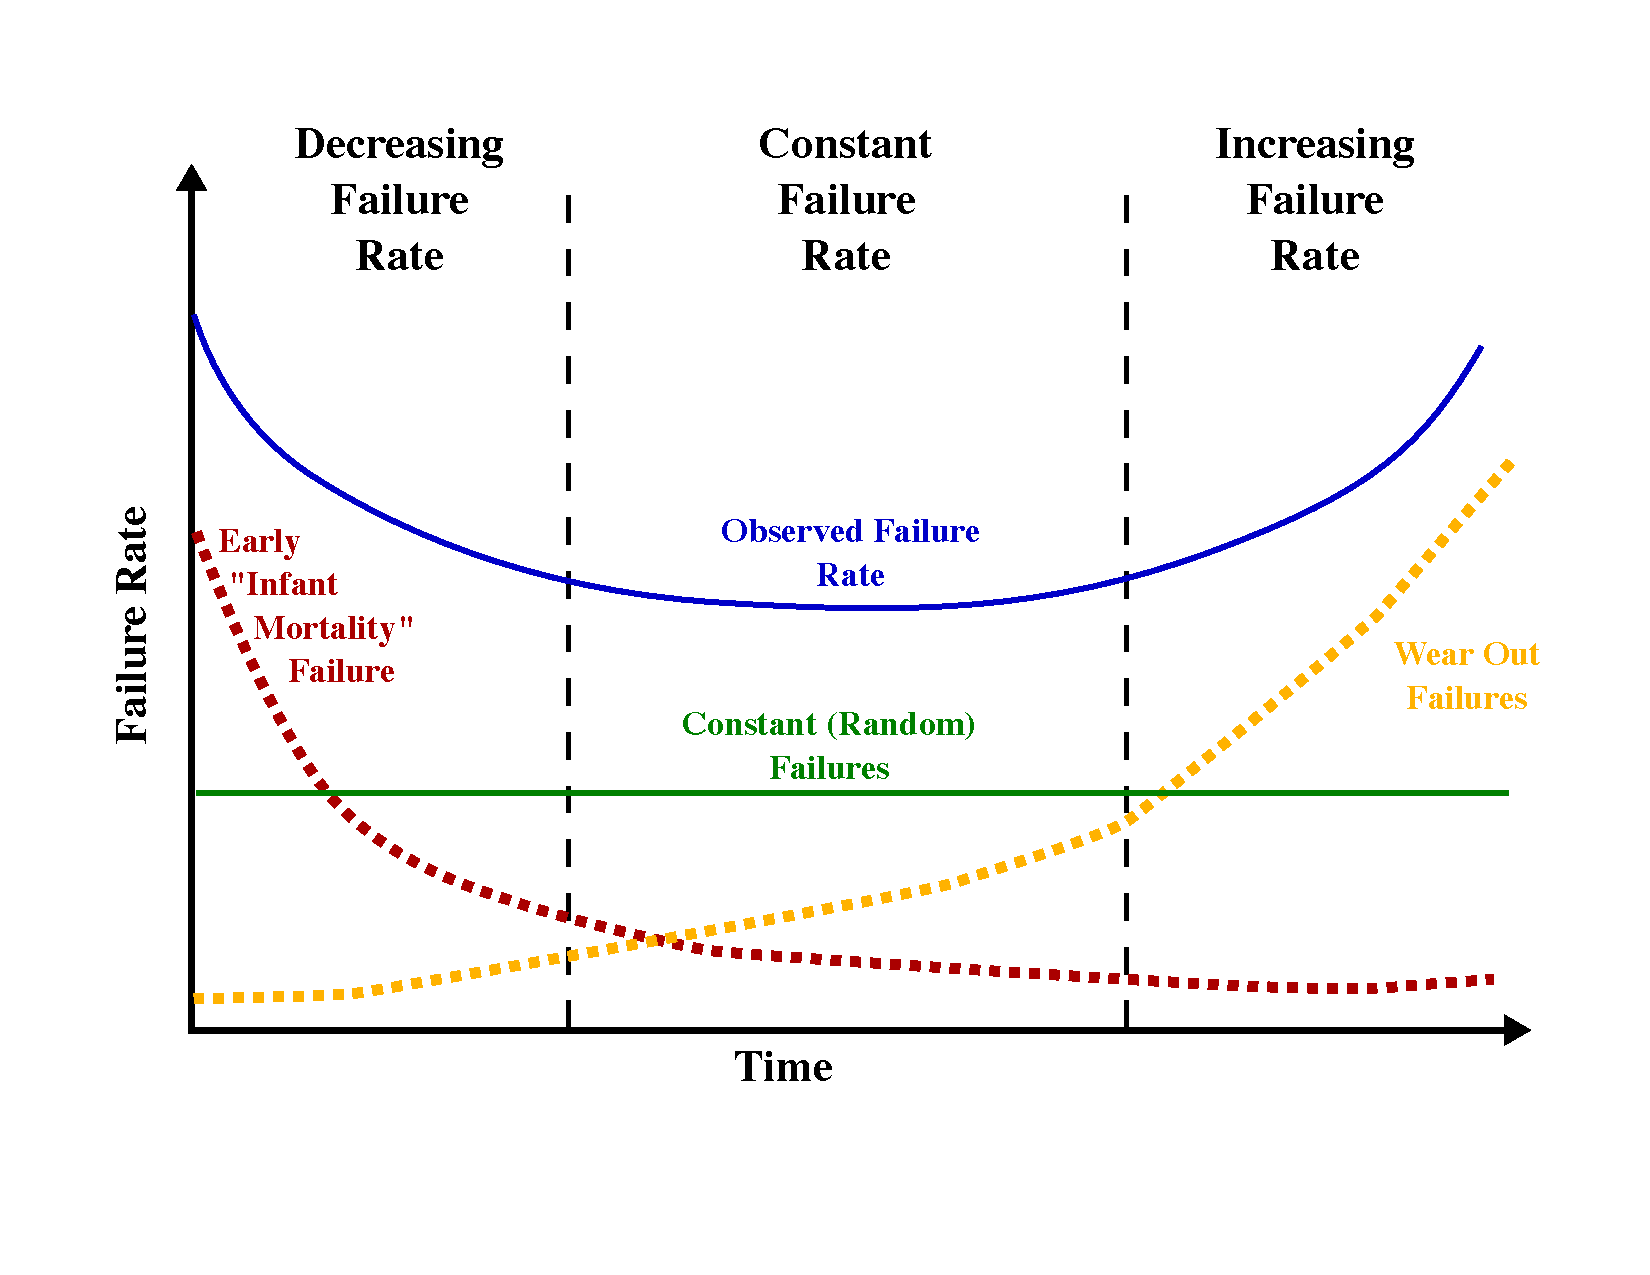
\includegraphics[width=0.7\textwidth]{figures/survival/bathtub_curve}
\vspace{0.2cm}
\caption{
Illustration of a bathtub curve hazard function, by \href{https://en.wikipedia.org/wiki/File:Bathtub_curve.svg}{Wyatts}.
}
\label{fig:bathtub_curve}
\end{figure}

%%%%%%%%%%%%%%%%%%%%%%%%%%%%%%%%%%%%%%%%%%%%%%%%%%%%%%%%
\subsection{Example \R Code}
\label{additional:Survival:Rcode}

% TODO link to code section from body section(s)

A simple example survival analysis in \R utilizing the built-in
\texttt{stanford2} Stanford heart transplant dataset is provided in this section.
The full code can also be found in
\href{https://github.com/mepland/data_science_notes/blob/main/sections/appendixes/additional/example_survival.R}{\texttt{example\_survival.R}}.
The status variable represents the event, death of a patient, as $\text{status}=1$,
and the censoring of a patient as $\text{status}=0$.
Three independent variables $x$ are available,
age in years,
age categories - under or over 40,
and the numeric T5 mismatch score between donor and recipient.

\begin{figure}[H]
\centering
  \begin{subfigure}[c]{0.48\textwidth}\centering
  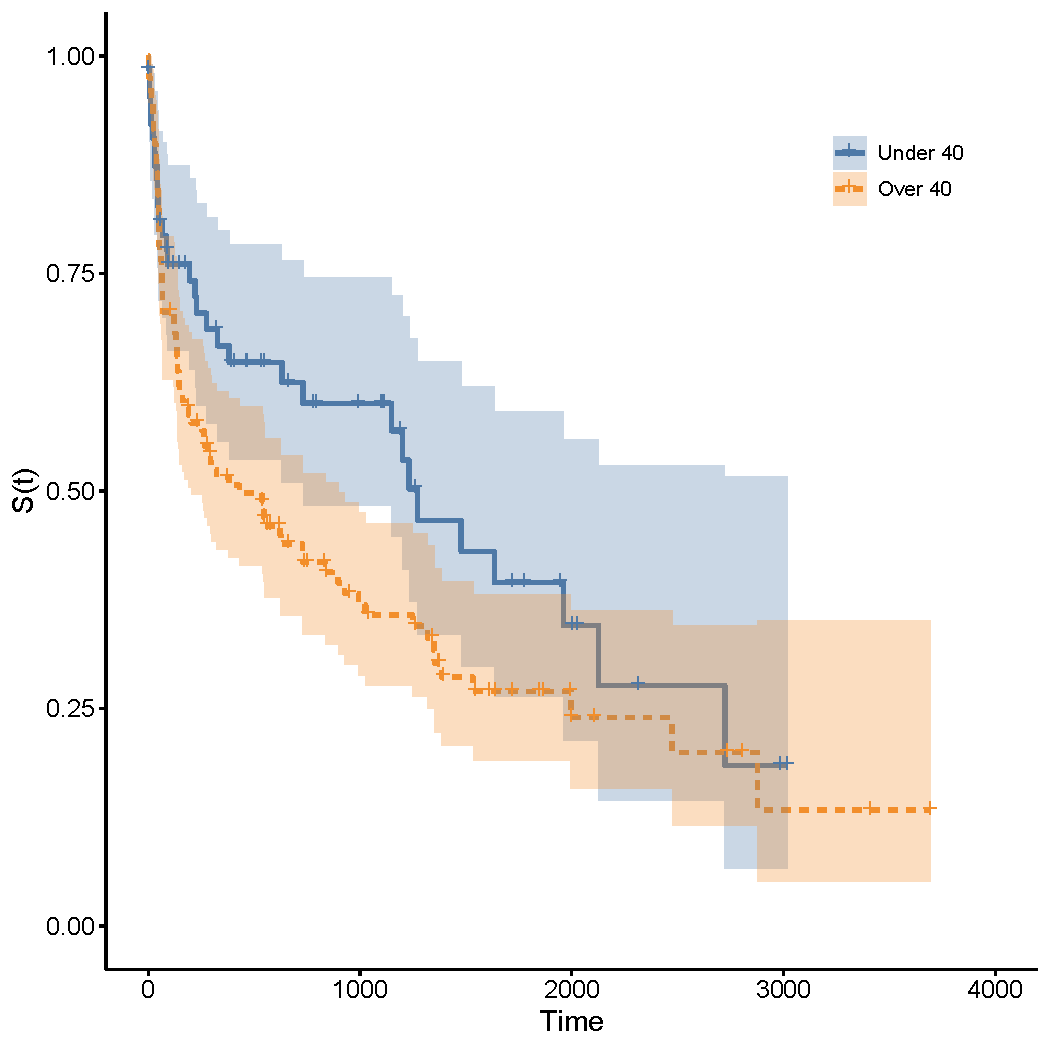
\includegraphics[width=\textwidth]{figures/survival/stanford_km}
  \caption{Kaplan-Meier}
  \label{fig:stanford_km:km}
  \end{subfigure}
  ~
  \begin{subfigure}[c]{0.48\textwidth}\centering
  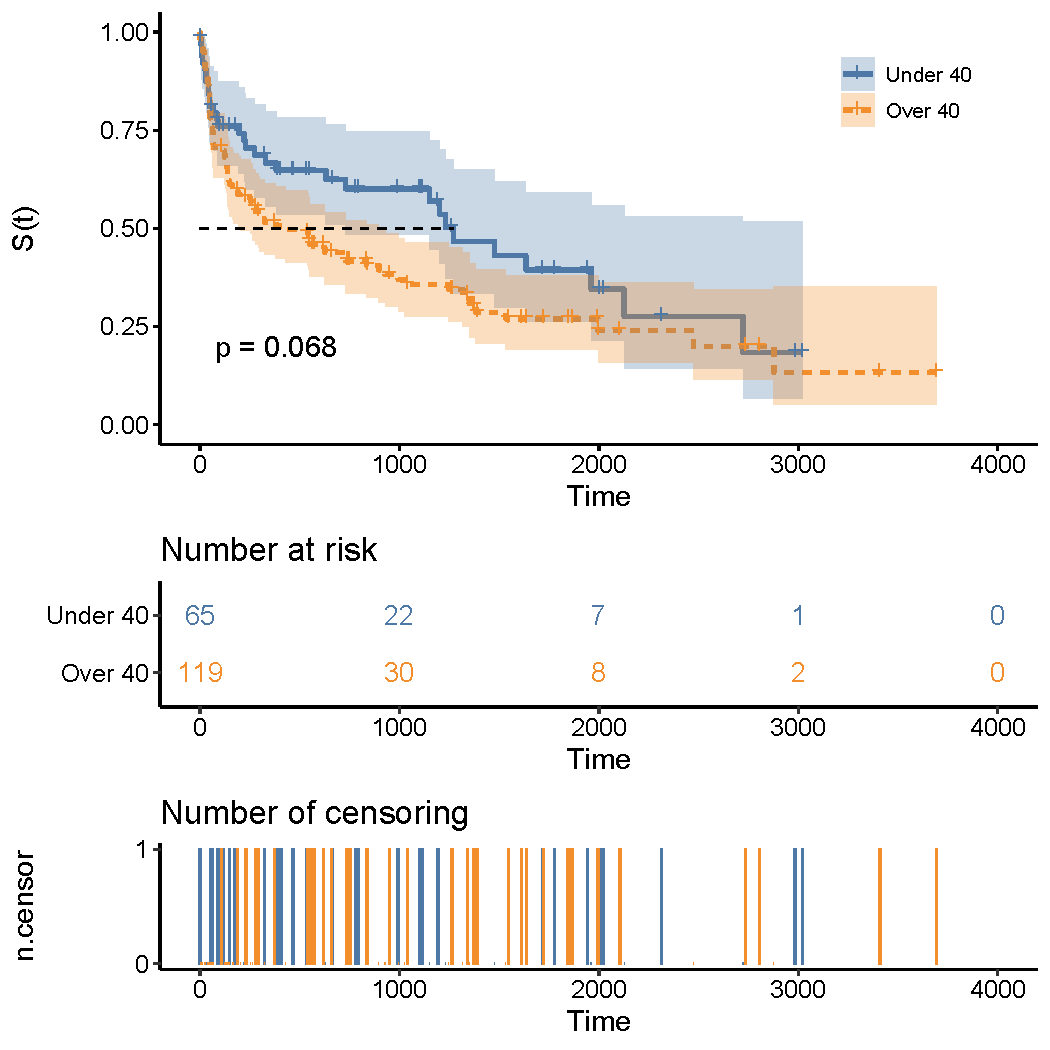
\includegraphics[width=\textwidth]{figures/survival/stanford_km_annotated}
  \caption{Annotated}
  \label{fig:stanford_km:annotated}
  \end{subfigure}
\caption{
Kaplan-Meier plot of the Stanford heart transplant dataset. Censored patients are displayed with marks.
The version on the right adds additional annotations, such as
subplots for patients at risk and censoring events,
the \pvalue from \texttt{survdiff}, and a median reference line.
}
\label{fig:stanford_km}
\end{figure}

\subsubsection{Initialization}
\label{additional:Survival:Rcode:init}

\begin{lstlisting}[language=R]
> install.packages(c("survival", "survminer"))
> library("survival")
> library("survminer")

> df <- stanford2
> df$agecat <- cut(df$age, breaks=c(0,40, Inf), labels=c('Under 40', 'Over 40'), right=FALSE)
> df <- df[with(df, order(time)),]

> df[1:5,c('time', 'status', 'age', 'agecat', 't5')]
    time status age   agecat   t5
21   0.5      1  41  Over 40 0.87
133  1.0      1  21 Under 40 0.47
184  1.0      0  27 Under 40   NA
16   1.0      1  54  Over 40 0.47
183  2.0      0  39 Under 40   NA
> summary(df[c('time', 'agecat', 't5')])
      time              agecat          t5
 Min.   :   0.50   Under 40: 65   Min.   :0.000
 1st Qu.:  64.75   Over 40 :119   1st Qu.:0.690
 Median : 351.00                  Median :1.040
 Mean   : 696.94                  Mean   :1.117
 3rd Qu.:1160.75                  3rd Qu.:1.460
 Max.   :3695.00                  Max.   :3.050
                                  NA's   :27
\end{lstlisting}

\subsubsection{Kaplan-Meier Model}
\label{additional:Survival:Rcode:km}

\begin{lstlisting}[language=R]
> km.model <- survfit(Surv(time, status) ~ agecat, data=df, type='kaplan-meier')
> summary(km.model)$table
                records n.max n.start events   *rmean *se(rmean) median 0.95LCL 0.95UCL
agecat=Under 40      65    65      65     32 1520.783   220.1031   1271     731      NA
agecat=Over 40      119   119     119     81 1123.229   143.3516    431     202     897

> survdiff(Surv(time, status) ~ agecat, data=df)
Call:
survdiff(formula = Surv(time, status) ~ agecat, data = df)

                  N Observed Expected (O-E)^2/E (O-E)^2/V
agecat=Under 40  65       32     41.3      2.10      3.32
agecat=Over 40  119       81     71.7      1.21      3.32

 Chisq= 3.3  on 1 degrees of freedom, p= 0.07

> pdf('~/stanford_km.pdf')
> ggsurvplot(km.model, xlab='Time', ylab='S(t)', size = 1, linetype = 'strata', palette=c('#4e79a7', '#f28e2b'), conf.int = TRUE, legend = c(0.85, 0.85), legend.y = 1, legend.title = '', legend.labs = c('Under 40', 'Over 40'))
> dev.off()

> pdf('~/stanford_km_annotated.pdf')
> ggsurvplot(km.model, xlab='Time', ylab='S(t)', size = 1, linetype = 'strata', palette=c('#4e79a7', '#f28e2b'), conf.int = TRUE, legend = c(0.85, 0.85), legend.y = 1, legend.title = '', legend.labs = c('Under 40', 'Over 40'),
pval = TRUE, # Add survdiff p-value
risk.table = TRUE, # Absolute number at risk
risk.table.y.text.col = FALSE, risk.table.col = "strata",
ncensor.plot = TRUE, # plot censored patients vs time
surv.median.line = "h", # add horizontal median
)
> dev.off()
\end{lstlisting}

\subsubsection{Cox Proportional-Hazards Model}
\label{additional:Survival:Rcode:cox}

\begin{lstlisting}[language=R]
> cox.model_age <- coxph(Surv(time, status) ~ age, data=df[!is.na(df$t5), ])
> summary(cox.model_age)
Call:
coxph(formula = Surv(time, status) ~ age, data = df[!is.na(df$t5),
    ])

  n= 157, number of events= 102

       coef exp(coef) se(coef)     z Pr(>|z|)
age 0.02990   1.03035  0.01136 2.633  0.00846 **
---
Signif. codes:  0 ‘***’ 0.001 ‘**’ 0.01 ‘*’ 0.05 ‘.’ 0.1 ‘ ’ 1

    exp(coef) exp(-coef) lower .95 upper .95
age      1.03     0.9705     1.008     1.054

Concordance= 0.595  (se = 0.034 )
Likelihood ratio test= 7.62  on 1 df,   p=0.006
Wald test            = 6.93  on 1 df,   p=0.008
Score (logrank) test = 7.01  on 1 df,   p=0.008

> cox.model_age_t5 <- coxph(Surv(time, status) ~ age + t5, data=df[!is.na(df$t5), ])
> summary(cox.model_age_t5)
Call:
coxph(formula = Surv(time, status) ~ age + t5, data = df[!is.na(df$t5),
    ])

  n= 157, number of events= 102

       coef exp(coef) se(coef)     z Pr(>|z|)
age 0.02961   1.03006  0.01136 2.608  0.00911 **
t5  0.17041   1.18579  0.18326 0.930  0.35243
---
Signif. codes:  0 ‘***’ 0.001 ‘**’ 0.01 ‘*’ 0.05 ‘.’ 0.1 ‘ ’ 1

    exp(coef) exp(-coef) lower .95 upper .95
age     1.030     0.9708     1.007     1.053
t5      1.186     0.8433     0.828     1.698

Concordance= 0.59  (se = 0.034 )
Likelihood ratio test= 8.47  on 2 df,   p=0.01
Wald test            = 7.81  on 2 df,   p=0.02
Score (logrank) test = 7.87  on 2 df,   p=0.02

> anova(cox.model_age, cox.model_age_t5, test='LRT')
Analysis of Deviance Table
 Cox model: response is  Surv(time, status)
 Model 1: ~ age
 Model 2: ~ age + t5
   loglik Chisq Df P(>|Chi|)
1 -447.29
2 -446.86 0.851  1    0.3563
\end{lstlisting}

\subsubsection{Checking Assumptions}
\label{additional:Survival:Rcode:assumptions}

\begin{lstlisting}[language=R]
# proportional hazards
> cox.model_age.ph <- cox.zph(cox.model_age)
> cox.model_age.ph
       chisq df    p
age     0.76  1 0.38
GLOBAL  0.76  1 0.38

> cox.model_age_t5.ph <- cox.zph(cox.model_age_t5)
> cox.model_age_t5.ph
       chisq df    p
age     0.83  1 0.36
t5      2.06  1 0.15
GLOBAL  2.77  2 0.25

> pdf('~/stanford_cox_age_schoenfeld_residuals.pdf')
> ggcoxzph(cox.model_age.ph)
> dev.off()

> pdf('~/stanford_cloglog.pdf')
> plot(km.model, fun='cloglog', xlab='log(t)', ylab='log(-log(S(t)))', col=c('#4e79a7', '#f28e2b'))
> legend('bottomright', inset=.02, legend=c('Under 40', 'Over 40'), col=c('#4e79a7', '#f28e2b'), lty=1:2, box.lty=0)
> dev.off()

# linearity

> pdf('~/stanford_cox_age_martingale_residuals.pdf')
> ggcoxfunctional(Surv(time, status) ~ age + log(age) + sqrt(age), data = df)
> dev.off()

# outliers

> pdf('~/stanford_cox_age_dfbeta.pdf')
> ggcoxdiagnostics(cox.model_age, type = "dfbeta", linear.predictions = FALSE)
> dev.off()

> pdf('~/stanford_cox_age_deviance_residuals.pdf')
> ggcoxdiagnostics(cox.model_age, type = "deviance", linear.predictions = FALSE)
> dev.off()
\end{lstlisting}

\begin{figure}[H]
\centering
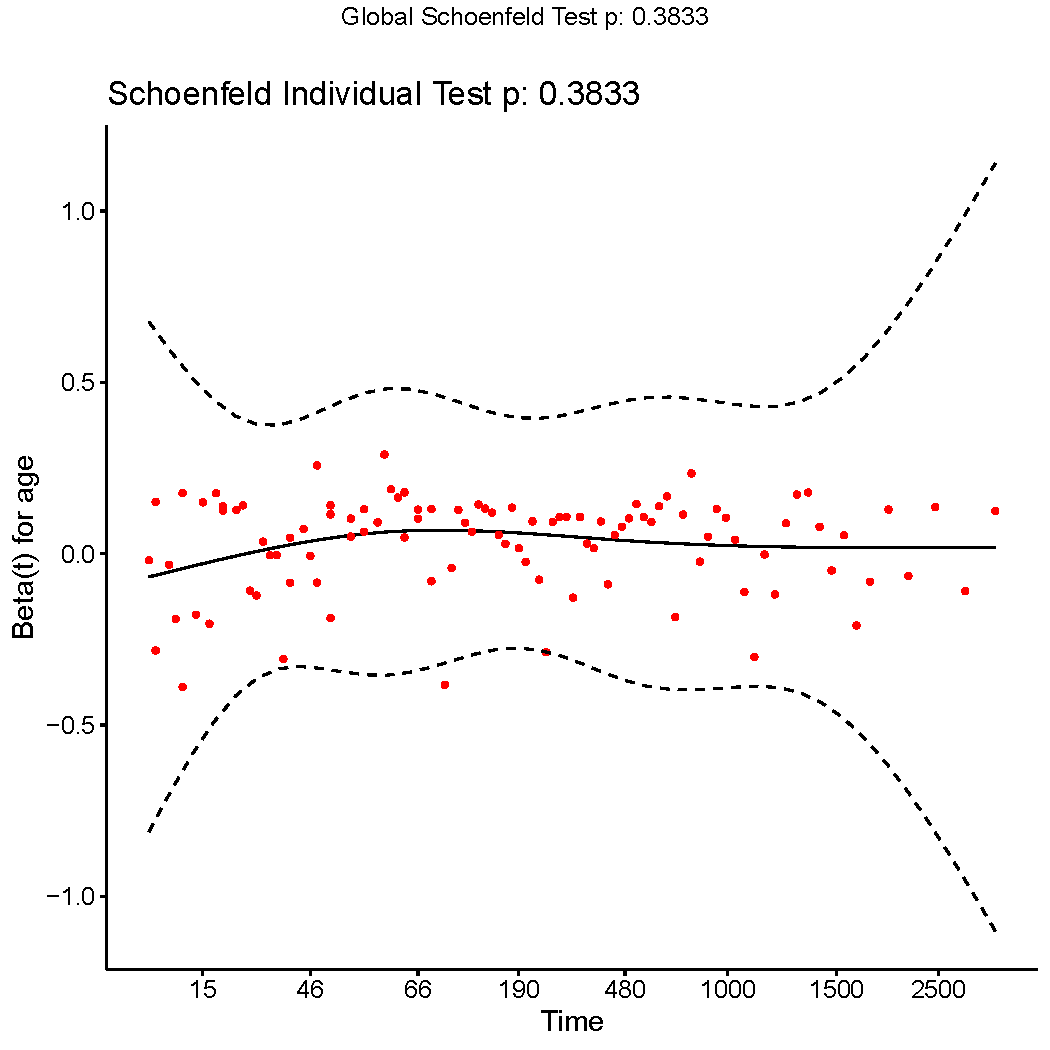
\includegraphics[width=0.7\textwidth]{figures/survival/stanford_cox_age_schoenfeld_residuals}
\vspace{0.2cm}
\caption{
Schoenfeld residual plot for
an univariate Cox model fit to the Stanford heart transplant dataset.
The residuals do not appear dependent on time,
which is supported by the non-significant \pvalue,
and shows that proportional hazards assumption
has been satisfied for this model.
}
\label{fig:cox:schoenfeld_residuals}
\end{figure}

\begin{figure}[H]
\centering
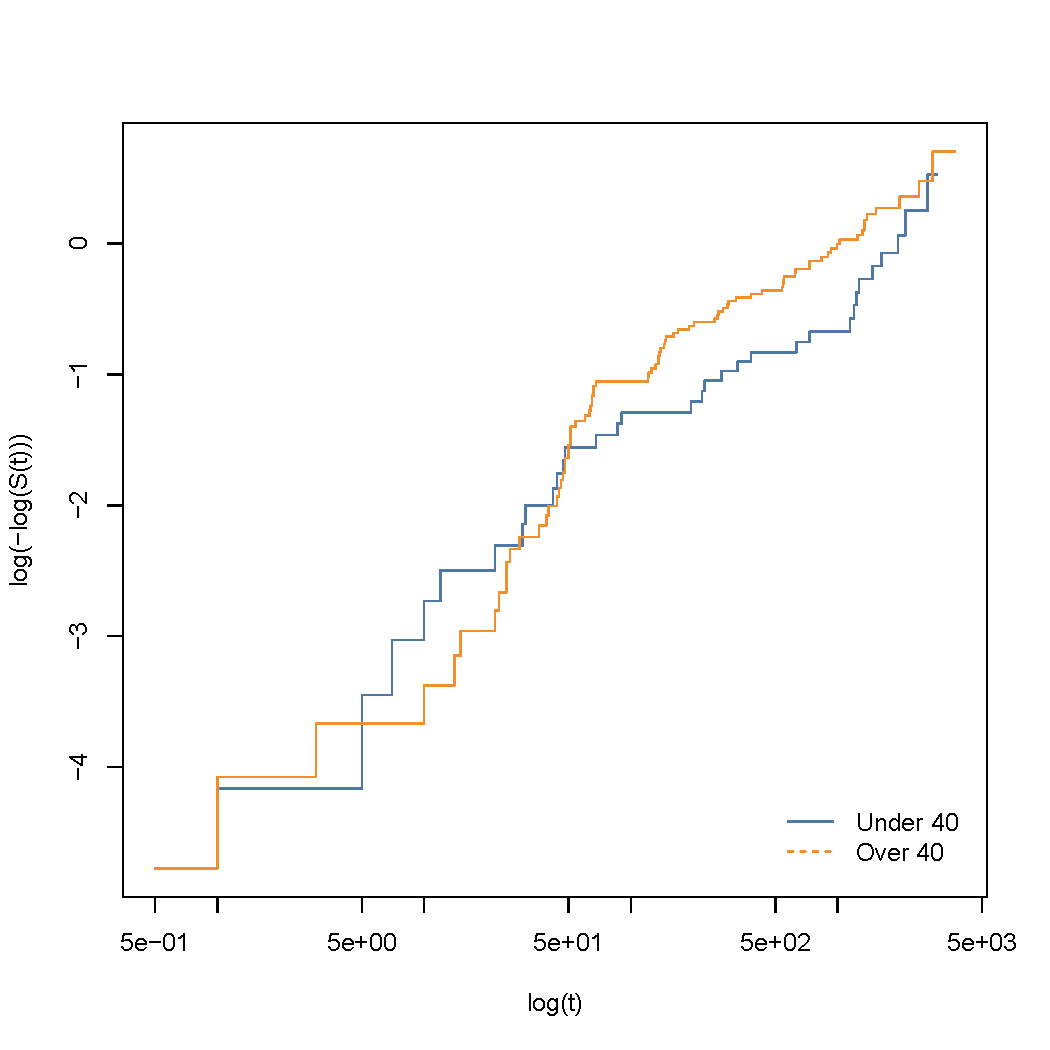
\includegraphics[width=0.7\textwidth]{figures/survival/stanford_cloglog}
\vspace{0.2cm}
\caption{
Complementary log-log plot for categorized patient age
in the Stanford heart transplant dataset.
These curves are not parallel,
the proportional hazards assumption is violated in this variable.
}
\label{fig:stanford_cloglog}
\end{figure}

\begin{figure}[H]
\centering
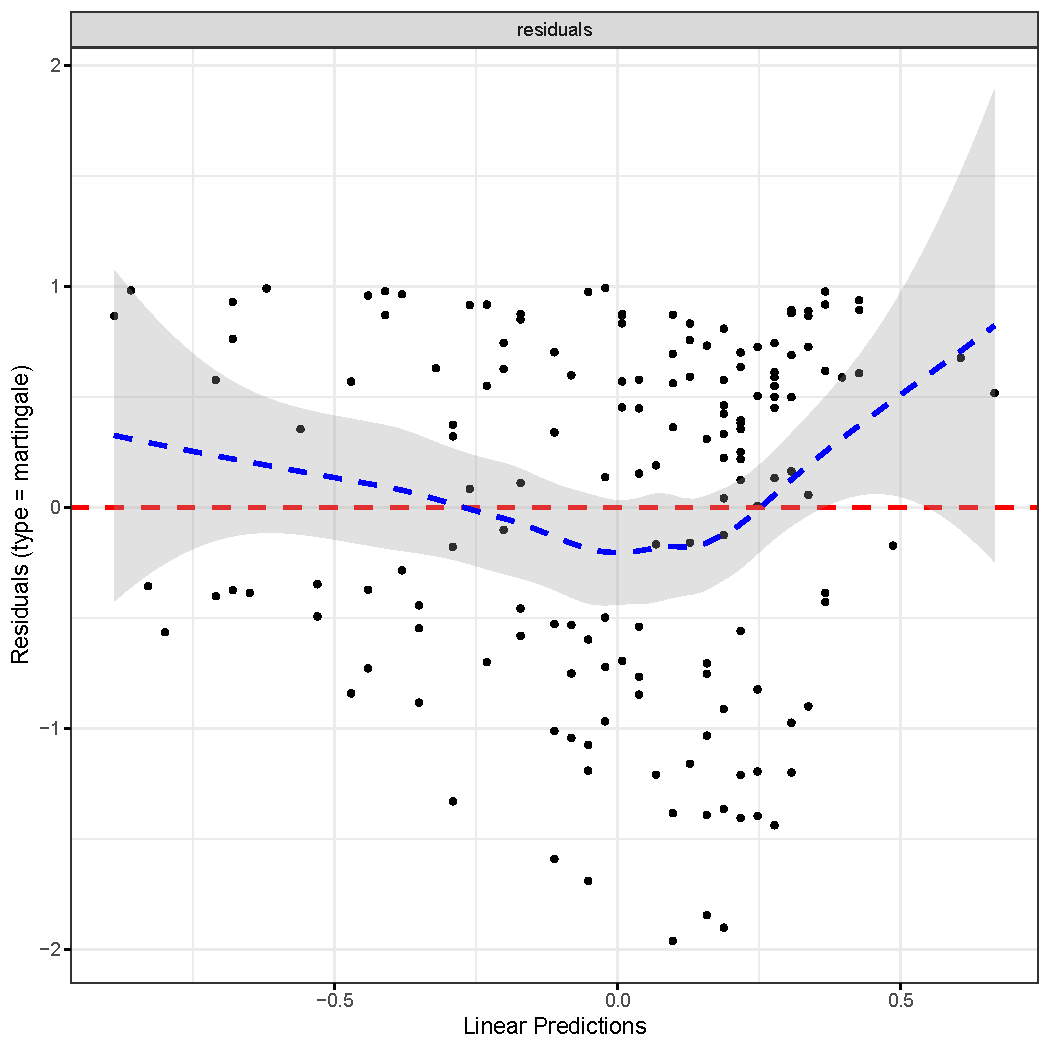
\includegraphics[width=0.7\textwidth]{figures/survival/stanford_cox_age_martingale_residuals}
\vspace{0.2cm}
\caption{
TODO Martingale residuals
}
\label{fig:cox:martingale_residuals}
\end{figure}

\begin{figure}[H]
\centering
  \begin{subfigure}[c]{0.48\textwidth}\centering
  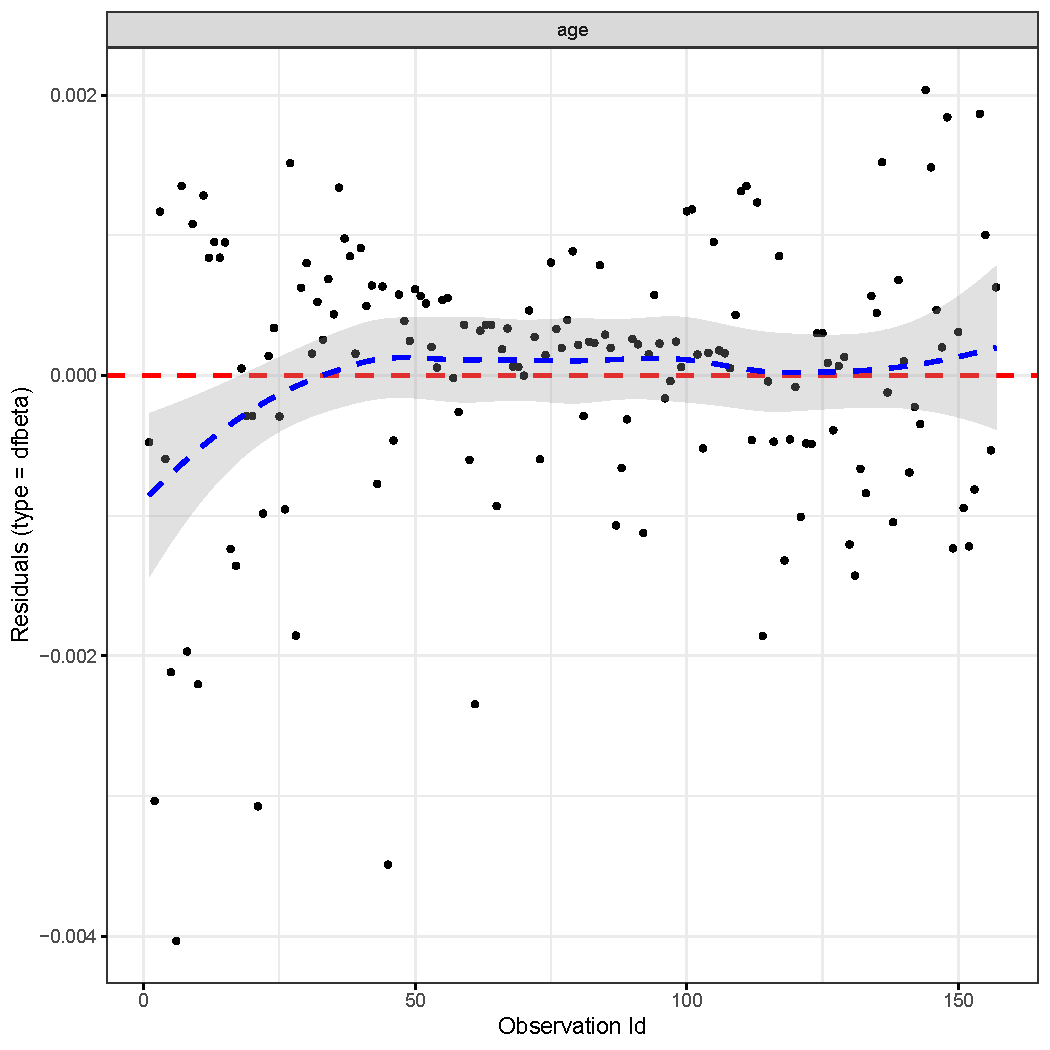
\includegraphics[width=\textwidth]{figures/survival/stanford_cox_age_dfbeta}
  \caption{dfbeta}
  \label{fig:cox:outliers:dfbeta}
  \end{subfigure}
  ~
  \begin{subfigure}[c]{0.48\textwidth}\centering
  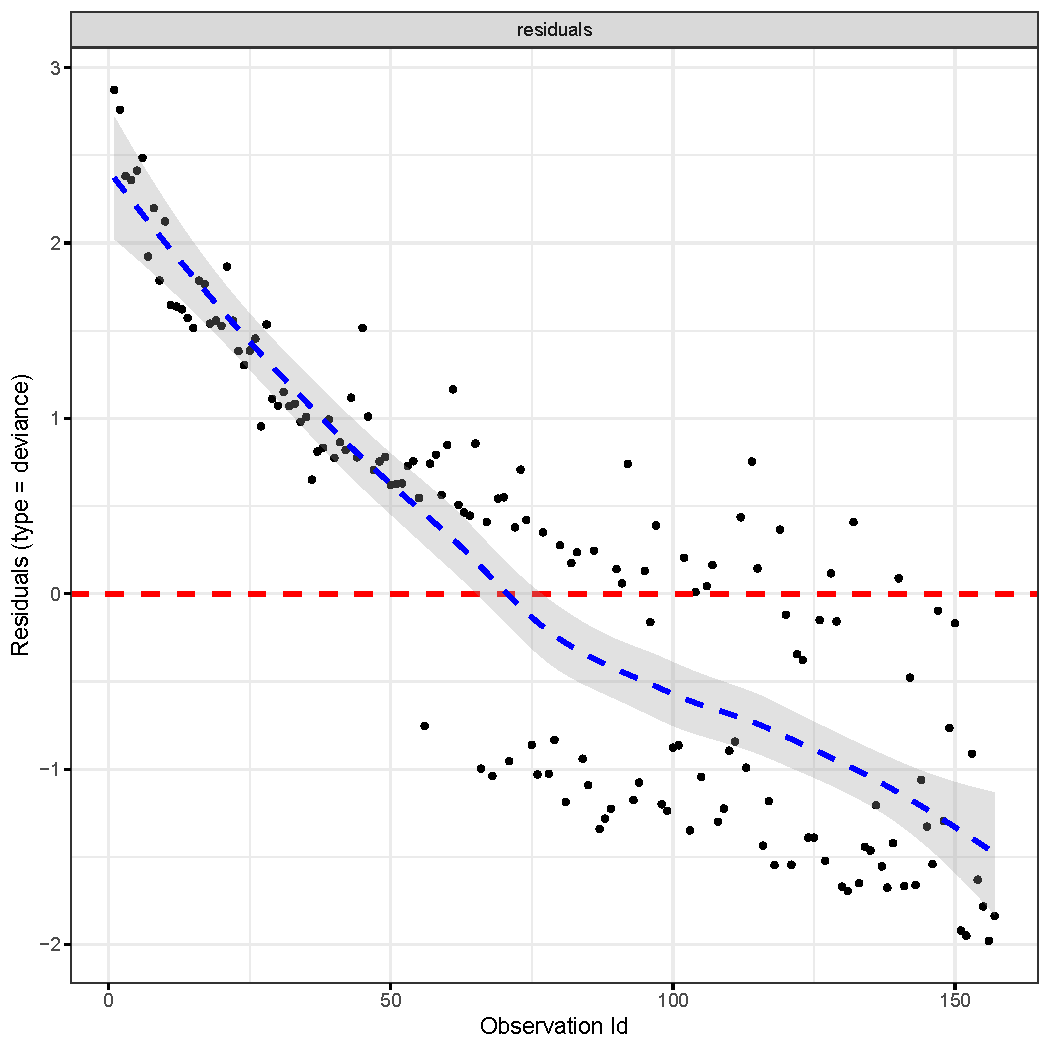
\includegraphics[width=\textwidth]{figures/survival/stanford_cox_age_deviance_residuals}
  \caption{Deviance}
  \label{fig:cox:outliers:deviance}
  \end{subfigure}
\caption{
TODO Outliers
TODO dfbeta and deviance residual plots for
an univariate Cox model fit to the Stanford heart transplant dataset.
}
\label{fig:cox:outliers}
\end{figure}
}
\chapter{Miscellaneous}
\label{chap:misc}

%%%%%%%%%%%%%%%%%%%%%%%%%%%%%%%%%%%%%%%%%%%%%%%%%%%%%%%%
\section{Feature Importance}
\label{misc:feature_importance}
% TODO

%%%%%%%%%%%%%%%%%%%%%%%%%%%%%%%%%%%%%%%%%%%%%%%%%%%%%%%%
\section{Experimental Design \& Hypothesis Testing}
\label{misc:exp_design}
% TODO

%%%%%%%%%%%%%%%%%%%%%%%%%%%%%%%%%%%%%%%%%%%%%%%%%%%%%%%%
\section{Dimensionality Reduction}
\label{misc:m_reduction}
% TODO

%%%%%%%%%%%%%%%%%%%%%%%%%%%%%%%%%%%%%%%%%%%%%%%%%%%%%%%%
\section{Factor Analysis}
\label{misc:factor_ana}
% TODO

}

%==============================================================================

%-----------------------------------------------------------------------------%
% APPENDICES -- OPTIONAL. These are just chapters enumerated by Appendix A, Appendix B, Appendix C...
%-----------------------------------------------------------------------------%
% Start each appendix tex file with '\chapter{Title}'
\appendix
%%%%%%%%%%%%%%%%%%%%%%%%%%%%%%%%%%%%%%%%%%%%%%%%%%%%%%%%
%%%%%%%%%%%%%%%%%%%%%%%%%%%%%%%%%%%%%%%%%%%%%%%%%%%%%%%%
%%%%%%%%%%%%%%%%%%%%%%%%%%%%%%%%%%%%%%%%%%%%%%%%%%%%%%%%
\chapter{\pandas}
\label{pandas}

%%%%%%%%%%%%%%%%%%%%%%%%%%%%%%%%%%%%%%%%%%%%%%%%%%%%%%%%
%%%%%%%%%%%%%%%%%%%%%%%%%%%%%%%%%%%%%%%%%%%%%%%%%%%%%%%%
\section{Basic Commands}
\label{pandas:basic}

\begin{lstlisting}[language=Python]
# IO
df = pd.read_csv('file.csv', header=None)
df['col'] = df['col'].astype(int)
df.to_csv('out.csv')

# descriptive commands
df.describe(); df.columns; df.shape;

# aggregation commands
df.sum(); df.cumsum();
df.min(); df.max(); df.idxmin(); df.idxmax();
df.mean(); df.std(); df.median(); df.mode();

# extract all rows from one column
df_y = df.loc[:, ['y']]

# select by value
df_selection = df.loc[( ((df['x'] == x_value) & (df['y'] == y_value)) | (df['z'] > z_value))]

# select by value and assign new value
df.loc[(df['x'] == x_value), 'y'] = y_value

# select with query
df_selection = df.query('x > 0')

# select with isin
df_selection = df.isin({'x': [x_value1, x_value2], 'y': [y_value]})

# select row by index
series = df.iloc[0]

# apply an arbitrary function
def func(x, y):
  return x*np.sin(y)
df['z'] = np.vectorize(func)(df['x'], df['y'])

# iterate through rows (slow!)
for index, row in df.iterrows():
  x_value = row['x']

# construct from rows
rows_list = []
for nrow in range(nrows):
  rows_list.append({'x':x_value, 'y':y_value})
df = pd.DataFrame(rows_list)
df = df[['x', 'y']]

# rename columns
df = df.rename({'old': 'new'}, axis='columns')

# sort
df = df.sort_values(by=['x', 'y'], ascending=[True, False]).reset_index(drop=True)

# group by, while dropping new count column and duplicates
df = df.groupby(['x', 'y', 'z']).size().to_frame(name = 'count').reset_index().drop(['count'], axis=1).drop_duplicates()

# return duplicate rows
columns_to_check_for_duplicates = ['x', 'y']
df_duplicates = df[df.duplicated(subset=columns_to_check_for_duplicates, keep=False)]

# shuffling
df = df.sample(frac=1., replace=False, random_state=rnd_seed).reset_index(drop=True)

# drop columns
df = df.drop(['col_to_drop1', 'col_to_drop2'], axis=1)

# fill nans, for all columns and per column
df = df.fillna(0.0)
df = df.fillna(value={'x': x_nan_value, 'z': y_nan_value})
\end{lstlisting}

\clearpage

%%%%%%%%%%%%%%%%%%%%%%%%%%%%%%%%%%%%%%%%%%%%%%%%%%%%%%%%
%%%%%%%%%%%%%%%%%%%%%%%%%%%%%%%%%%%%%%%%%%%%%%%%%%%%%%%%
\section{Joining}
\label{pandas:join}

\noindent See the \href{https://pandas.pydata.org/pandas-docs/stable/user_guide/merging.html}{documentation} and this \href{http://chrisalbon.com/python/data_wrangling/pandas_join_merge_dataframe/}{useful guide}.

\begin{lstlisting}[language=Python]
df = pd.merge(df_l, df_r, left_on='id_left', right_on='id_right', how='left')
\end{lstlisting}

%%%%%%%%%%%%%%%%%%%%%%%%%%%%%%%%%%%%%%%%%%%%%%%%%%%%%%%%
%%%%%%%%%%%%%%%%%%%%%%%%%%%%%%%%%%%%%%%%%%%%%%%%%%%%%%%%
\section{Pivoting}
\label{pandas:pivoting}

\subsubsection{pivot}
\label{pandas:pivoting:pivot}

\noindent \href{http://pandas.pydata.org/pandas-docs/stable/reference/api/pandas.DataFrame.pivot.html}{\texttt{pivot} documentation}.

\begin{lstlisting}[language=Python]
DataFrame.pivot(index=None, columns=None, values=None)
\end{lstlisting}

\begin{figure}[H]
\centering
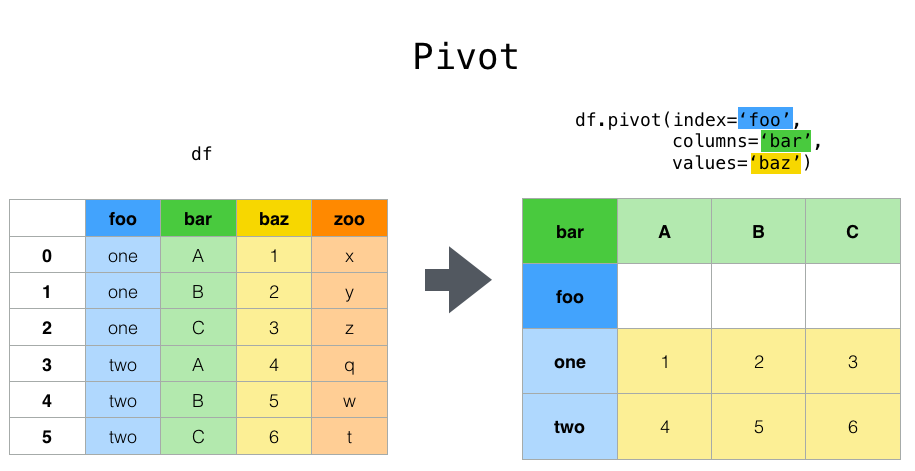
\includegraphics[width=0.85\textwidth]{figures/pandas/reshaping_pivot.png}
\caption{
Example \pandas \texttt{pivot} operation, from the package \href{http://pandas.pydata.org/pandas-docs/stable/user_guide/reshaping.html}{documentation}.
}
\label{fig:pandas:pivot}
\end{figure}

\subsubsection{pivot\_table}
\label{pandas:pivoting:pivot_table}

\noindent \href{https://pandas.pydata.org/pandas-docs/stable/reference/api/pandas.pivot_table.html}{\texttt{pivot\_table} documentation}.

\begin{lstlisting}[language=Python]
pandas.pivot_table(data, values=None, index=None, columns=None, aggfunc='mean', fill_value=None, margins=False, dropna=True, margins_name='All')
\end{lstlisting}

\begin{figure}[H]
\centering
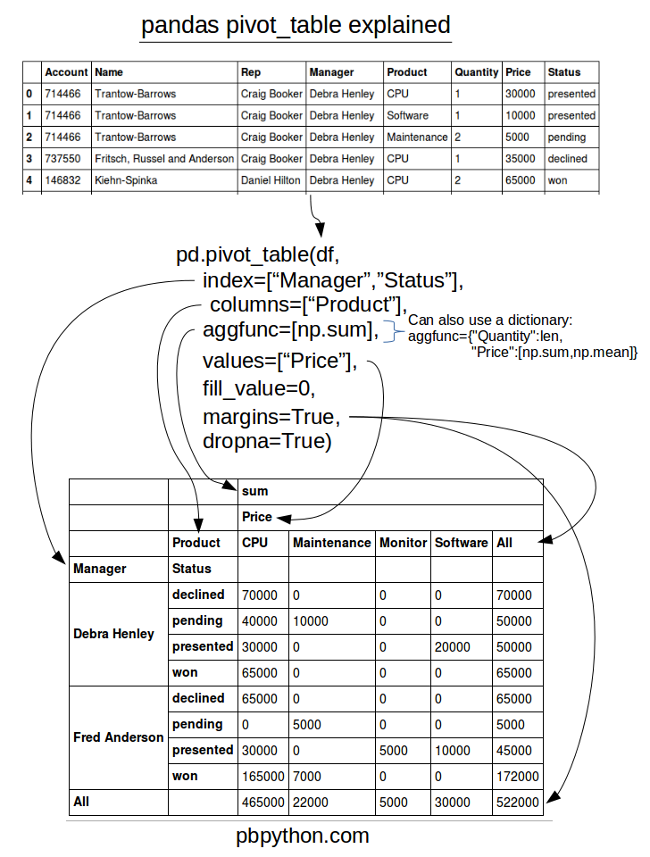
\includegraphics[width=0.95\textwidth]{figures/pandas/pivot-table-datasheet.png}
\caption{
Example \pandas \texttt{pivot\_table} operation, by \href{http://pbpython.com/pandas-pivot-table-explained.html}{Chris Moffitt}.
}
\label{fig:pandas:pivot_table}
\end{figure}
}
%%%%%%%%%%%%%%%%%%%%%%%%%%%%%%%%%%%%%%%%%%%%%%%%%%%%%%%%
%%%%%%%%%%%%%%%%%%%%%%%%%%%%%%%%%%%%%%%%%%%%%%%%%%%%%%%%
\chapter{\sql}
\label{sql}

%%%%%%%%%%%%%%%%%%%%%%%%%%%%%%%%%%%%%%%%%%%%%%%%%%%%%%%%
%%%%%%%%%%%%%%%%%%%%%%%%%%%%%%%%%%%%%%%%%%%%%%%%%%%%%%%%
\section{Basic Commands}
\label{sql:basic}
% TODO

}
%%%%%%%%%%%%%%%%%%%%%%%%%%%%%%%%%%%%%%%%%%%%%%%%%%%%%%%%
%%%%%%%%%%%%%%%%%%%%%%%%%%%%%%%%%%%%%%%%%%%%%%%%%%%%%%%%
%%%%%%%%%%%%%%%%%%%%%%%%%%%%%%%%%%%%%%%%%%%%%%%%%%%%%%%%
\chapter{\pyspark}
\label{pyspark}

%%%%%%%%%%%%%%%%%%%%%%%%%%%%%%%%%%%%%%%%%%%%%%%%%%%%%%%%
%%%%%%%%%%%%%%%%%%%%%%%%%%%%%%%%%%%%%%%%%%%%%%%%%%%%%%%%
\section{Basic Commands}
\label{pyspark:basic}

\begin{lstlisting}[language=Python]
import pyspark.sql.functions as F
from pyspark.sql.window import Window
from pyspark.sql.types import IntegerType, DoubleType

# IO
df = spark.read.parquet('s3a://bucket/table')
df = df.withColumn('col', F.col('col').cast(IntegerType()))
df.write.save('s3a://bucket/table.parquet')

# descriptive commands
df.describe().show(); df.printSchema();
df.show(10); df.limit(10).toPandas();

# select columns
df_y = df.select('x', 'y')

# get distinct values
df_y_distinct = df.select('y').distinct()

# select by value
df_selection = df.where( ((F.col('x') == x_value) & (F.col('y') == y_value)) | (F.col('z') < z_value) )
df_selection = df.where( F.col('x').isNotNull() )

# select by value and assign new value
df = df.withColumn('y', F.when( F.col('x') == x_value, F.lit(y_value) ).otherwise(F.col('y')))

# select where isin, and not (~) isin, some_list
df_selection = df.where(F.col('x').isin(some_list))
df_selection = df.where(~F.col('x').isin(some_list))

# apply an arbitrary function - slow unless written in scala!
def func(x, y):
	return x*np.sin(y)
func_udf = F.udf(func, DoubleType())
df = df.withColumn('z', func_udf('x', 'y'))

# rename columns
df = df.withColumnRenamed('old', 'new')

# order by
df = df.orderBy(['x', 'y'], ascending=[True, False])

# group by, while counting rows and aggregating max date
df = df.groupBy('x', 'y', 'z').agg(F.count('*').alias('count'), F.max('date_col').alias('max_date'))

# group by, get mode of state per patient - deterministically (alphabetical order)
# can be expanded to additional columns, each with their own .join(df.groupBy()...) statements
df.select('patient').distinct().join(
df.where(F.col('state').isNotNull())
	.groupBy(['patient', 'state']).count().alias('c')
	.withColumn('row_num', F.row_number().over(Window().partitionBy('patient').orderBy(F.col('c').desc(), F.col('state'))))
	.where(F.col('row_num') == 1)
	.select('patient', 'state')
, 'patient', 'left')

# return duplicate rows
df.join(df, df.groupBy('x', 'y').agg(F.count('*').alias('c')).where(1 < F.('c')), ['x', 'y'], 'left_semi')

# drop columns
df = df.drop('col_to_drop1', 'col_to_drop2')

cols_to_drop = ['col1', 'col2']
df = df.drop(*cols_to_drop)

# fill nans, for all columns and per column - other syntaxes are also available
df = df.fillna(0.0)
df = df.fillna({'x': x_nan_value, 'z': y_nan_value})

# run a SQL query, note you must register the needed dataframes as tables first
df.registerTempTable('df')
spark.sql('select * from df limit 10').show(10)
\end{lstlisting}

%%%%%%%%%%%%%%%%%%%%%%%%%%%%%%%%%%%%%%%%%%%%%%%%%%%%%%%%
%%%%%%%%%%%%%%%%%%%%%%%%%%%%%%%%%%%%%%%%%%%%%%%%%%%%%%%%
\section{Joining}
\label{pyspark:join}

\noindent See the
\href{https://spark.apache.org/docs/latest/api/python/reference/api/pyspark.sql.DataFrame.join.html#pyspark-sql-dataframe-join}{documentation}
and this
\href{http://www.learnbymarketing.com/1100/pyspark-joins-by-example/}{useful guide}.
In addition to the standard types of joins \texttt{left\_semi}, or \texttt{leftsemi},
is very useful for filtering the left table to the matching rows in the join condition,
without actually joining any columns from the right table.

\begin{lstlisting}[language=Python]
df = df_l.join(df_r, df_l['id_left'] == df_r['id_right'], 'left')
\end{lstlisting}

%%%%%%%%%%%%%%%%%%%%%%%%%%%%%%%%%%%%%%%%%%%%%%%%%%%%%%%%
%%%%%%%%%%%%%%%%%%%%%%%%%%%%%%%%%%%%%%%%%%%%%%%%%%%%%%%%
\section{Pivoting}
\label{pyspark:pivoting}

\noindent \href{https://spark.apache.org/docs/latest/api/python/reference/api/pyspark.sql.GroupedData.pivot.html#pyspark-sql-groupeddata-pivot}{\texttt{pivot} documentation},
and
\href{https://sparkbyexamples.com/pyspark/pyspark-pivot-and-unpivot-dataframe/}{examples}.

\begin{lstlisting}[language=Python]
df.groupBy('product').pivot('state').sum('cost')
\end{lstlisting}
}
%%%%%%%%%%%%%%%%%%%%%%%%%%%%%%%%%%%%%%%%%%%%%%%%%%%%%%%%
%%%%%%%%%%%%%%%%%%%%%%%%%%%%%%%%%%%%%%%%%%%%%%%%%%%%%%%%
%%%%%%%%%%%%%%%%%%%%%%%%%%%%%%%%%%%%%%%%%%%%%%%%%%%%%%%%
\chapter{Coding Concepts}
\label{coding}

%%%%%%%%%%%%%%%%%%%%%%%%%%%%%%%%%%%%%%%%%%%%%%%%%%%%%%%%
%%%%%%%%%%%%%%%%%%%%%%%%%%%%%%%%%%%%%%%%%%%%%%%%%%%%%%%%
\section{Sorting Algorithms}
\label{coding:sorts}

\begin{table}[H]
\centering
\begingroup
\renewcommand*{\arraystretch}{1}
\begin{tabular}{c c c c c c}
\hline
Name & Best & Average & Worst & Memory & Links \\
\hline
\hline
\multirow{2}{*}{Quicksort} & \multirow{2}{*}{$\order{n \log{n}}$} & \multirow{2}{*}{$\order{n \log{n}}$} & \multirow{2}{*}{$\order{n^{2}}$} & $\order{\log{n}}$, avg & \multirow{2}{*}{\href{https://youtu.be/XE4VP_8Y0BU}{Computerphile}, \href{https://youtu.be/SLauY6PpjW4}{HR}} \\
 & & & & $\order{n}$, worst & \\
Merge Sort & $\order{n \log{n}}$ & $\order{n \log{n}}$ & $\order{n \log{n}}$ & $\order{n}$ & \href{https://youtu.be/kgBjXUE_Nwc}{Computerphile}, \href{https://youtu.be/KF2j-9iSf4Q}{HR} \\
Bubble Sort & $\order{n}$ & $\order{n^{2}}$ & $\order{n^{2}}$ & $\order{1}$ & \href{https://youtu.be/kgBjXUE_Nwc}{Computerphile}, \href{https://youtu.be/6Gv8vg0kcHc}{HR} \\
Insertion Sort & $\order{n}$ & $\order{n^{2}}$ & $\order{n^{2}}$ & $\order{1}$ & \href{https://youtu.be/pcJHkWwjNl4}{Computerphile} \\
Heapsort & $\order{n \log{n}}$ & $\order{n \log{n}}$ & $\order{n}$ & $\order{1}$ & \href{https://youtu.be/2DmK_H7IdTo}{Michael Sambol} \\
Bogosort & $\order{n}$ & $\order{\left(n+1\right)!}$ & $\infty$ & $\order{1}$ & --- \\
\hline
\end{tabular}

% TODO add Heapsort, Shellsort, Tree Sort

\endgroup
\caption{
A collection of sorting algorithms with time complexities.
}
\label{tab:sorting_table}
\end{table}

% TODO add heapsort

%%%%%%%%%%%%%%%%%%%%%%%%%%%%%%%%%%%%%%%%%%%%%%%%%%%%%%%%
%%%%%%%%%%%%%%%%%%%%%%%%%%%%%%%%%%%%%%%%%%%%%%%%%%%%%%%%
\section{Other}
\label{coding:other}

%%%%%%%%%%%%%%%%%%%%%%%%%%%%%%%%%%%%%%%%%%%%%%%%%%%%%%%%
\subsection{Binary Tree Search}
\label{coding:other:binary_tree_search}
% TODO
% TODO should probably be moved under BFS or DFS
% https://youtu.be/P3YID7liBug

%%%%%%%%%%%%%%%%%%%%%%%%%%%%%%%%%%%%%%%%%%%%%%%%%%%%%%%%
\subsection{Breadth First Search (BFS)}
\label{coding:other:bfs}
% TODO

\subsubsection{Dijkstra's Algorithm}
\label{coding:other:bfs:dijkstra}
% TODO
% https://youtu.be/GazC3A4OQTE

%%%%%%%%%%%%%%%%%%%%%%%%%%%%%%%%%%%%%%%%%%%%%%%%%%%%%%%%
\subsection{Depth First Search (DFS)}
\label{coding:other:dfs}
% TODO

%%%%%%%%%%%%%%%%%%%%%%%%%%%%%%%%%%%%%%%%%%%%%%%%%%%%%%%%
\subsection{Linked Lists}
\label{coding:other:lls}
% TODO

}
%%%%%%%%%%%%%%%%%%%%%%%%%%%%%%%%%%%%%%%%%%%%%%%%%%%%%%%%
%%%%%%%%%%%%%%%%%%%%%%%%%%%%%%%%%%%%%%%%%%%%%%%%%%%%%%%%
%%%%%%%%%%%%%%%%%%%%%%%%%%%%%%%%%%%%%%%%%%%%%%%%%%%%%%%%
\chapter{Probability Distributions}
\label{dist}

% Place these distributions first as they are simple and keep the interesting ones together on the next page
\begin{figure}
  \centering
  \savebox{\largestimage}{
    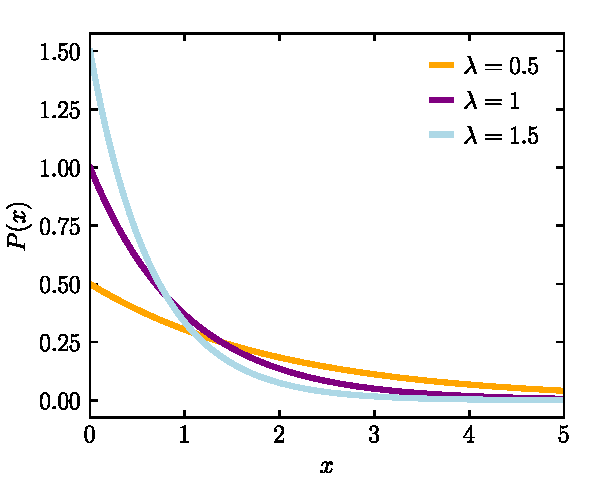
\includegraphics[width=0.47\textwidth]{figures/stats/dist/exp_pdf}
  }% Store largest image in a box

  \begin{subfigure}[b]{0.48\textwidth}\centering
    \raisebox{\dimexpr.5\ht\largestimage-.5\height}{% Adjust vertical height of smaller image
      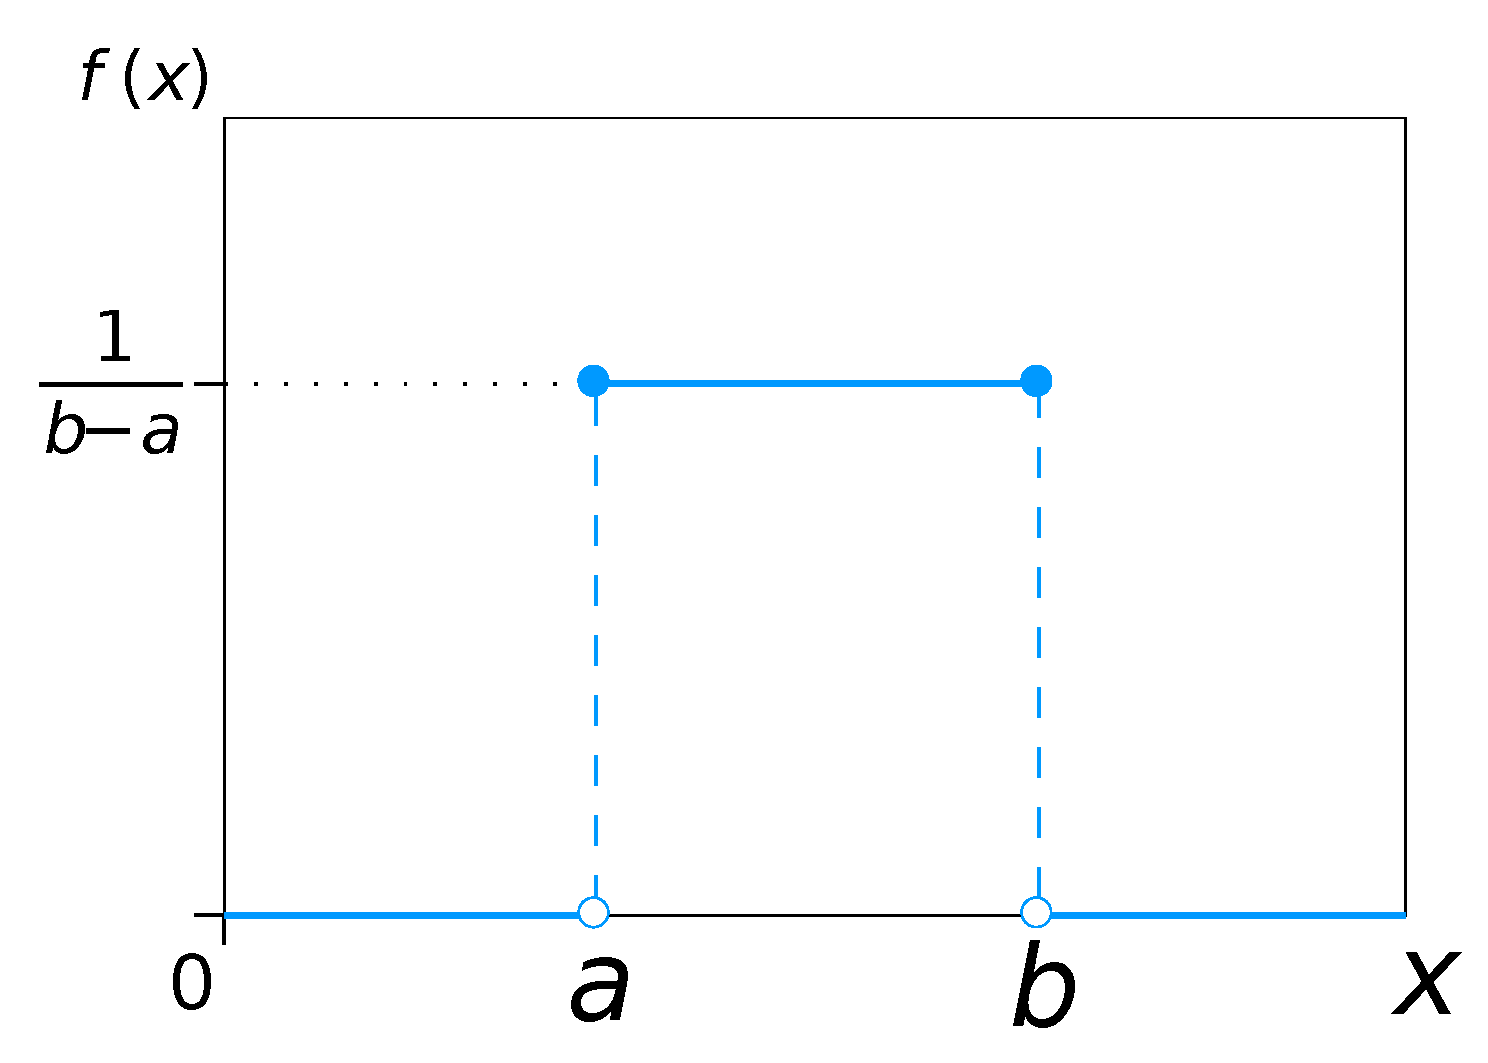
\includegraphics[width=\textwidth]{figures/stats/dist/uniform_pdf}}
  \caption{Uniform Distribution PDF}
  \label{fig:dist:uniform}
  \end{subfigure}
  ~
  \begin{subfigure}[b]{\wd\largestimage}\centering
    \usebox{\largestimage}
  \caption{Exponential Distribution PDF}
  \label{fig:dist:exp}
  \end{subfigure}
\caption{
Uniform and exponential distribution PDFs,
by \href{https://en.wikipedia.org/wiki/File:Uniform_Distribution_PDF_SVG.svg}{AnonMoos}
and \href{https://en.wikipedia.org/wiki/File:Exponential_probability_density.svg}{AkanoToE}.
\label{fig:dist:uniform_exp}
}
\end{figure}

\begin{figure}
  \centering
  \savebox{\largestimage}{
    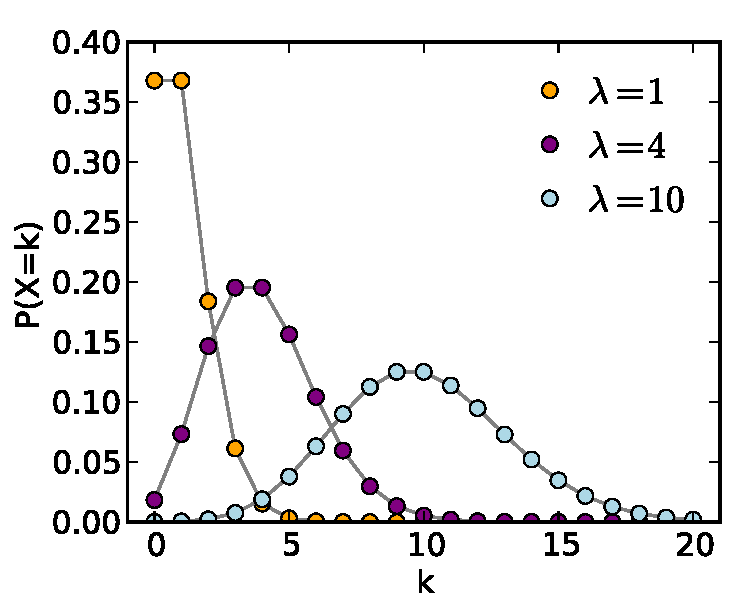
\includegraphics[width=0.47\textwidth]{figures/stats/dist/poisson_pmf}
  }% Store largest image in a box

  \begin{subfigure}[b]{\wd\largestimage}\centering
    \raisebox{\dimexpr.5\ht\largestimage-.5\height}{% Adjust vertical height of smaller image
      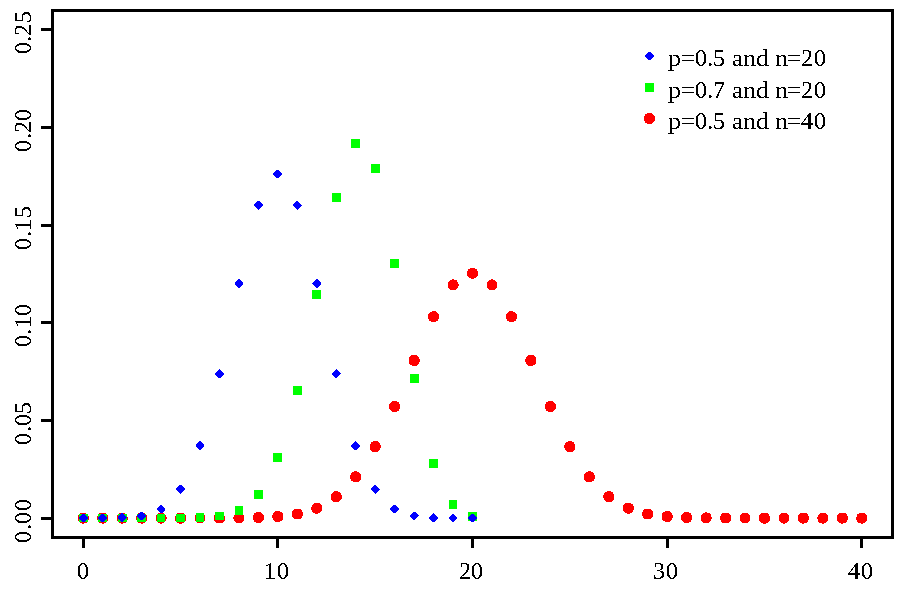
\includegraphics[width=\textwidth]{figures/stats/dist/binomial_pmf}}
  \caption{Binomial Distribution PMF}
  \label{fig:dist:binomial}
  \end{subfigure}
  ~
  \begin{subfigure}[b]{0.48\textwidth}\centering
    \usebox{\largestimage}
  \caption{Poisson Distribution PMF}
  \label{fig:dist:poisson}
  \end{subfigure}
\caption{
Binomial and Poisson distribution PMFs,
by \href{https://en.wikipedia.org/wiki/File:Binomial_distribution_pmf.svg}{Tayste}
and \href{https://en.wikipedia.org/wiki/File:Poisson_pmf.svg}{Skbkekas}.
Both plots have $k$ on the $x$-axis and $P$ on the $y$-axis, and curves for various $n$ and $p$, or $\lambda$.
\label{fig:dist:binomial_poisson}
}
\end{figure}

\begin{figure}
  \centering
  \savebox{\largestimage}{
    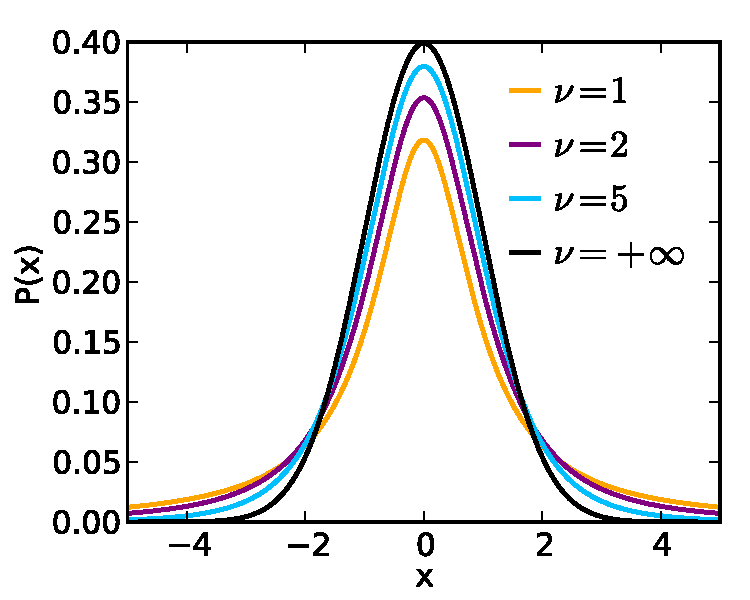
\includegraphics[width=0.47\textwidth]{figures/stats/dist/student_t_pdf}
  }% Store largest image in a box

  \begin{subfigure}[b]{0.48\textwidth}\centering
    \raisebox{\dimexpr.5\ht\largestimage-.5\height}{% Adjust vertical height of smaller image
      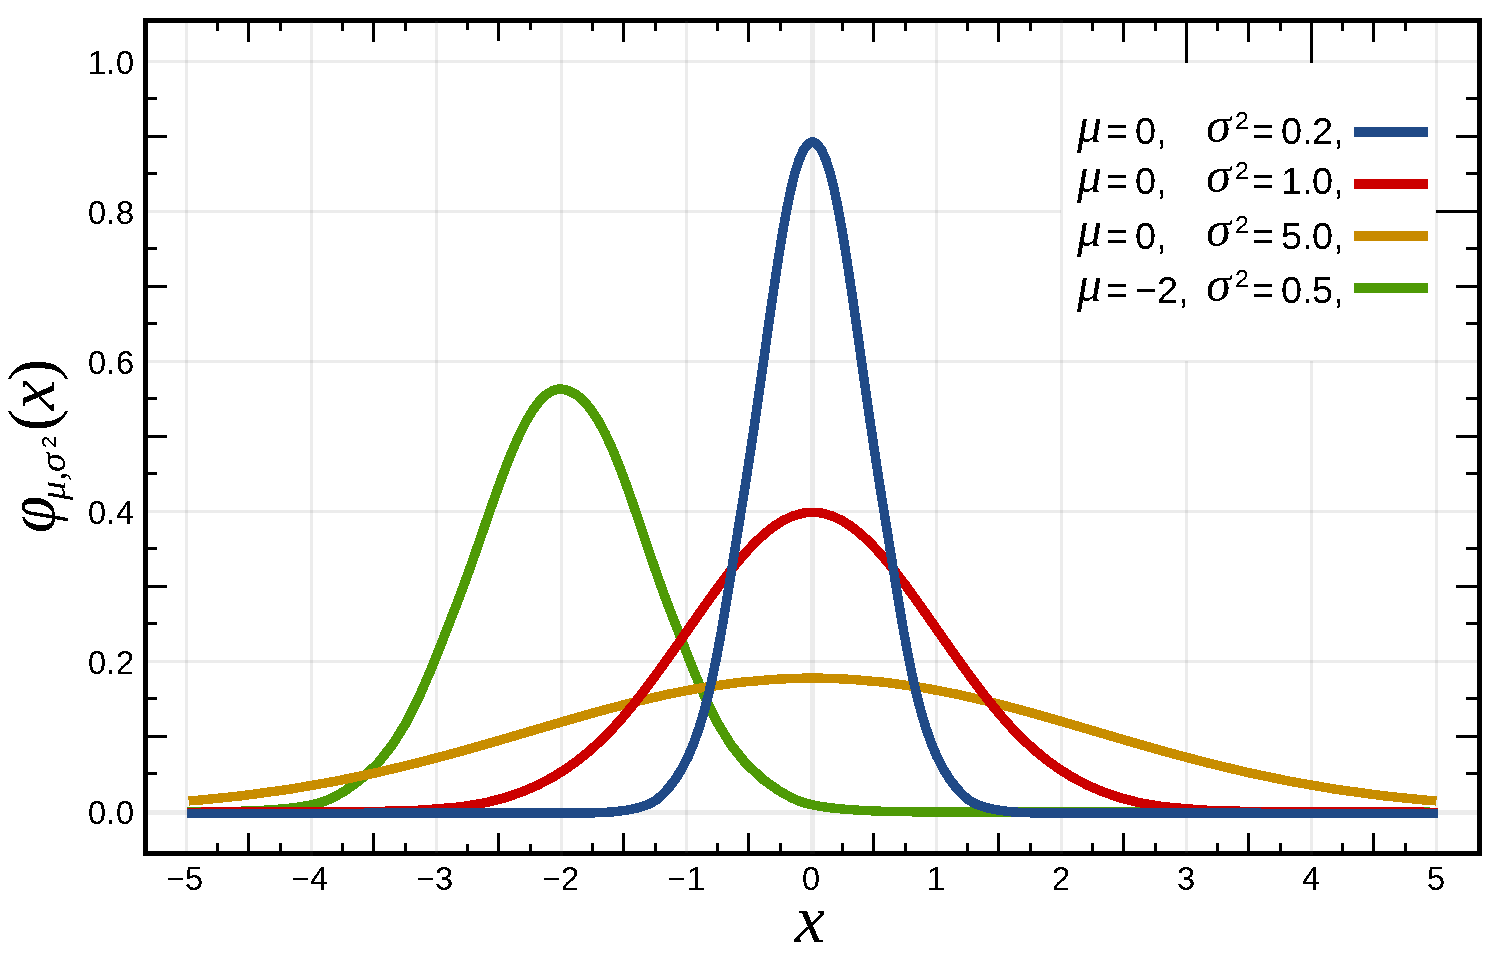
\includegraphics[width=\textwidth]{figures/stats/dist/gaussian_pdf}}
  \caption{Gaussian Distribution PDF}
  \label{fig:dist:gaus}
  \end{subfigure}
  ~
  \begin{subfigure}[b]{\wd\largestimage}\centering
    \usebox{\largestimage}
  \caption{Student's $t$-Distribution PDF}
  \label{fig:dist:student_t}
  \end{subfigure}
\caption{
Gaussian and Student's $t$-distribution PDFs,
by \href{https://en.wikipedia.org/wiki/File:Normal_Distribution_PDF.svg}{Inductiveload}
and \href{https://en.wikipedia.org/wiki/File:Student_t_pdf.svg}{Skbkekas}.
Note that in the limit $\nu \to \infty$ Student's $t$-distribution
approaches the standard normal distribution shown in red.
\label{fig:dist:gaus_student_t}
}
\end{figure}

\begin{figure}
\centering
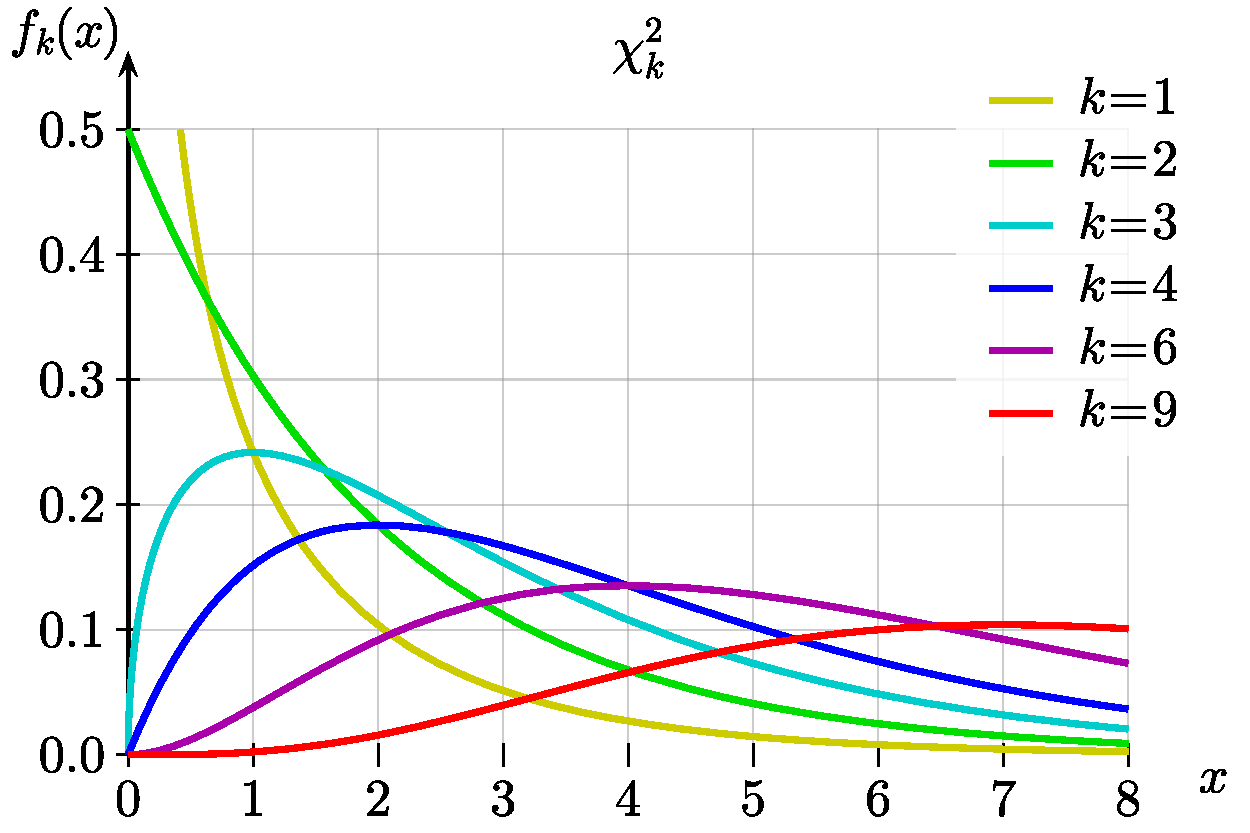
\includegraphics[width=0.7\textwidth]{figures/stats/dist/chi2_pdf}
\caption{
$\chi^{2}$-distribution PDF,
by \href{https://en.wikipedia.org/wiki/File:Chi-square_pdf.svg}{Geek3}.
Here $k$ is being used in lieu of $\nu$ for the number of degrees of freedom.
}
\label{fig:dist:chi2}
\end{figure}

\begin{figure}
\centering
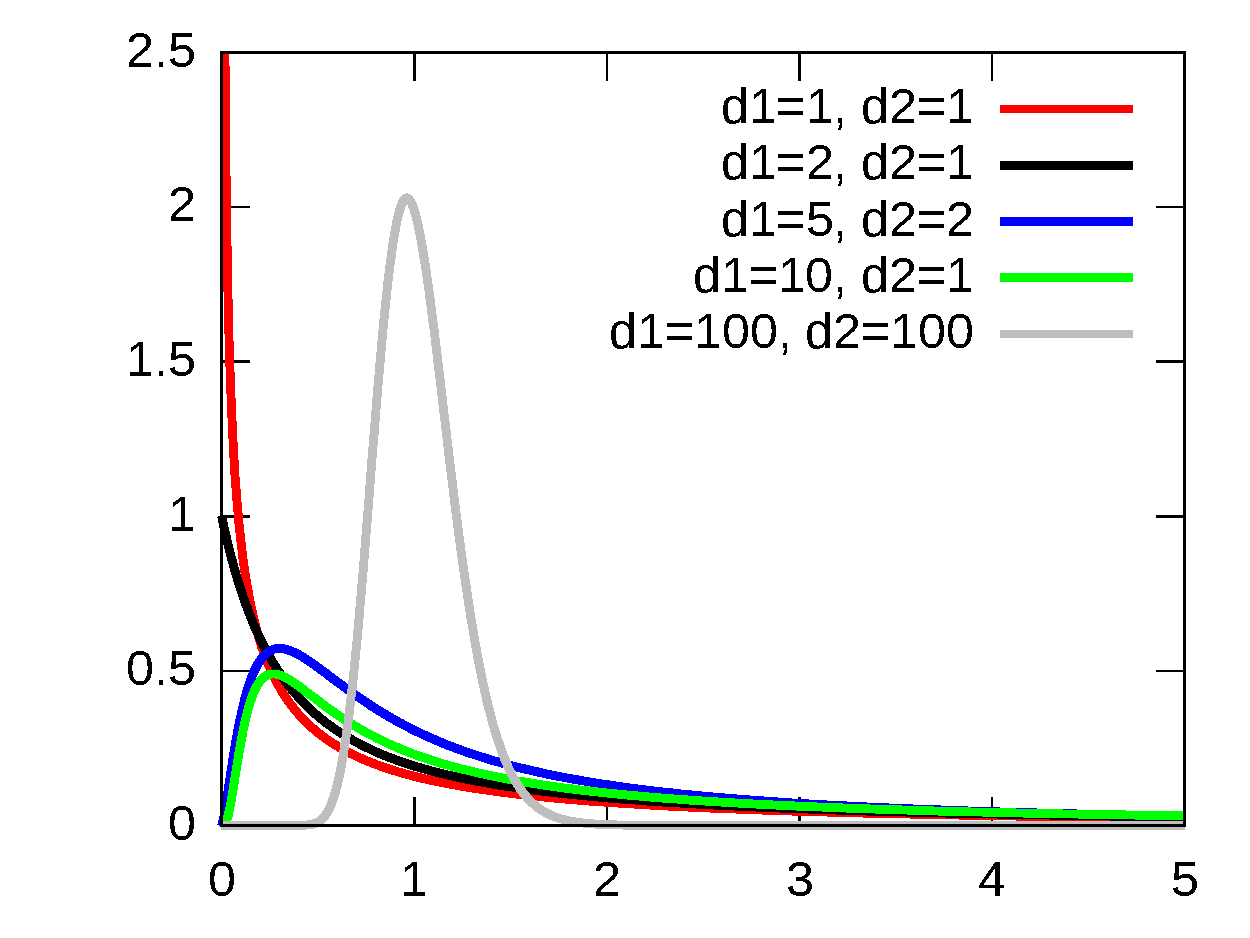
\includegraphics[width=0.7\textwidth,trim={1.5cm 0.1cm 0.1cm 0.1cm},clip]{figures/stats/dist/F_pdf}% trim={<left> <lower> <right> <upper>}
\caption{
$F$-distribution PDF,
by \href{https://en.wikipedia.org/wiki/File:F-distribution_pdf.svg}{IkamusumeFan}.
}
\label{fig:dist:F}
\end{figure}
}
%%%%%%%%%%%%%%%%%%%%%%%%%%%%%%%%%%%%%%%%%%%%%%%%%%%%%%%%%
%%%%%%%%%%%%%%%%%%%%%%%%%%%%%%%%%%%%%%%%%%%%%%%%%%%%%%%%
%%%%%%%%%%%%%%%%%%%%%%%%%%%%%%%%%%%%%%%%%%%%%%%%%%%%%%%%
\chapter{Concepts for Finance}
\label{finance}

%%%%%%%%%%%%%%%%%%%%%%%%%%%%%%%%%%%%%%%%%%%%%%%%%%%%%%%%
%%%%%%%%%%%%%%%%%%%%%%%%%%%%%%%%%%%%%%%%%%%%%%%%%%%%%%%%
\section{Stochastic Processes}
\label{finance:sp}
% TODO

%%%%%%%%%%%%%%%%%%%%%%%%%%%%%%%%%%%%%%%%%%%%%%%%%%%%%%%%
%%%%%%%%%%%%%%%%%%%%%%%%%%%%%%%%%%%%%%%%%%%%%%%%%%%%%%%%
\section{Martingale}
\label{finance:martingale}
% TODO

%%%%%%%%%%%%%%%%%%%%%%%%%%%%%%%%%%%%%%%%%%%%%%%%%%%%%%%%
%%%%%%%%%%%%%%%%%%%%%%%%%%%%%%%%%%%%%%%%%%%%%%%%%%%%%%%%
\section{Wiener Processes}
\label{finance:wiener}
% TODO

%%%%%%%%%%%%%%%%%%%%%%%%%%%%%%%%%%%%%%%%%%%%%%%%%%%%%%%%
%%%%%%%%%%%%%%%%%%%%%%%%%%%%%%%%%%%%%%%%%%%%%%%%%%%%%%%%
\section{Brownian Motion}
\label{finance:brownian}
% TODO

%%%%%%%%%%%%%%%%%%%%%%%%%%%%%%%%%%%%%%%%%%%%%%%%%%%%%%%%
%%%%%%%%%%%%%%%%%%%%%%%%%%%%%%%%%%%%%%%%%%%%%%%%%%%%%%%%
\section{Random Walks}
\label{finance:rand_walk}
% TODO

%%%%%%%%%%%%%%%%%%%%%%%%%%%%%%%%%%%%%%%%%%%%%%%%%%%%%%%%
%%%%%%%%%%%%%%%%%%%%%%%%%%%%%%%%%%%%%%%%%%%%%%%%%%%%%%%%
\section{It\^o's Lemma}
\label{finance:ito_lemma}
% TODO

%%%%%%%%%%%%%%%%%%%%%%%%%%%%%%%%%%%%%%%%%%%%%%%%%%%%%%%%
%%%%%%%%%%%%%%%%%%%%%%%%%%%%%%%%%%%%%%%%%%%%%%%%%%%%%%%%
\section{Black-Scholes Model}
\label{finance:black_scholes}
% TODO

}

%-----------------------------------------------------------------------------%
% BIBLIOGRAPHY -- Change the style to match your discipline's standards.
%-----------------------------------------------------------------------------%
\bibliographystyle{./bib/atlasBibStyleWithTitle}
\cleardoublepage
\normalbaselines %Fixes spacing of bibliography
% \addcontentsline{toc}{chapter}{Bibliography} % not needed on my system
\bibliography{./bib/bib}
%-----------------------------------------------------------------------------%

%-----------------------------------------------------------------------------
\end{document}
